% =============================================================================
% MOCK FINAL EXAM 1 (Simulado 1) -- Macroeconomics I, MPE Insper, 2026/T3
% One source, two PDFs (run each command twice, from Simulados/):
%   Blank exam:
%     pdflatex -jobname=simulado-01-exam simulado-01.tex
%   Solutions + rubric:
%     pdflatex -jobname=simulado-01-solutions "\def\withsolutions{}% =============================================================================
% MOCK FINAL EXAM 1 (Simulado 1) -- Macroeconomics I, MPE Insper, 2026/T3
% One source, two PDFs (run each command twice, from Simulados/):
%   Blank exam:
%     pdflatex -jobname=simulado-01-exam simulado-01.tex
%   Solutions + rubric:
%     pdflatex -jobname=simulado-01-solutions "\def\withsolutions{}% =============================================================================
% MOCK FINAL EXAM 1 (Simulado 1) -- Macroeconomics I, MPE Insper, 2026/T3
% One source, two PDFs (run each command twice, from Simulados/):
%   Blank exam:
%     pdflatex -jobname=simulado-01-exam simulado-01.tex
%   Solutions + rubric:
%     pdflatex -jobname=simulado-01-solutions "\def\withsolutions{}% =============================================================================
% MOCK FINAL EXAM 1 (Simulado 1) -- Macroeconomics I, MPE Insper, 2026/T3
% One source, two PDFs (run each command twice, from Simulados/):
%   Blank exam:
%     pdflatex -jobname=simulado-01-exam simulado-01.tex
%   Solutions + rubric:
%     pdflatex -jobname=simulado-01-solutions "\def\withsolutions{}\input{simulado-01.tex}"
% Check fonts afterwards: pdffonts simulado-01-solutions.pdf  (all Type 1)
% Every number in the key is verified by simulado_codigo/check_simulado_01.py
% =============================================================================
\documentclass[11pt,a4paper]{article}
\usepackage[utf8]{inputenc}
\usepackage[T1]{fontenc}
\usepackage{lmodern}   % Type 1 vector fonts (replaces PK bitmaps)
\usepackage{cmap}      % ToUnicode CMap -> copyable text
\usepackage[english]{babel}
\usepackage{amsmath,amssymb,amsfonts}
\usepackage[a4paper,margin=2.2cm]{geometry}
\usepackage{enumitem}
\usepackage{fancyhdr}
\usepackage{comment}
\def\CommentCutFile{simulado-01.cut} % private cut file: sibling sources build in this folder
\usepackage{xcolor}
\usepackage{booktabs}
\usepackage{microtype}
\usepackage{pgfplots}
\pgfplotsset{compat=1.16}

% ====================== CONFIGURATION ======================
\newif\ifsolucoes
\ifdefined\withsolutions\solucoestrue\else\solucoesfalse\fi

\newcommand{\course}{Macroeconomics I --- MPE Insper}
\newcommand{\examtitle}{Mock Final Exam 1 (Simulado 1)}
\newcommand{\answerheight}{5.2cm}

% ====================== MACHINERY ======================
\ifsolucoes\includecomment{sol}\else\excludecomment{sol}\fi

\pagestyle{fancy}\fancyhf{}
\lhead{\footnotesize\course}
\rhead{\footnotesize\examtitle\ifsolucoes{} --- Solutions and Rubric\fi}
\cfoot{\footnotesize\thepage}
\renewcommand{\headrulewidth}{0.3pt}
\setlength{\headheight}{14pt}

\setlist{topsep=2pt,itemsep=2pt}
\newcounter{questao}

\newcommand{\block}[3]{\bigskip\noindent
  {\large\bfseries\color{blue!55!black}Block #1 --- #2}\par\noindent{\small\textit{(#3)}}\par
  \noindent\rule{\linewidth}{0.3pt}\smallskip}
\newcommand{\question}[1]{\refstepcounter{questao}\medskip\noindent
  \textbf{Question \thequestao.}~#1\par}
\newenvironment{options}{\begin{enumerate}[label=\Alph*.,leftmargin=2.2em,topsep=1pt]}{\end{enumerate}}
\newcommand{\answer}[1]{\ifsolucoes\par\noindent\textbf{Answer:}~#1\fi}
\newcommand{\answerspace}{\ifsolucoes\else\par\textit{Solution:}\vspace{\answerheight}\par\fi}
\newcommand{\step}[2]{\par\smallskip\noindent\textbf{Step --- #1.}~#2}
\newcommand{\intuition}[1]{\par\smallskip\noindent\textit{Intuition.}~#1}
\newcommand{\refbib}[1]{\par\smallskip\noindent{\footnotesize\color{black!60}\textbf{Ref:} #1}}
\newcommand{\gap}[1]{\par\smallskip\noindent{\footnotesize\color{red!55!black}\textbf{Gap targeted:} #1}}
\newcommand{\rubric}[1]{\par\smallskip\noindent\textbf{Rubric.}\begin{itemize}[leftmargin=1.4em,topsep=1pt]#1\end{itemize}}
\newcommand{\res}[1]{\boxed{#1}}

% =============================================================================
\begin{document}
\begin{center}
  {\Large\bfseries \course}\\[2pt]
  {\large \examtitle}\ifsolucoes\\[2pt]\textit{Solutions and Grading Rubric}\fi
\end{center}
\vspace{2pt}

{\footnotesize\noindent\textbf{Instructions.} Four blocks of 25 points each (100 points).
Suggested time: 3 hours. Multiple-choice items: mark the single correct option (no penalty
for wrong answers). \emph{True/False} items: every 2 wrong items cancel 1 right item
(score $=\max\{0,\ \text{right}-\text{wrong}/2\}\times$ item value); blank items do not
count as wrong. Discursive questions: show every step; box your final answers. Numerical
values are illustrative. Notation follows Kurlat (2020).\par}

% =============================================================================
\block{I}{Measurement}{Lecture 1; Kurlat chs.~1--2 \,\textbullet\, 25 points}

\question{(10 points) Objective items.}

\textbf{a)} (3 points) An economy produces two goods. In Year~1, good $X$ costs 10 and
$10$ units are produced; good $Z$ costs 5 and $20$ units are produced. In Year~2, $X$ costs 5
and $20$ units are produced; $Z$ costs 10 and $16$ units are produced. Real GDP growth from
Year~1 to Year~2 measured at Year-1 prices and at Year-2 prices is, respectively:
\begin{options}
\item $40\%$ at Year-1 prices; $4\%$ at Year-2 prices.
\item $4\%$ at Year-1 prices; $40\%$ at Year-2 prices.
\item $30\%$ at Year-1 prices; $30\%$ at Year-2 prices.
\item $40\%$ at Year-1 prices; $30\%$ at Year-2 prices.
\item $20.7\%$ at Year-1 prices; $20.7\%$ at Year-2 prices.
\end{options}
\answer{A}
\begin{sol}
\step{compute}{Nominal: $Y_1=10\cdot10+5\cdot20=200$, $Y_2=5\cdot20+10\cdot16=260$.
Year-2 output at Year-1 prices: $10\cdot20+5\cdot16=280\Rightarrow 280/200-1=\res{40\%}$.
Year-1 output at Year-2 prices: $5\cdot10+10\cdot20=250\Rightarrow 260/250-1=\res{4\%}$.
C is nominal growth ($260/200-1$), E is the Fisher index ($\sqrt{1.40\cdot1.04}-1$), B swaps the bases.}
\refbib{Kurlat \S1.2, pp.~22--25.}
\gap{Lista 1, 1(b)(c): Laspeyres/Paasche arithmetic slips.}
\end{sol}

\medskip
\textbf{b)} (3 points) Why is the GDP of a low-income country, converted into dollars at the
market exchange rate, systematically \emph{lower} than the same GDP converted at purchasing
power parity (PPP)?
\begin{options}
\item Tariffs and transport costs keep traded-goods prices apart across countries, and the market rate cannot close that gap.
\item Non-traded goods and services are cheap where wages are low, and the market rate, set by traded goods, ignores this.
\item The market rate is driven by capital flows rather than by trade, so it undervalues every poor-country currency by the same factor.
\item Large informal sectors are left out of the official statistics, so a big share of production is missing from measured GDP.
\item Quotas and import licences raise traded-goods prices in poor countries, which inflates their measured price level.
\end{options}
\answer{B}
\begin{sol}
\step{mechanism}{The market rate equalises (roughly) the prices of \emph{traded} goods. Non-traded
output (housing, haircuts, public services) is priced off local wages, which are low where
productivity in tradables is low (Balassa--Samuelson). Converting at the market rate values that
output at rich-country prices nobody there pays $\Rightarrow$ understates real output. A and E are
frictions in traded goods (and E goes the wrong way); D lowers GDP at \emph{any} conversion rate, so it
cannot explain the gap between the two; C has no mechanism.}
\refbib{Kurlat \S1.2, pp.~25--27.}
\gap{Lista 1, 1(e): PPP gap explained with trade costs instead of non-tradables.}
\end{sol}

\medskip
\textbf{c)} (2 points, T or F) In a two-good economy, if between two years quantities shift
toward the good whose relative price fell, then real GDP growth measured at initial-year prices
exceeds real GDP growth measured at final-year prices.
\answer{True}
\begin{sol}
\step{proof}{With goods $x,z$: $\sum p^0q^1\cdot\sum p^1q^0-\sum p^0q^0\cdot\sum p^1q^1
=(q^1_xq^0_z-q^0_xq^1_z)(p^0_xp^1_z-p^0_zp^1_x)$. The first factor is $>0$ iff quantities moved toward
$x$; the second is $>0$ iff the relative price of $x$ fell. Both hold $\Rightarrow$ Laspeyres growth $>$
Paasche growth (substitution bias). Item (a) is an instance: 40\% $>$ 4\%.}
\refbib{Kurlat \S1.2, pp.~22--25.}
\gap{Lista 1, 1(c): direction of the substitution bias not explained.}
\end{sol}

\medskip
\textbf{d)} (2 points, T or F) Brazil imports all the smartphones it consumes and produces none.
A rise in their dollar price raises the IPCA and the GDP deflator by the same proportion, since both
measure ``the price level''.
\answer{False}
\begin{sol}
\step{coverage}{The GDP deflator $=P Y^{\text{nominal}}/Y^{\text{real}}$ covers only goods
\emph{produced} in Brazil; imports are subtracted in $Y=C+I+G+X-M$. The IPCA prices a consumer basket,
imported goods included. So the IPCA rises and the deflator does not move.}
\refbib{Kurlat \S1.2, pp.~22--25.}
\gap{Deflator vs CPI (taxonomy of \texttt{rules/00\_estilo\_avaliacao.md}); reciprocal trap.}
\end{sol}

% -----------------------------------------------------------------------------
\question{(15 points) IBGE and the smartphone boom. Consider a stylised Brazil producing only
soybeans ($s$) and smartphones ($m$). Values in billions of reais; population in millions.}

\begin{center}
\begin{tabular}{lcccc c}
\toprule
 & $p_s$ & $q_s$ & $p_m$ & $q_m$ & Population \\
\midrule
2015 & 10 & 60 & 20 & 20 & 200 \\
2025 & 12 & 60 & 12 & 40 & 210 \\
\bottomrule
\end{tabular}
\end{center}

\textbf{a)} (5 points) Compute nominal GDP in both years; real GDP in 2015 prices and in 2025
prices; the real growth rate between 2015 and 2025 in each base; and the Fisher (chained) growth
rate. State which year's value is in the denominator of each rate.
\answerspace
\begin{sol}
\step{nominal}{$PY_{2015}=10\cdot60+20\cdot20=600+400=\res{1000}$;\;
$PY_{2025}=12\cdot60+12\cdot40=720+480=\res{1200}$. Nominal growth $1200/1000-1=20\%$.}
\step{base 2015 (Laspeyres)}{$Y_{2025}^{(2015)}=10\cdot60+20\cdot40=600+800=1400$;\;
$Y_{2015}^{(2015)}=1000$.\; $g=\dfrac{1400}{1000}-1=\res{40\%}$ (2015 value in the denominator).}
\step{base 2025 (Paasche)}{$Y_{2015}^{(2025)}=12\cdot60+12\cdot20=720+240=960$;\;
$Y_{2025}^{(2025)}=1200$.\; $g=\dfrac{1200}{960}-1=0.25=\res{25\%}$ (2015 value, at 2025 prices, in the denominator).}
\step{Fisher}{$1+g_F=\sqrt{1.40\times1.25}=\sqrt{1.75}=1.3229\Rightarrow\res{g_F=32.29\%}$. With two years
the chain has one link, so chained $=$ Fisher.}
\step{check}{$25\%<32.29\%<40\%$: the geometric mean lies between the two bases.
Implied deflator: $1200/1400=0.857$ (base 2015).}
\rubric{
\item Nominal GDP, both years: 1 pt.
\item Real GDP in both bases and the two growth rates: 2 pts (1 each).
\item Fisher: 1 pt. Denominators stated: 1 pt.
\item Arithmetic slip with correct method: $-1$ pt (once). Swapping the bases (40\% at 2025 prices): max.\ 2 pts.
}
\end{sol}

\textbf{b)} (5 points) The two bases give different answers. For each one, say whether it
overstates or understates growth relative to the Fisher index, and explain \emph{why}, using the
movement of relative prices and quantities in the table.
\answerspace
\begin{sol}
\step{what moved}{Relative price $p_m/p_s$: $20/10=2\ \to\ 12/12=1$ (smartphones got \emph{cheaper}).
Quantities: $q_s$ constant, $q_m$: $20\to40$. Quantities moved \emph{toward} the good whose relative price fell.}
\step{2015 prices}{The 20 extra smartphones are valued at the \emph{old, high} price 20: the gain is $20\cdot20=400$
on a base of 1000 $\Rightarrow$ 40\% $\Rightarrow$ \res{\text{overstates}}.}
\step{2025 prices}{The same 20 phones are valued at the \emph{new, low} price 12: gain $12\cdot20=240$ on 960
$\Rightarrow$ 25\% $\Rightarrow$ \res{\text{understates}}.}
\step{name}{Arrow chain: $p_m/p_s\downarrow\ \to\ q_m/q_s\uparrow$ (substitution) $\to$ fast-growing good weighted
at its high old price (Laspeyres $\uparrow$) or at its low new price (Paasche $\downarrow$). This is
\textbf{substitution bias}; statistical agencies (IBGE included) chain the index with
previous-year prices to shrink it.}
\intuition{Both numbers are correct arithmetic; they answer ``how much more output, valued at which prices?''.
An observer who sees only one base would wrongly attribute the difference to real performance. The bias is
not a convention: its sign is fixed by the negative co-movement of prices and quantities.}
\refbib{Kurlat \S1.2, pp.~22--25.}
\rubric{
\item Relative price and quantity movements identified: 1 pt.
\item Direction of each bias: 2 pts (1 each).
\item Cause (valuing the fast-growing good at high vs low price; substitution bias named): 2 pts.
\item ``The base year is a convention'' with no direction or cause: max.\ 1 pt.
}
\end{sol}

\textbf{c)} (5 points) Compute real GDP growth per capita in each base and with Fisher. Which
number, aggregate or per capita, answers ``did the average Brazilian become better off?''
and which answers ``how much bigger is the Brazilian economy?'' What does neither answer?
\answerspace
\begin{sol}
\step{population}{$n=210/200-1=5\%$. Per capita: $1+g_y=\dfrac{1+g_Y}{1+n}$.}
\step{per capita}{2015 prices: $1.40/1.05-1=\res{33.33\%}$; 2025 prices: $1.25/1.05-1=\res{19.05\%}$;
Fisher: $1.3229/1.05-1=\res{25.99\%}$.}
\step{levels}{Per capita 2015: $1000/200=5$ thousand reais; 2025 at 2015 prices: $1400/210=6.67$.}
\step{interpret}{Aggregate ($32.29\%$ Fisher): size of the economy, tax base, market size.
Per capita ($25.99\%$): average living standard $\Rightarrow$ the welfare question. Neither measures
consumption vs.\ investment, leisure, distribution or non-market output (Kurlat ch.~2: GDP per
capita is a proxy for welfare, not welfare).}
\rubric{
\item Correct formula $(1+g_Y)/(1+n)$: 1 pt; three per-capita rates: 2 pts.
\item Aggregate vs per capita matched to the two questions: 1 pt. Limits of GDP per capita: 1 pt.
\item Answering only per capita (or only aggregate): max.\ 2 pts. Subtracting $n$ instead of dividing: $-1$ pt only if stated as exact.
}
\end{sol}
\begin{sol}
\refbib{Kurlat \S1.2, pp.~22--27; \S2.1--\S2.2, pp.~31--44.}
\gap{Lista 1, 1(b)(c) (arithmetic and direction of substitution bias); Lista 1, 4(a) (aggregate and per capita both asked).}
\end{sol}

% =============================================================================
\block{II}{Growth and the Solow model}{Lectures 2--3; Kurlat chs.~3--5 \,\textbullet\, 25 points}

\question{(10 points) Objective items. Items (a)--(b) use the Solow model in per-worker terms,
$y=Ak^\alpha$, with no technological progress, $A=1$, $\alpha=1/3$, $s=0.24$, $n=0.01$, $\delta=0.05$,
and $(1+n)k_{t+1}=(1-\delta)k_t+sAk_t^\alpha$.}

\textbf{a)} (3 points) Steady-state capital per worker $k^*$ is:
\begin{options}
\item $2$
\item $4$
\item $8$
\item $10.52$
\item $64$
\end{options}
\answer{C}
\begin{sol}
\step{SS}{$(n+\delta)k=sAk^\alpha\Rightarrow k^*=\left(\dfrac{sA}{n+\delta}\right)^{\frac1{1-\alpha}}=\left(\dfrac{0.24}{0.06}\right)^{3/2}=4^{3/2}=\res{8}$.
A is $y^*=8^{1/3}=2$; B omits the exponent; D omits $n$ ($4.8^{3/2}$); E uses exponent $1/\alpha$.}
\refbib{Kurlat \S4.2, pp.~59--61.}
\gap{Level of $k$ vs level of $y$; break-even investment includes $n$.}
\end{sol}

\medskip
\textbf{b)} (3 points) About the Golden-Rule saving rate $s_{gold}$ of this economy:
\begin{options}
\item $s_{gold}=0.24$; the economy is already at the Golden Rule and $c^*$ cannot rise.
\item $s_{gold}=1$; saving all output maximises $k^*$ and therefore also maximises $c^*$.
\item $s_{gold}=2/3$; it equals the labour share, so raising $s$ to $2/3$ maximises $c^*$.
\item $s_{gold}=1/3$; raising $s$ from $0.24$ toward it raises $c^*$ in the long run.
\item $s_{gold}=1/3$; raising $s$ from $0.24$ lowers $c^*$, as the economy is dynamically inefficient.
\end{options}
\answer{D}
\begin{sol}
\step{golden rule}{$\max_s c^*=(1-s)Ak^{*\alpha}$ $\Leftrightarrow f'(k)=n+\delta$ $\Leftrightarrow s_{gold}=\alpha=1/3$.
With $s=0.24<1/3$: $c^*(0.24)=0.76\cdot2=1.52<c^*(1/3)=\tfrac23\sqrt{1/3/0.06}=1.571$. Below the Golden
Rule the economy is dynamically \emph{efficient}; the long-run gain costs consumption during the transition.}
\refbib{Kurlat \S4.3, pp.~61--63.}
\gap{SS saving vs Golden Rule confusion (taxonomy).}
\end{sol}

\medskip
\textbf{c)} (2 points, T or F) In the Solow model without technological progress, a permanently
higher saving rate raises the long-run growth rate of output per worker.
\answer{False}
\begin{sol}
\step{level vs rate}{$s\uparrow\Rightarrow k^*,y^*\uparrow$ (level), growth is positive only during the
transition; in the new steady state $g_y=0$ again. Long-run growth of $y$ requires technological progress.}
\refbib{Kurlat \S4.2, pp.~59--61.}
\gap{Lista 2, 1(b): what the model predicts about growth rates vs levels.}
\end{sol}

\medskip
\textbf{d)} (2 points, T or F) Starting from a steady state, a permanent fall in population growth
$n$ raises $k^*$ and temporarily raises the growth rate of output per worker above its steady-state rate.
\answer{True}
\begin{sol}
\step{mechanism}{$n\downarrow\Rightarrow$ break-even line $(n+\delta)k$ flatter $\Rightarrow k^*\uparrow$. At the old
$k^*$, $sAk^\alpha>(n+\delta)k$ $\Rightarrow k\uparrow, y\uparrow$: $g_y>0$ during convergence, back to $0$ in SS.
(Aggregate $Y$ grows \emph{more slowly} in the new SS: $g_Y=n$.)}
\refbib{Kurlat \S4.2, pp.~59--61.}
\gap{Lista 1, 4(b) (left blank): ``higher level, lower SS growth, higher growth during convergence''.}
\end{sol}

% -----------------------------------------------------------------------------
\question{(15 points) German reunification, 1990. Treat West ($W$) and East ($E$) Germany as two
closed Solow economies without technological progress, $Y_i=A_iK_i^{\alpha}L_i^{1-\alpha}$ with a common
$\alpha=1/2$ and $\delta=0.05$, and $(1+n_i)k_{i,t+1}=(1-\delta)k_{i,t}+s_iA_ik_{i,t}^{\alpha}$, where $k=K/L$ and
$y=Y/L$ (per worker $=$ per capita). Units: $L$ in millions, $K$ in index units.}

\begin{center}
\begin{tabular}{lccccc}
\toprule
 & $A_i$ & $s_i$ & $n_i$ & $L_{i,0}$ & $K_{i,0}$ \\
\midrule
West & 2 & 0.275 & 0 & 64 & 7744 \\
East & 1 & 0.375 & 0.025 & 16 & 256 \\
\bottomrule
\end{tabular}
\end{center}

\textbf{a)} (5 points) Compute $k$ and $y$ in each region in period 0, and each region's steady
state $k^*_i$, $y^*_i$. What does the model predict about growth in each region, and about the gap
between them? Name the prediction.
\answerspace
\begin{sol}
\step{period 0}{$k_W=7744/64=\res{121}$, $y_W=2\sqrt{121}=\res{22}$;\quad $k_E=256/16=\res{16}$, $y_E=1\cdot\sqrt{16}=\res{4}$.}
\step{steady state}{Set $k_{t+1}=k_t$: $(1+n)k=(1-\delta)k+sAk^\alpha\Rightarrow(n+\delta)k=sAk^\alpha\Rightarrow
k^*=\left(\dfrac{sA}{n+\delta}\right)^{\frac1{1-\alpha}}=\left(\dfrac{sA}{n+\delta}\right)^2.$\\
West: $\dfrac{0.275\cdot2}{0.05}=11\Rightarrow\res{k^*_W=121,\ y^*_W=22}$.\quad
East: $\dfrac{0.375\cdot1}{0.075}=5\Rightarrow\res{k^*_E=25,\ y^*_E=5}$.}
\step{dynamics}{West: $k_W=k^*_W\Rightarrow g_y=0$, and $Y_W$ constant ($n_W=0$). East: $k_E=16<25\Rightarrow
k\uparrow,\ y\uparrow$, e.g.\ $k_{E,1}=\frac{0.95\cdot16+0.375\cdot4}{1.025}=\frac{16.7}{1.025}=16.29$,
$y_{E,1}=4.036$ ($+0.91\%$); the growth rate falls as $k\to25$. Aggregate $Y_E$ grows at $g_y+n_E$, tending to $2.5\%$.}
\step{prediction}{\res{\text{Conditional convergence}}: East grows faster than West \emph{now}, but each
converges to its \emph{own} steady state. $y^*_E/y^*_W=5/22=22.7\%$: the level gap persists (from $4/22=18.2\%$),
because $A_E<A_W$ and $n_E>n_W$ outweigh $s_E>s_W$. Not divergence, and not absolute convergence.}
\step{diagram}{Figure 1: mechanism (left) and time path (right).}
\begin{center}
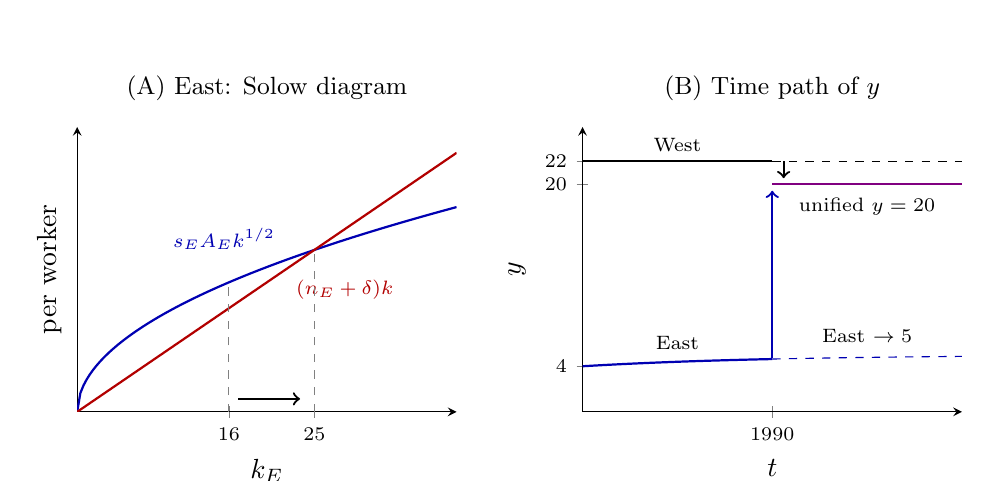
\begin{tikzpicture}
\begin{axis}[name=solow,width=6.4cm,height=5.2cm,axis lines=left,xmin=0,xmax=40,ymin=0,ymax=3.3,
  xlabel={$k_E$},ylabel={per worker},xtick={16,25},
  ytick=\empty,title={\small (A) East: Solow diagram},every tick label/.append style={font=\scriptsize}]
\addplot[domain=0:40,samples=120,thick,blue!70!black]{0.375*sqrt(x)} node[pos=0.55,above left,font=\scriptsize]{$s_EA_Ek^{1/2}$};
\addplot[domain=0:40,thick,red!70!black]{0.075*x} node[pos=0.55,below right,font=\scriptsize]{$(n_E+\delta)k$};
\draw[dashed,gray](axis cs:16,0)--(axis cs:16,1.5);
\draw[dashed,gray](axis cs:25,0)--(axis cs:25,1.875);
\draw[->,thick](axis cs:17,0.15)--(axis cs:23.5,0.15);
\end{axis}
\begin{axis}[at={(solow.east)},anchor=west,xshift=1.6cm,width=6.4cm,height=5.2cm,axis lines=left,
  xmin=-10,xmax=10,ymin=0,ymax=25,xlabel={$t$},ylabel={$y$},xtick={0},xticklabels={1990},
  ytick={4,20,22},title={\small (B) Time path of $y$},every tick label/.append style={font=\scriptsize}]
\addplot[thick,black]coordinates{(-10,22)(0,22)};
\addplot[dashed,black]coordinates{(0,22)(10,22)};
\addplot[domain=-10:0,samples=40,thick,blue!70!black]{5-exp(-0.1*(x+10))};
\addplot[domain=0:10,samples=40,dashed,blue!70!black]{5-exp(-0.1*(x+10))};
\addplot[thick,violet]coordinates{(0,20)(10,20)};
\draw[->,thick,blue!70!black](axis cs:0,4.7)--(axis cs:0,19.4);
\draw[->,thick,black](axis cs:0.6,22)--(axis cs:0.6,20.5);
\node[font=\scriptsize,anchor=south] at (axis cs:-5,22){West};
\node[font=\scriptsize,anchor=south] at (axis cs:-5,4.6){East};
\node[font=\scriptsize,anchor=south] at (axis cs:5,5.2){East $\to5$};
\node[font=\scriptsize,anchor=north] at (axis cs:5,19.6){unified $y=20$};
\end{axis}
\end{tikzpicture}\\
{\footnotesize Figure 1. (A) East starts below its own $k^*$. (B) Solid: actual paths; dashed: no-unification counterfactuals (schematic timing).}
\end{center}
\rubric{
\item Period-0 values: 1 pt. Steady-state formula and four numbers: 2 pts.
\item Direction for each region (West flat, East rising with falling growth): 1 pt.
\item Named \emph{conditional} convergence, gap in levels persists: 1 pt. Diagram with labelled curves, $k_0$, $k^*$: counts in this point if the words are missing.
\item Calling it ``divergence'' or ``absolute convergence'': max.\ 2 pts.
}
\end{sol}

\textbf{b)} (5 points) Unification: from 1990 all production uses West technology $A_W=2$ with the
pooled capital and labour of both regions. Compute the new $y$ and its change for West and for East
workers (in levels and in \% of the pre-unification value), and the change in aggregate German output
$Y$. Explain \emph{where} each region's gain or loss comes from.
\answerspace
\begin{sol}
\step{pooling}{$K=7744+256=8000$, $L=64+16=80\Rightarrow k_U=8000/80=100$, $y_U=2\sqrt{100}=\res{20}$.}
\step{per capita changes}{West: $22\to20$: $\res{-2,\ -9.09\%}$ (base 22). East: $4\to20$: $\res{+16,\ +400\%}$ (base 4).}
\step{West: source}{\textbf{Capital dilution}: same $A$, but $k$: $121\to100$ because East brings 20\% of the workers
and only 3.2\% of the capital. $K/L\downarrow\to y\downarrow$. Factor prices: $w=(1-\alpha)y$: $11\to10$ (West workers lose);
$r^K=\alpha y/k$: $1/11=0.091\to0.10$ (West capital owners gain).}
\step{East: source}{\textbf{Technology} $A:1\to2$ and \textbf{capital deepening} $k:16\to100$. Technology first:
$1\cdot4\to2\cdot4=8$ ($+4$), then capital $8\to20$ ($+12$). In logs (order-free):
$\ln5=\underbrace{\ln2}_{\text{technology}}+\underbrace{\tfrac12\ln(100/16)}_{\text{capital deepening}}=0.693+0.916$;
technology $\approx43\%$ of the log gain. $w_E$: $2\to10$.}
\step{aggregate}{Before: $Y=22\cdot64+4\cdot16=1408+64=1472$. After: $Y=20\cdot80=1600$.
$\Delta Y=\res{+128,\ +8.70\%}$. Germany-wide $y$: $1472/80=18.4\to20$. Source: East's $K$ and $L$ now work
with the better technology; West's loss per head is a \emph{redistribution} of capital, not lost output.}
\step{check}{$64\cdot(-2)+16\cdot(+16)=-128+256=128=\Delta Y$.}
\intuition{Per-capita and aggregate answers differ in sign for the West: West $y$ falls, yet German $Y$ rises.
``Not per capita for the West, but still an aggregate gain.''}
\refbib{Kurlat \S4.1--\S4.2, pp.~53--61; \S4.4, pp.~63--69 (factor prices).}
\rubric{
\item $k_U$, $y_U$ and the two per-capita changes with bases: 2 pts.
\item Sources: West = capital dilution (1 pt); East = technology + capital deepening (1 pt).
\item Aggregate $\Delta Y$ computed and interpreted: 1 pt.
\item Numbers with no source of gain/loss: max.\ 3 pts. Per capita only, no aggregate: max.\ 4 pts. Arithmetic slip: $-1$.
}
\end{sol}

\textbf{c)} (5 points) After unification Germany saves at the West's rate $s_W$ and its labour force
grows at the labour-weighted average of $n_W$ and $n_E$. Compute $k^*_U$ and $y^*_U$. Is unified
Germany below its steady state? Compare $y^*_U$ with $y^*_W$ and explain the difference.
\answerspace
\begin{sol}
\step{population growth}{$n_U=\dfrac{64\cdot0+16\cdot0.025}{80}=\dfrac{0.4}{80}=0.005$.}
\step{steady state}{$\dfrac{s_WA_W}{n_U+\delta}=\dfrac{0.55}{0.055}=10\Rightarrow\res{k^*_U=100,\ y^*_U=20}$.}
\step{position}{$k_U=100=k^*_U$: \res{\text{exactly at the steady state}} --- no transition; $y$ stays at 20,
$g_y=0$, and aggregate $Y$ grows at $n_U=0.5\%$.}
\step{comparison}{$y^*_U=20<y^*_W=22$ although $A$ and $s$ are the West's. The only difference is
$n_U=0.005>n_W=0$: break-even investment $(n+\delta)k$ is steeper ($0.055$ vs $0.05$), so each worker's capital
is diluted faster by newcomers and the same saving supports less $k$:
$n\uparrow\to(n+\delta)k\uparrow\to k^*\downarrow\to y^*\downarrow$.}
\intuition{Unification did not make the West's steady state unattainable because of the East's technology
(that was replaced) or its saving (not used): it is population growth alone. The 2-point gap is permanent,
unlike the 2-point loss in (b), which was a pure level redistribution.}
\refbib{Kurlat \S4.2, pp.~59--61; \S5.3, pp.~79--86 (convergence).}
\rubric{
\item $n_U$: 1 pt. $k^*_U$, $y^*_U$: 2 pts.
\item Position relative to SS: 1 pt. Explanation via $n$ and break-even investment: 1 pt.
\item Numbers with no explanation: max.\ 3 pts. Using unweighted $n$ ($0.0125$): $-1$ pt, rest graded on method.
}
\end{sol}
\begin{sol}
\gap{Lista 2, 1(b) (``divergence'' instead of conditional convergence); 1(c) (source of each region's gain/loss); 1(d) (numbers right, no explanation).}
\end{sol}

% =============================================================================
\block{III}{Microfoundations}{Lectures 4--6; Kurlat chs.~6, 7, 9 \,\textbullet\, 25 points}

\question{(10 points) Objective items.}

\textbf{a)} (3 points) A household has one unit of time, preferences $\ln c+\psi\ln l$ with $\psi=1$,
wage $w=10$, pays a tax $\tau$ on labour income and receives a lump-sum transfer $T=2$, so
$c=(1-\tau)w(1-l)+T$. The labour-income tax rises from $\tau=0.2$ to $\tau=0.5$ ($T$ unchanged). Hours:
\begin{options}
\item fall from 0.375 to 0.300: leisure became cheaper, an effect that would lower hours even with $T=0$.
\item stay at 0.500: with log utility the income and substitution effects cancel whatever $T$ is.
\item rise from 0.375 to 0.450: the lower net wage makes the household poorer, so it works more.
\item fall from 0.500 to 0.375: the tax lowers the price of leisure one-for-one with $\tau$.
\item fall from 0.375 to 0.300: the fixed $T$ grows relative to net earnings; with $T=0$ hours would not move.
\end{options}
\answer{E}
\begin{sol}
\step{labour supply}{MRS $=$ net wage: $\dfrac{\psi c}{l}=(1-\tau)w$ with $c=(1-\tau)w(1-l)+T$ $\Rightarrow$
$n=1-l=\dfrac{1}{1+\psi}-\dfrac{\psi T}{(1+\psi)(1-\tau)w}$. $\tau=0.2$: $0.5-\frac{2}{16}=0.375$; $\tau=0.5$: $0.5-\frac{2}{10}=0.300$.
With $T=0$, $n=0.5$ for any $\tau$: the effect runs only through $T$ (pure income effect), so A's reason is false.}
\refbib{Kurlat \S7.2, pp.~131--137.}
\gap{Lista 4, 1(b): the words described a substitution effect; the formula said the effect is through $T$.}
\end{sol}

\medskip
\textbf{b)} (3 points) In a search economy with $m(V,U)=\mu V^\alpha U^{1-\alpha}$, one firm posts one extra
vacancy. Which statement is correct?
\begin{options}
\item The posting firm and the other firms gain; unemployed workers lose, as matches per worker fall.
\item Unemployed workers gain ($f$ rises); other firms lose ($q$ falls); the posting firm gains privately.
\item The posting firm loses, because its own $q$ falls; this private cost is the congestion externality.
\item Everyone gains, since $m$ rises one-for-one with $V$, so the extra vacancy creates no externality.
\item Unemployed workers lose ($f$ falls); other firms gain ($q$ rises); the posting firm is unaffected.
\end{options}
\answer{B}
\begin{sol}
\step{signs}{$\theta=V/U\uparrow\Rightarrow f=\mu\theta^\alpha\uparrow$, $q=\mu\theta^{\alpha-1}\downarrow$; $\partial m/\partial V=\alpha q<q$
(not one-for-one: friction). The congestion cost lands on \emph{other} firms; the posting firm, which
expects profit, ignores both that cost and the benefit to workers.}
\refbib{Kurlat \S7.5, pp.~142--150.}
\gap{Lista 4, 2(d): externality placed on the posting firm itself.}
\end{sol}

\medskip
\textbf{c)} (2 points, T or F) A fall in matching efficiency $\mu$, which raises the vacancy rate
needed at every unemployment rate, is a movement along the Beveridge curve.
\answer{False}
\begin{sol}
\step{shift}{The Beveridge curve $s(1-u)=\mu v^\alpha u^{1-\alpha}$ (job destruction $=$ job creation) is drawn for a given
$\mu$. $\mu\downarrow$ moves every $(u,v)$ pair out: a \emph{shift}. A movement along it is a change in
tightness $\theta$ at given matching technology.}
\refbib{Kurlat \S7.1, pp.~127--131; \S7.5.}
\gap{Lista 4, 2(e): shift of vs movement along the Beveridge curve.}
\end{sol}

\medskip
\textbf{d)} (2 points, T or F) In the general-equilibrium economy with a fixed capital stock, no
investment, and preferences $\ln c+\psi\ln l$, a rise in TFP $A$ leaves hours worked unchanged.
\answer{True}
\begin{sol}
\step{equilibrium}{$\psi c/l=w$, $c=Y=AK^\alpha L^{1-\alpha}$, $w=(1-\alpha)AK^\alpha L^{-\alpha}$ $\Rightarrow$
$\psi\frac{L}{1-L}=1-\alpha\Rightarrow L=\frac{1-\alpha}{1-\alpha+\psi}$: no $A$. Equivalently
$\frac{d\ln L}{d\ln A}=\frac{1-\sigma}{\cdots}=0$ at $\sigma=1$: income and substitution effects cancel.}
\refbib{Kurlat \S9.1, pp.~165--168.}
\gap{Lista 5 (ungraded) and Lista 4, 1(b): with log utility, wage changes alone do not move hours.}
\end{sol}

% -----------------------------------------------------------------------------
\question{(15 points) A temporary tax cut financed by public debt. The Brazilian government
considers cutting this year's income tax and repaying the resulting debt next period. A household lives
two periods and solves
\[
\max_{c_1,c_2,a}\ u(c_1)+\beta u(c_2)\quad\text{s.t.}\quad c_1+a=y_1-\tau_1,\qquad c_2=y_2-\tau_2+(1+r)a,
\]
with $u(c)=\frac{c^{1-\sigma}}{1-\sigma}$ ($u=\ln c$ if $\sigma=1$), $\beta\in(0,1)$, $\sigma>0$. Baseline values:
$\sigma=1$, $\beta=0.8$, $r=0.25$ (a period is roughly a decade), $y_1=60$, $y_2=150$, $\tau_1=\tau_2=20$ (thousand reais).}

\textbf{a)} (5 points) By substituting the constraints into the objective (no Lagrangian needed), derive
the Euler equation and solve for $c_1$, $c_2$ and $a$ in closed form. Evaluate them at the baseline.
\answerspace
\begin{sol}
\step{substitute}{From period 1: $a=y_1-\tau_1-c_1$. Into period 2: $c_2=y_2-\tau_2+(1+r)(y_1-\tau_1-c_1)$.
Dividing by $1+r$: $c_1+\dfrac{c_2}{1+r}=\underbrace{y_1-\tau_1+\dfrac{y_2-\tau_2}{1+r}}_{\equiv\,W\ \text{(PV of after-tax income)}}$.}
\step{FOC}{$\max_{c_1}\ u(c_1)+\beta u\big(y_2-\tau_2+(1+r)(y_1-\tau_1-c_1)\big)$:\quad
$u'(c_1)-\beta(1+r)u'(c_2)=0\Rightarrow\res{c_1^{-\sigma}=\beta(1+r)\,c_2^{-\sigma}}$ (Euler: MRS $=1+r$).}
\step{solve}{$c_2=[\beta(1+r)]^{1/\sigma}c_1$. Into the PV constraint: $c_1\left[1+\beta^{1/\sigma}(1+r)^{\frac1\sigma-1}\right]=W$:
\[
\res{c_1=\frac{W}{D}},\quad \res{c_2=[\beta(1+r)]^{1/\sigma}\frac{W}{D}},\quad \res{a=y_1-\tau_1-\frac{W}{D}},\qquad
D\equiv1+\beta^{1/\sigma}(1+r)^{\frac1\sigma-1}.
\]}
\step{baseline}{$W=40+\frac{130}{1.25}=40+104=144$; $\sigma=1\Rightarrow D=1+\beta=1.8$.
$c_1=144/1.8=\res{80}$; $c_2=(0.8\cdot1.25)\cdot80=\res{80}$; $a=40-80=\res{-40}$ (borrows).}
\step{check}{$c_2=130+1.25\cdot(-40)=130-50=80$ \checkmark; Euler $1/80=0.8\cdot1.25/80$ \checkmark.}
\rubric{
\item Substitution and PV constraint: 1 pt. Euler equation: 1 pt.
\item Closed forms for $c_1,c_2$: 1 pt; \textbf{$a$ solved}: 1 pt. Baseline numbers: 1 pt.
\item Not solving for $a$: max.\ 4 pts. Lagrangian route is accepted. Arithmetic slip: $-1$.
}
\end{sol}

\textbf{b)} (5 points) Set $y_2=\tau_1=\tau_2=0$ (general $\sigma$). Compute $\partial c_1/\partial r$, isolate
the factor that determines its sign, and state, in words consistent with that sign, what happens to
$c_1$ when $r$ rises for $\sigma>1$, $\sigma=1$ and $\sigma<1$.
\answerspace
\begin{sol}
\step{set up}{$W=y_1$, so $c_1=\dfrac{y_1}{D(r)}$, $D(r)=1+\beta^{1/\sigma}(1+r)^{\frac{1-\sigma}{\sigma}}$.}
\step{differentiate}{$\dfrac{\partial D}{\partial r}=\beta^{1/\sigma}\,\dfrac{1-\sigma}{\sigma}\,(1+r)^{\frac{1-2\sigma}{\sigma}}$, so
\[
\frac{\partial c_1}{\partial r}=-\frac{y_1}{D^2}\frac{\partial D}{\partial r}
=\frac{y_1\,\beta^{1/\sigma}(1+r)^{\frac{1-2\sigma}{\sigma}}}{D^2}\cdot\underbrace{\frac{\sigma-1}{\sigma}}_{\text{determines the sign}}.
\]}
\step{sign}{$\res{\sigma>1:\ \partial c_1/\partial r>0}$;\quad $\res{\sigma=1:\ =0}$ ($c_1=y_1/(1+\beta)$);\quad $\res{\sigma<1:\ <0}$.}
\step{words}{The household is a pure saver. $r\uparrow$: \emph{substitution effect} --- $c_1$ is dearer in units of
$c_2$ $\to c_1\downarrow$; \emph{income effect} --- a saver is richer $\to c_1\uparrow$. $\sigma$ is the curvature of $u$;
$1/\sigma$ is the elasticity of intertemporal substitution. $\sigma>1$ (low EIS): income effect dominates,
so $c_1$ \textbf{rises} and saving falls. $\sigma<1$: substitution dominates, $c_1$ \textbf{falls}. $\sigma=1$: they cancel.}
\refbib{Kurlat \S6.2, pp.~112--115.}
\rubric{
\item $c_1(r)$ and correct derivative: 2 pts. Sign factor isolated: 1 pt.
\item Words matching the sign for each case (income vs substitution, saver): 2 pts.
\item Correct sign condition but words with the opposite direction (e.g.\ ``$\sigma>1$, $c_1$ falls''): max.\ 2 pts.
}
\end{sol}

\textbf{c)} (5 points) Return to the baseline. The government cuts $\tau_1$ by $\Delta=10$ and raises
$\tau_2$ by $(1+r)\Delta$. (i) Find the effect on $c_1$, $c_2$ and $a$. Does the timing of taxes matter?
(ii) Now the household faces a borrowing limit $a\ge-b$ with $b=20$. Find $c_1$, $c_2$, $a$ before and
after the same tax change. (iii) Give two concrete examples of Brazilian households for whom such a
limit is likely to bind.
\answerspace
\begin{sol}
\step{(i) PV of taxes}{$\tau_1'+\dfrac{\tau_2'}{1+r}=(\tau_1-\Delta)+\dfrac{\tau_2+(1+r)\Delta}{1+r}=\tau_1+\dfrac{\tau_2}{1+r}=36$:
$W$ unchanged $\Rightarrow$ $\res{\Delta c_1=\Delta c_2=0,\ \Delta a=+\Delta=+10}$.
Numbers: $\tau_1=10$, $\tau_2=20+12.5=32.5$; $W=50+117.5/1.25=50+94=144$; $c_1=c_2=80$; $a=50-80=-30$.
The household saves the whole cut to pay the future tax (Ricardian equivalence): \textbf{timing does not
matter}, only the PV of taxes.}
\step{(ii) before}{Desired $a=-40<-20$ $\Rightarrow$ limit binds: $a=-20$, $c_1=y_1-\tau_1+b=40+20=\res{60}$,
$c_2=130+1.25(-20)=130-25=\res{105}$. Euler becomes an inequality: $u'(c_1)=1/60>\beta(1+r)u'(c_2)=1/105$.}
\step{(ii) after}{Desired $a=-30<-20$: still binds. $a=-20$; $c_1=50+20=\res{70}$ ($+10=\Delta$);
$c_2=117.5-25=\res{92.5}$ ($-12.5=-(1+r)\Delta$). MPC out of the cut $=1$; timing \textbf{matters}.
(It keeps binding while $-40+\Delta<-20$, i.e.\ $\Delta<20$.)}
\step{(iii) examples}{(1) A young medical resident or university student with low income now and high
expected income later, and no collateral. (2) An informal worker (or someone with a negative record at
Serasa) whose income fell temporarily and who cannot borrow against future earnings.}
\begin{center}
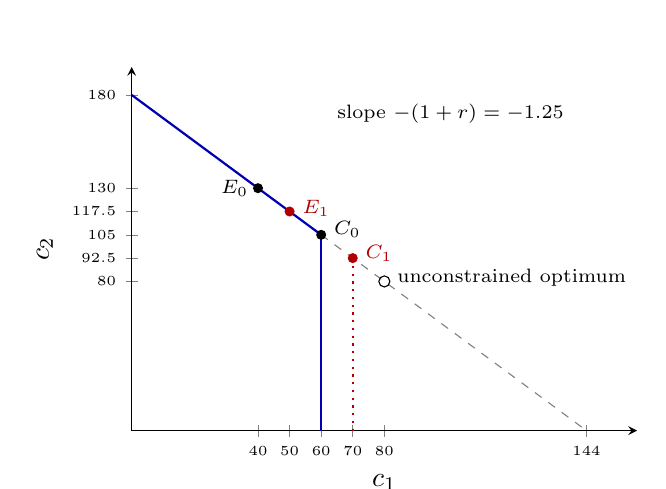
\begin{tikzpicture}
\begin{axis}[width=8cm,height=6.2cm,axis lines=left,xmin=0,xmax=160,ymin=0,ymax=195,
  xlabel={$c_1$},ylabel={$c_2$},xtick={40,50,60,70,80,144},ytick={80,92.5,105,117.5,130,180},
  every tick label/.append style={font=\tiny}]
\addplot[domain=60:144,dashed,gray]{1.25*(144-x)};
\addplot[domain=0:60,thick,blue!70!black]{1.25*(144-x)};
\draw[thick,blue!70!black](axis cs:60,105)--(axis cs:60,0);
\draw[dotted,thick,red!70!black](axis cs:70,92.5)--(axis cs:70,0);
\addplot[only marks,mark=*,mark size=1.6pt]coordinates{(40,130)(60,105)};
\addplot[only marks,mark=*,mark size=1.6pt,red!70!black]coordinates{(50,117.5)(70,92.5)};
\addplot[only marks,mark=o,mark size=2pt]coordinates{(80,80)};
\node[font=\scriptsize,anchor=east] at (axis cs:40,130){$E_0$};
\node[font=\scriptsize,anchor=west,red!70!black] at (axis cs:51,119){$E_1$};
\node[font=\scriptsize,anchor=west] at (axis cs:61,108){$C_0$};
\node[font=\scriptsize,anchor=west,red!70!black] at (axis cs:71,95){$C_1$};
\node[font=\scriptsize,anchor=west] at (axis cs:81,82){unconstrained optimum};
\node[font=\scriptsize,anchor=west] at (axis cs:62,170){slope $-(1+r)=-1.25$};
\end{axis}
\end{tikzpicture}\\
{\footnotesize Figure 2. The budget line is the same before and after the swap ($W=144$); the endowment slides
from $E_0$ to $E_1$ along it. The limit $c_1\le y_1-\tau_1+b$ moves from 60 to 70, so the constrained choice moves
from $C_0$ to $C_1$.}
\end{center}
\intuition{Ricardian equivalence needs the household to be able to move resources across periods at $r$.
When the limit binds, the tax cut is the loan the market would not give, and it is consumed one-for-one.}
\refbib{Kurlat \S6.2--\S6.4, pp.~120--126.}
\rubric{
\item (i) PV argument and $\Delta c_1=\Delta c_2=0$, $\Delta a=\Delta$: 2 pts.
\item (ii) Binding check and $c_1$ before/after: 1.5 pts (diagram with kink, labelled axes and points counts here).
\item (iii) Two examples: 1.5 pts (0.75 each).
\item Proving PV-only and then stating ``timing matters'' in the unconstrained case: max.\ 2 pts. One example only: $-0.75$.
}
\end{sol}
\begin{sol}
\gap{Lista 3, 1(a)(d) (never solved for $a$); 1(c) (right sign condition, opposite words); 1(e) (PV proved, then ``timing matters''); 2(b) (one example where two were asked).}
\end{sol}

% =============================================================================
\block{IV}{Money, inflation and AD--AS}{Lectures 7--9; Kurlat chs.~10--11; Benigno (2015) \,\textbullet\, 25 points}

\question{(10 points) Objective items.}

\textbf{a)} (3 points) About the quantity equation $MV=PY$:
\begin{options}
\item It is a theory of money demand: with $Y$ fixed, doubling $M$ doubles $P$ at every horizon.
\item It is an identity which proves neutrality, because $V$ and $Y$ are constant by definition.
\item It is a behavioural equation: $V$ is a structural parameter that the central bank sets.
\item It is an identity, since $V\equiv PY/M$; causation needs assumptions on $V$ and on what is exogenous.
\item It is an identity which proves causation runs from $P$ to $M$, because firms set prices first.
\end{options}
\answer{D}
\begin{sol}
\step{residual}{$V$ is measured as $PY/M$, so the equation holds for any data. It becomes a theory only with
an assumption on $V$ (e.g.\ stable, or given by a money-demand model) and on which variable is exogenous.}
\refbib{Kurlat \S10.4, pp.~199--204; \S11.2.}
\gap{Lista 6, 1(a): $V$ as a residual; causation needs an assumption.}
\end{sol}

\medskip
\textbf{b)} (3 points) In steady state with constant $i$, $\pi=\mu-\eta g$. The central bank targets $\pi^*=3\%$
with $g=2\%$ and sets $\mu$ assuming $\eta=1$ (Cambridge). Money demand is actually Baumol--Tobin. Inflation is:
\begin{options}
\item $2\%$
\item $3\%$
\item $4\%$
\item $5\%$
\item $6\%$
\end{options}
\answer{C}
\begin{sol}
\step{compute}{Chosen $\mu=\pi^*+1\cdot g=5\%$. Baumol--Tobin: $\eta=\tfrac12$, so $\pi=5\%-\tfrac12\cdot2\%=\res{4\%}$.
Desired real balances grow at $1\%$, not $2\%$: the extra money goes into prices.}
\refbib{Kurlat \S11.2, pp.~205--215.}
\gap{Lista 6, 2(b): inflation-targeting error formula.}
\end{sol}

\medskip
\textbf{c)} (2 points, T or F) When the central bank targets the nominal interest rate, the money-market
equilibrium $M=p\,m^D(Y,i)$ determines the quantity of money.
\answer{True}
\begin{sol}
\step{endogenous $M$}{With $i$ fixed by policy, and $p$, $Y$ given, $M$ must supply whatever $p\,m^D(Y,i)$ demands: the
central bank accommodates by open-market operations. Under a money target it is the reverse: $M$ given, $i$ adjusts.}
\refbib{Kurlat \S11.1--\S11.2; Benigno \S3 (policy sets $i$).}
\gap{Lista 6, 1(d): under an interest-rate target the money market determines $M$.}
\end{sol}

\medskip
\textbf{d)} (2 points, T or F) In Benigno's AD--AS model, a temporary rise in firms' desired mark-up
shifts the AD curve to the left.
\answer{False}
\begin{sol}
\step{which curve}{The mark-up enters the price-setting (AS) block: natural output falls, AS shifts up/left. AD comes
from the Euler equation and the policy rule, where $\mu$ does not appear: AD does not move (stagflation along AD).}
\refbib{Benigno (2015) \S4 and \S7.}
\gap{Shift of vs movement along AD/AS (taxonomy).}
\end{sol}

% -----------------------------------------------------------------------------
\question{(15 points) Pix and the demand for money. Since 2020 Pix, Brazil's instant-payment
system, has lowered the cost of turning deposits into means of payment. Model real money demand with
Baumol--Tobin, $m^D=\sqrt{\dfrac{FY}{2i}}$, where $F$ is the real cost of each conversion. Assume real
output grows at $g=2\%$, $F$ falls at the constant rate $\dot F/F=f=-4\%$, and $i$ is constant. The
money market clears: $M=p\,m^D(Y,i,F)$.}

\textbf{a)} (5 points) Derive velocity $V$ implied by this model. Explain why $V$ is not constant, and
compute its growth rate under the assumptions above. Interpret velocity in words.
\answerspace
\begin{sol}
\step{definition}{$V\equiv\dfrac{pY}{M}=\dfrac{pY}{p\,m^D}=\dfrac{Y}{\sqrt{FY/2i}}=\res{\sqrt{\dfrac{2iY}{F}}}$.}
\step{not constant}{$V$ depends on $i$ (opportunity cost of holding money $\uparrow\Rightarrow V\uparrow$), on $Y$
(economies of scale in cash management, $\partial\ln V/\partial\ln Y=\tfrac12$) and on $F$ (payment technology,
$\partial\ln V/\partial\ln F=-\tfrac12$).}
\step{growth}{$\dfrac{\dot V}{V}=\tfrac12\dfrac{\dot i}{i}+\tfrac12 g-\tfrac12 f=0+1\%+2\%=\res{3\%\ \text{per year}}$.}
\step{interpret}{$V$ is the number of times the average real balance is spent per period. In $MV=PY$ it
is a residual; Baumol--Tobin gives it a theory: cheaper conversions $\to$ smaller average balances per real
transaction $\to$ each real balance turns over faster.}
\refbib{Kurlat \S10.4, pp.~199--204.}
\rubric{
\item $V=\sqrt{2iY/F}$ derived: 2 pts.
\item Dependence on $i$, $Y$, $F$ with signs: 1 pt. Growth $3\%$: 1 pt. Interpretation: 1 pt.
\item Treating $V$ as constant or exogenous: max.\ 2 pts.
}
\end{sol}

\textbf{b)} (5 points) By totally differentiating $M=p\,m^D(Y,i,F)$ with respect to time, show that in
steady state $\pi=\mu-\tfrac12(g+f)$. Before Pix ($f=0$) the BCB grew money at the rate that delivered
$\pi=3\%$. Which money growth $\mu$ delivers $3\%$ after Pix? What inflation results if the BCB keeps the
old $\mu$? Explain the mechanism in words.
\answerspace
\begin{sol}
\step{differentiate}{$\dot M=\dot p\,m^D+p\left[\dfrac{\partial m^D}{\partial Y}\dot Y+\underbrace{\dfrac{\partial m^D}{\partial i}\dot i}_{=0\ (i\ \text{const.})}+\dfrac{\partial m^D}{\partial F}\dot F\right]$.}
\step{divide by $M=p\,m^D$}{$\mu=\pi+\underbrace{\dfrac{\partial m^D}{\partial Y}\dfrac{Y}{m^D}}_{\eta_Y}g+\underbrace{\dfrac{\partial m^D}{\partial F}\dfrac{F}{m^D}}_{\eta_F}f$.
From $m^D=(FY/2i)^{1/2}$: $\eta_Y=\eta_F=\tfrac12$ $\Rightarrow$ $\res{\pi=\mu-\tfrac12(g+f)}$.}
\step{before Pix}{$f=0$: $\mu=\pi^*+\tfrac12g=3\%+1\%=4\%$.}
\step{after Pix}{$\mu=\pi^*+\tfrac12(g+f)=3\%+\tfrac12(2\%-4\%)=3\%-1\%=\res{2\%}$.
Keeping $\mu=4\%$: $\pi=4\%-\tfrac12(-2\%)=\res{5\%}$.}
\step{mechanism}{$F\downarrow\to$ households hold smaller real balances $\to$ desired real money grows at
$\tfrac12(g+f)=-1\%$ instead of $+1\%$ $\to$ the same $\mu=4\%$ chases a \emph{shrinking} demand for real balances
$\to$ excess money $\to p$ grows faster: $\pi=5\%$. Equivalently, velocity rises at $3\%$. It is lower money
\emph{demand}, not ``cheap money''.}
\refbib{Kurlat \S11.2, pp.~205--215.}
\rubric{
\item Total differentiation with $\dot i=0$ struck: 1 pt. Elasticities named and $=\tfrac12$: 1 pt.
\item $\mu=2\%$ and $\pi=5\%$: 2 pts (1 each). Mechanism via money demand/velocity: 1 pt.
\item Explaining the effect as ``cheaper money'' or ``more money supply'': max.\ 3 pts. Arithmetic slip: $-1$.
}
\end{sol}

\textbf{c)} (5 points) Suppose instead the BCB sets the Selic (an interest-rate target $i^*$) and lets the
money supply be whatever it must be. When Pix lowers $F$, what adjusts in the money market in the short
run (prices sticky)? Is the Pix effect inflationary under this regime in the long run? Contrast with the
money-growth rule of (b).
\answerspace
\begin{sol}
\step{short run}{$F\downarrow\Rightarrow m^D\downarrow$ at every $i$ (curve shifts left). If $M$ stayed put, excess money
would push $i$ below $i^*$. To hold $i=i^*$ the BCB drains money (sells bonds):
$F\downarrow\to m^D\downarrow\to$ BCB sells bonds $\to M\downarrow$, $i=i^*$ unchanged $\to$ AD unchanged $\to y,p$ unchanged.
\res{\text{$M$ adjusts; $i$ does not.}}}
\step{long run}{$\pi$ is pinned by the target: $\pi=3\%$. Money growth becomes endogenous:
$\mu=\pi+\tfrac12(g+f)=3\%+\tfrac12(2\%-4\%)=\res{2\%}$. \res{\text{Not inflationary}}; Pix shows up only as slower
growth of money aggregates and rising velocity.}
\step{contrast}{Under a money-growth rule ($\mu=4\%$ fixed) the same shock raises $\pi$ to $5\%$, as in (b). The regime
decides whether a money-demand shock reaches prices: with an $i$ target the central bank absorbs it.}
\begin{center}
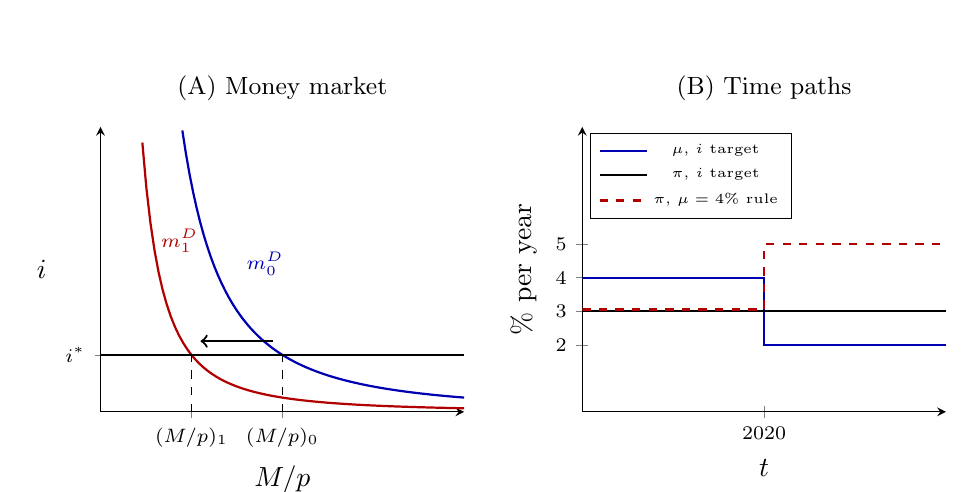
\begin{tikzpicture}
\begin{axis}[name=mm,width=6.2cm,height=5.2cm,axis lines=left,xmin=0,xmax=4,ymin=0,ymax=2.5,
  xlabel={$M/p$},ylabel={$i$},xtick={1,2},xticklabels={$(M/p)_1$,$(M/p)_0$},ylabel style={rotate=-90},ytick={0.5},yticklabels={$i^*$},
  title={\small (A) Money market},every tick label/.append style={font=\scriptsize}]
\addplot[domain=0.9:4,samples=80,thick,blue!70!black]{2/x^2};
\node[font=\scriptsize,blue!70!black,anchor=west] at (axis cs:1.5,1.3){$m^D_0$};
\addplot[domain=0.46:4,samples=80,thick,red!70!black]{0.5/x^2};
\node[font=\scriptsize,red!70!black] at (axis cs:0.87,1.5){$m^D_1$};
\addplot[thick,black]coordinates{(0,0.5)(4,0.5)};
\draw[dashed](axis cs:2,0)--(axis cs:2,0.5);
\draw[dashed](axis cs:1,0)--(axis cs:1,0.5);
\draw[->,thick](axis cs:1.9,0.62)--(axis cs:1.1,0.62);
\end{axis}
\begin{axis}[at={(mm.east)},anchor=west,xshift=1.5cm,width=6.2cm,height=5.2cm,axis lines=left,
  xmin=-5,xmax=5,ymin=0,ymax=8.5,xlabel={$t$},ylabel={\% per year},xtick={0},xticklabels={2020},
  ytick={2,3,4,5},title={\small (B) Time paths},every tick label/.append style={font=\scriptsize},
  legend style={font=\tiny,at={(0.02,0.98)},anchor=north west}]
\addplot[thick,blue!70!black]coordinates{(-5,4)(0,4)(0,2)(5,2)};
\addlegendentry{$\mu$, $i$ target}
\addplot[thick,black]coordinates{(-5,3)(5,3)};
\addlegendentry{$\pi$, $i$ target}
\addplot[dashed,thick,red!70!black]coordinates{(-5,3.05)(0,3.05)(0,5)(5,5)};
\addlegendentry{$\pi$, $\mu=4\%$ rule}
\end{axis}
\end{tikzpicture}\\
{\footnotesize Figure 3. (A) Lower $F$ shifts money demand left from $m^D_0=m^D(F_0)$ to $m^D_1=m^D(F_1)$ (drawn for $F_1=F_0/4$, which halves $m^D$); at $i^*$ real balances fall from $(M/p)_0$ to $(M/p)_1$.
(B) Under the $i$ target $\mu$ falls from 4\% to 2\% and $\pi$ stays at 3\%; under a fixed $\mu=4\%$, $\pi$ rises to 5\%.}
\end{center}
\intuition{Money is endogenous under an interest-rate rule: the central bank supplies the money people want at $i^*$.
A payment innovation that lowers money demand therefore changes $M$, not $i$, and leaves AD and inflation alone.}
\refbib{Kurlat \S11.1--\S11.2, pp.~205--215; Benigno (2015) \S3 (the central bank sets $i$).}
\rubric{
\item Short run: $m^D$ shifts left, $M$ adjusts, $i$ unchanged, no AD effect: 2 pts (arrow chain or diagram with labelled axes, curves and shift direction).
\item Long run: $\pi$ anchored, $\mu$ endogenous $=2\%$: 2 pts. Contrast with the money rule: 1 pt.
\item Stating that the BCB keeps $M$ fixed (or that $i$ falls) under an $i$ target: max.\ 2 pts.
}
\end{sol}
\begin{sol}
\gap{Lista 6, 1(a)(b) ($V$ a residual, velocity interpreted); 1(c) (mechanism; flexible-price neutrality: in the long run only $\pi$ and nominal aggregates move); 1(d) ($M$ endogenous under an $i$ target); 2(c) (falling $F$ = lower money demand, not ``cheap money'').}
\end{sol}

\end{document}
"
% Check fonts afterwards: pdffonts simulado-01-solutions.pdf  (all Type 1)
% Every number in the key is verified by simulado_codigo/check_simulado_01.py
% =============================================================================
\documentclass[11pt,a4paper]{article}
\usepackage[utf8]{inputenc}
\usepackage[T1]{fontenc}
\usepackage{lmodern}   % Type 1 vector fonts (replaces PK bitmaps)
\usepackage{cmap}      % ToUnicode CMap -> copyable text
\usepackage[english]{babel}
\usepackage{amsmath,amssymb,amsfonts}
\usepackage[a4paper,margin=2.2cm]{geometry}
\usepackage{enumitem}
\usepackage{fancyhdr}
\usepackage{comment}
\def\CommentCutFile{simulado-01.cut} % private cut file: sibling sources build in this folder
\usepackage{xcolor}
\usepackage{booktabs}
\usepackage{microtype}
\usepackage{pgfplots}
\pgfplotsset{compat=1.16}

% ====================== CONFIGURATION ======================
\newif\ifsolucoes
\ifdefined\withsolutions\solucoestrue\else\solucoesfalse\fi

\newcommand{\course}{Macroeconomics I --- MPE Insper}
\newcommand{\examtitle}{Mock Final Exam 1 (Simulado 1)}
\newcommand{\answerheight}{5.2cm}

% ====================== MACHINERY ======================
\ifsolucoes\includecomment{sol}\else\excludecomment{sol}\fi

\pagestyle{fancy}\fancyhf{}
\lhead{\footnotesize\course}
\rhead{\footnotesize\examtitle\ifsolucoes{} --- Solutions and Rubric\fi}
\cfoot{\footnotesize\thepage}
\renewcommand{\headrulewidth}{0.3pt}
\setlength{\headheight}{14pt}

\setlist{topsep=2pt,itemsep=2pt}
\newcounter{questao}

\newcommand{\block}[3]{\bigskip\noindent
  {\large\bfseries\color{blue!55!black}Block #1 --- #2}\par\noindent{\small\textit{(#3)}}\par
  \noindent\rule{\linewidth}{0.3pt}\smallskip}
\newcommand{\question}[1]{\refstepcounter{questao}\medskip\noindent
  \textbf{Question \thequestao.}~#1\par}
\newenvironment{options}{\begin{enumerate}[label=\Alph*.,leftmargin=2.2em,topsep=1pt]}{\end{enumerate}}
\newcommand{\answer}[1]{\ifsolucoes\par\noindent\textbf{Answer:}~#1\fi}
\newcommand{\answerspace}{\ifsolucoes\else\par\textit{Solution:}\vspace{\answerheight}\par\fi}
\newcommand{\step}[2]{\par\smallskip\noindent\textbf{Step --- #1.}~#2}
\newcommand{\intuition}[1]{\par\smallskip\noindent\textit{Intuition.}~#1}
\newcommand{\refbib}[1]{\par\smallskip\noindent{\footnotesize\color{black!60}\textbf{Ref:} #1}}
\newcommand{\gap}[1]{\par\smallskip\noindent{\footnotesize\color{red!55!black}\textbf{Gap targeted:} #1}}
\newcommand{\rubric}[1]{\par\smallskip\noindent\textbf{Rubric.}\begin{itemize}[leftmargin=1.4em,topsep=1pt]#1\end{itemize}}
\newcommand{\res}[1]{\boxed{#1}}

% =============================================================================
\begin{document}
\begin{center}
  {\Large\bfseries \course}\\[2pt]
  {\large \examtitle}\ifsolucoes\\[2pt]\textit{Solutions and Grading Rubric}\fi
\end{center}
\vspace{2pt}

{\footnotesize\noindent\textbf{Instructions.} Four blocks of 25 points each (100 points).
Suggested time: 3 hours. Multiple-choice items: mark the single correct option (no penalty
for wrong answers). \emph{True/False} items: every 2 wrong items cancel 1 right item
(score $=\max\{0,\ \text{right}-\text{wrong}/2\}\times$ item value); blank items do not
count as wrong. Discursive questions: show every step; box your final answers. Numerical
values are illustrative. Notation follows Kurlat (2020).\par}

% =============================================================================
\block{I}{Measurement}{Lecture 1; Kurlat chs.~1--2 \,\textbullet\, 25 points}

\question{(10 points) Objective items.}

\textbf{a)} (3 points) An economy produces two goods. In Year~1, good $X$ costs 10 and
$10$ units are produced; good $Z$ costs 5 and $20$ units are produced. In Year~2, $X$ costs 5
and $20$ units are produced; $Z$ costs 10 and $16$ units are produced. Real GDP growth from
Year~1 to Year~2 measured at Year-1 prices and at Year-2 prices is, respectively:
\begin{options}
\item $40\%$ at Year-1 prices; $4\%$ at Year-2 prices.
\item $4\%$ at Year-1 prices; $40\%$ at Year-2 prices.
\item $30\%$ at Year-1 prices; $30\%$ at Year-2 prices.
\item $40\%$ at Year-1 prices; $30\%$ at Year-2 prices.
\item $20.7\%$ at Year-1 prices; $20.7\%$ at Year-2 prices.
\end{options}
\answer{A}
\begin{sol}
\step{compute}{Nominal: $Y_1=10\cdot10+5\cdot20=200$, $Y_2=5\cdot20+10\cdot16=260$.
Year-2 output at Year-1 prices: $10\cdot20+5\cdot16=280\Rightarrow 280/200-1=\res{40\%}$.
Year-1 output at Year-2 prices: $5\cdot10+10\cdot20=250\Rightarrow 260/250-1=\res{4\%}$.
C is nominal growth ($260/200-1$), E is the Fisher index ($\sqrt{1.40\cdot1.04}-1$), B swaps the bases.}
\refbib{Kurlat \S1.2, pp.~22--25.}
\gap{Lista 1, 1(b)(c): Laspeyres/Paasche arithmetic slips.}
\end{sol}

\medskip
\textbf{b)} (3 points) Why is the GDP of a low-income country, converted into dollars at the
market exchange rate, systematically \emph{lower} than the same GDP converted at purchasing
power parity (PPP)?
\begin{options}
\item Tariffs and transport costs keep traded-goods prices apart across countries, and the market rate cannot close that gap.
\item Non-traded goods and services are cheap where wages are low, and the market rate, set by traded goods, ignores this.
\item The market rate is driven by capital flows rather than by trade, so it undervalues every poor-country currency by the same factor.
\item Large informal sectors are left out of the official statistics, so a big share of production is missing from measured GDP.
\item Quotas and import licences raise traded-goods prices in poor countries, which inflates their measured price level.
\end{options}
\answer{B}
\begin{sol}
\step{mechanism}{The market rate equalises (roughly) the prices of \emph{traded} goods. Non-traded
output (housing, haircuts, public services) is priced off local wages, which are low where
productivity in tradables is low (Balassa--Samuelson). Converting at the market rate values that
output at rich-country prices nobody there pays $\Rightarrow$ understates real output. A and E are
frictions in traded goods (and E goes the wrong way); D lowers GDP at \emph{any} conversion rate, so it
cannot explain the gap between the two; C has no mechanism.}
\refbib{Kurlat \S1.2, pp.~25--27.}
\gap{Lista 1, 1(e): PPP gap explained with trade costs instead of non-tradables.}
\end{sol}

\medskip
\textbf{c)} (2 points, T or F) In a two-good economy, if between two years quantities shift
toward the good whose relative price fell, then real GDP growth measured at initial-year prices
exceeds real GDP growth measured at final-year prices.
\answer{True}
\begin{sol}
\step{proof}{With goods $x,z$: $\sum p^0q^1\cdot\sum p^1q^0-\sum p^0q^0\cdot\sum p^1q^1
=(q^1_xq^0_z-q^0_xq^1_z)(p^0_xp^1_z-p^0_zp^1_x)$. The first factor is $>0$ iff quantities moved toward
$x$; the second is $>0$ iff the relative price of $x$ fell. Both hold $\Rightarrow$ Laspeyres growth $>$
Paasche growth (substitution bias). Item (a) is an instance: 40\% $>$ 4\%.}
\refbib{Kurlat \S1.2, pp.~22--25.}
\gap{Lista 1, 1(c): direction of the substitution bias not explained.}
\end{sol}

\medskip
\textbf{d)} (2 points, T or F) Brazil imports all the smartphones it consumes and produces none.
A rise in their dollar price raises the IPCA and the GDP deflator by the same proportion, since both
measure ``the price level''.
\answer{False}
\begin{sol}
\step{coverage}{The GDP deflator $=P Y^{\text{nominal}}/Y^{\text{real}}$ covers only goods
\emph{produced} in Brazil; imports are subtracted in $Y=C+I+G+X-M$. The IPCA prices a consumer basket,
imported goods included. So the IPCA rises and the deflator does not move.}
\refbib{Kurlat \S1.2, pp.~22--25.}
\gap{Deflator vs CPI (taxonomy of \texttt{rules/00\_estilo\_avaliacao.md}); reciprocal trap.}
\end{sol}

% -----------------------------------------------------------------------------
\question{(15 points) IBGE and the smartphone boom. Consider a stylised Brazil producing only
soybeans ($s$) and smartphones ($m$). Values in billions of reais; population in millions.}

\begin{center}
\begin{tabular}{lcccc c}
\toprule
 & $p_s$ & $q_s$ & $p_m$ & $q_m$ & Population \\
\midrule
2015 & 10 & 60 & 20 & 20 & 200 \\
2025 & 12 & 60 & 12 & 40 & 210 \\
\bottomrule
\end{tabular}
\end{center}

\textbf{a)} (5 points) Compute nominal GDP in both years; real GDP in 2015 prices and in 2025
prices; the real growth rate between 2015 and 2025 in each base; and the Fisher (chained) growth
rate. State which year's value is in the denominator of each rate.
\answerspace
\begin{sol}
\step{nominal}{$PY_{2015}=10\cdot60+20\cdot20=600+400=\res{1000}$;\;
$PY_{2025}=12\cdot60+12\cdot40=720+480=\res{1200}$. Nominal growth $1200/1000-1=20\%$.}
\step{base 2015 (Laspeyres)}{$Y_{2025}^{(2015)}=10\cdot60+20\cdot40=600+800=1400$;\;
$Y_{2015}^{(2015)}=1000$.\; $g=\dfrac{1400}{1000}-1=\res{40\%}$ (2015 value in the denominator).}
\step{base 2025 (Paasche)}{$Y_{2015}^{(2025)}=12\cdot60+12\cdot20=720+240=960$;\;
$Y_{2025}^{(2025)}=1200$.\; $g=\dfrac{1200}{960}-1=0.25=\res{25\%}$ (2015 value, at 2025 prices, in the denominator).}
\step{Fisher}{$1+g_F=\sqrt{1.40\times1.25}=\sqrt{1.75}=1.3229\Rightarrow\res{g_F=32.29\%}$. With two years
the chain has one link, so chained $=$ Fisher.}
\step{check}{$25\%<32.29\%<40\%$: the geometric mean lies between the two bases.
Implied deflator: $1200/1400=0.857$ (base 2015).}
\rubric{
\item Nominal GDP, both years: 1 pt.
\item Real GDP in both bases and the two growth rates: 2 pts (1 each).
\item Fisher: 1 pt. Denominators stated: 1 pt.
\item Arithmetic slip with correct method: $-1$ pt (once). Swapping the bases (40\% at 2025 prices): max.\ 2 pts.
}
\end{sol}

\textbf{b)} (5 points) The two bases give different answers. For each one, say whether it
overstates or understates growth relative to the Fisher index, and explain \emph{why}, using the
movement of relative prices and quantities in the table.
\answerspace
\begin{sol}
\step{what moved}{Relative price $p_m/p_s$: $20/10=2\ \to\ 12/12=1$ (smartphones got \emph{cheaper}).
Quantities: $q_s$ constant, $q_m$: $20\to40$. Quantities moved \emph{toward} the good whose relative price fell.}
\step{2015 prices}{The 20 extra smartphones are valued at the \emph{old, high} price 20: the gain is $20\cdot20=400$
on a base of 1000 $\Rightarrow$ 40\% $\Rightarrow$ \res{\text{overstates}}.}
\step{2025 prices}{The same 20 phones are valued at the \emph{new, low} price 12: gain $12\cdot20=240$ on 960
$\Rightarrow$ 25\% $\Rightarrow$ \res{\text{understates}}.}
\step{name}{Arrow chain: $p_m/p_s\downarrow\ \to\ q_m/q_s\uparrow$ (substitution) $\to$ fast-growing good weighted
at its high old price (Laspeyres $\uparrow$) or at its low new price (Paasche $\downarrow$). This is
\textbf{substitution bias}; statistical agencies (IBGE included) chain the index with
previous-year prices to shrink it.}
\intuition{Both numbers are correct arithmetic; they answer ``how much more output, valued at which prices?''.
An observer who sees only one base would wrongly attribute the difference to real performance. The bias is
not a convention: its sign is fixed by the negative co-movement of prices and quantities.}
\refbib{Kurlat \S1.2, pp.~22--25.}
\rubric{
\item Relative price and quantity movements identified: 1 pt.
\item Direction of each bias: 2 pts (1 each).
\item Cause (valuing the fast-growing good at high vs low price; substitution bias named): 2 pts.
\item ``The base year is a convention'' with no direction or cause: max.\ 1 pt.
}
\end{sol}

\textbf{c)} (5 points) Compute real GDP growth per capita in each base and with Fisher. Which
number, aggregate or per capita, answers ``did the average Brazilian become better off?''
and which answers ``how much bigger is the Brazilian economy?'' What does neither answer?
\answerspace
\begin{sol}
\step{population}{$n=210/200-1=5\%$. Per capita: $1+g_y=\dfrac{1+g_Y}{1+n}$.}
\step{per capita}{2015 prices: $1.40/1.05-1=\res{33.33\%}$; 2025 prices: $1.25/1.05-1=\res{19.05\%}$;
Fisher: $1.3229/1.05-1=\res{25.99\%}$.}
\step{levels}{Per capita 2015: $1000/200=5$ thousand reais; 2025 at 2015 prices: $1400/210=6.67$.}
\step{interpret}{Aggregate ($32.29\%$ Fisher): size of the economy, tax base, market size.
Per capita ($25.99\%$): average living standard $\Rightarrow$ the welfare question. Neither measures
consumption vs.\ investment, leisure, distribution or non-market output (Kurlat ch.~2: GDP per
capita is a proxy for welfare, not welfare).}
\rubric{
\item Correct formula $(1+g_Y)/(1+n)$: 1 pt; three per-capita rates: 2 pts.
\item Aggregate vs per capita matched to the two questions: 1 pt. Limits of GDP per capita: 1 pt.
\item Answering only per capita (or only aggregate): max.\ 2 pts. Subtracting $n$ instead of dividing: $-1$ pt only if stated as exact.
}
\end{sol}
\begin{sol}
\refbib{Kurlat \S1.2, pp.~22--27; \S2.1--\S2.2, pp.~31--44.}
\gap{Lista 1, 1(b)(c) (arithmetic and direction of substitution bias); Lista 1, 4(a) (aggregate and per capita both asked).}
\end{sol}

% =============================================================================
\block{II}{Growth and the Solow model}{Lectures 2--3; Kurlat chs.~3--5 \,\textbullet\, 25 points}

\question{(10 points) Objective items. Items (a)--(b) use the Solow model in per-worker terms,
$y=Ak^\alpha$, with no technological progress, $A=1$, $\alpha=1/3$, $s=0.24$, $n=0.01$, $\delta=0.05$,
and $(1+n)k_{t+1}=(1-\delta)k_t+sAk_t^\alpha$.}

\textbf{a)} (3 points) Steady-state capital per worker $k^*$ is:
\begin{options}
\item $2$
\item $4$
\item $8$
\item $10.52$
\item $64$
\end{options}
\answer{C}
\begin{sol}
\step{SS}{$(n+\delta)k=sAk^\alpha\Rightarrow k^*=\left(\dfrac{sA}{n+\delta}\right)^{\frac1{1-\alpha}}=\left(\dfrac{0.24}{0.06}\right)^{3/2}=4^{3/2}=\res{8}$.
A is $y^*=8^{1/3}=2$; B omits the exponent; D omits $n$ ($4.8^{3/2}$); E uses exponent $1/\alpha$.}
\refbib{Kurlat \S4.2, pp.~59--61.}
\gap{Level of $k$ vs level of $y$; break-even investment includes $n$.}
\end{sol}

\medskip
\textbf{b)} (3 points) About the Golden-Rule saving rate $s_{gold}$ of this economy:
\begin{options}
\item $s_{gold}=0.24$; the economy is already at the Golden Rule and $c^*$ cannot rise.
\item $s_{gold}=1$; saving all output maximises $k^*$ and therefore also maximises $c^*$.
\item $s_{gold}=2/3$; it equals the labour share, so raising $s$ to $2/3$ maximises $c^*$.
\item $s_{gold}=1/3$; raising $s$ from $0.24$ toward it raises $c^*$ in the long run.
\item $s_{gold}=1/3$; raising $s$ from $0.24$ lowers $c^*$, as the economy is dynamically inefficient.
\end{options}
\answer{D}
\begin{sol}
\step{golden rule}{$\max_s c^*=(1-s)Ak^{*\alpha}$ $\Leftrightarrow f'(k)=n+\delta$ $\Leftrightarrow s_{gold}=\alpha=1/3$.
With $s=0.24<1/3$: $c^*(0.24)=0.76\cdot2=1.52<c^*(1/3)=\tfrac23\sqrt{1/3/0.06}=1.571$. Below the Golden
Rule the economy is dynamically \emph{efficient}; the long-run gain costs consumption during the transition.}
\refbib{Kurlat \S4.3, pp.~61--63.}
\gap{SS saving vs Golden Rule confusion (taxonomy).}
\end{sol}

\medskip
\textbf{c)} (2 points, T or F) In the Solow model without technological progress, a permanently
higher saving rate raises the long-run growth rate of output per worker.
\answer{False}
\begin{sol}
\step{level vs rate}{$s\uparrow\Rightarrow k^*,y^*\uparrow$ (level), growth is positive only during the
transition; in the new steady state $g_y=0$ again. Long-run growth of $y$ requires technological progress.}
\refbib{Kurlat \S4.2, pp.~59--61.}
\gap{Lista 2, 1(b): what the model predicts about growth rates vs levels.}
\end{sol}

\medskip
\textbf{d)} (2 points, T or F) Starting from a steady state, a permanent fall in population growth
$n$ raises $k^*$ and temporarily raises the growth rate of output per worker above its steady-state rate.
\answer{True}
\begin{sol}
\step{mechanism}{$n\downarrow\Rightarrow$ break-even line $(n+\delta)k$ flatter $\Rightarrow k^*\uparrow$. At the old
$k^*$, $sAk^\alpha>(n+\delta)k$ $\Rightarrow k\uparrow, y\uparrow$: $g_y>0$ during convergence, back to $0$ in SS.
(Aggregate $Y$ grows \emph{more slowly} in the new SS: $g_Y=n$.)}
\refbib{Kurlat \S4.2, pp.~59--61.}
\gap{Lista 1, 4(b) (left blank): ``higher level, lower SS growth, higher growth during convergence''.}
\end{sol}

% -----------------------------------------------------------------------------
\question{(15 points) German reunification, 1990. Treat West ($W$) and East ($E$) Germany as two
closed Solow economies without technological progress, $Y_i=A_iK_i^{\alpha}L_i^{1-\alpha}$ with a common
$\alpha=1/2$ and $\delta=0.05$, and $(1+n_i)k_{i,t+1}=(1-\delta)k_{i,t}+s_iA_ik_{i,t}^{\alpha}$, where $k=K/L$ and
$y=Y/L$ (per worker $=$ per capita). Units: $L$ in millions, $K$ in index units.}

\begin{center}
\begin{tabular}{lccccc}
\toprule
 & $A_i$ & $s_i$ & $n_i$ & $L_{i,0}$ & $K_{i,0}$ \\
\midrule
West & 2 & 0.275 & 0 & 64 & 7744 \\
East & 1 & 0.375 & 0.025 & 16 & 256 \\
\bottomrule
\end{tabular}
\end{center}

\textbf{a)} (5 points) Compute $k$ and $y$ in each region in period 0, and each region's steady
state $k^*_i$, $y^*_i$. What does the model predict about growth in each region, and about the gap
between them? Name the prediction.
\answerspace
\begin{sol}
\step{period 0}{$k_W=7744/64=\res{121}$, $y_W=2\sqrt{121}=\res{22}$;\quad $k_E=256/16=\res{16}$, $y_E=1\cdot\sqrt{16}=\res{4}$.}
\step{steady state}{Set $k_{t+1}=k_t$: $(1+n)k=(1-\delta)k+sAk^\alpha\Rightarrow(n+\delta)k=sAk^\alpha\Rightarrow
k^*=\left(\dfrac{sA}{n+\delta}\right)^{\frac1{1-\alpha}}=\left(\dfrac{sA}{n+\delta}\right)^2.$\\
West: $\dfrac{0.275\cdot2}{0.05}=11\Rightarrow\res{k^*_W=121,\ y^*_W=22}$.\quad
East: $\dfrac{0.375\cdot1}{0.075}=5\Rightarrow\res{k^*_E=25,\ y^*_E=5}$.}
\step{dynamics}{West: $k_W=k^*_W\Rightarrow g_y=0$, and $Y_W$ constant ($n_W=0$). East: $k_E=16<25\Rightarrow
k\uparrow,\ y\uparrow$, e.g.\ $k_{E,1}=\frac{0.95\cdot16+0.375\cdot4}{1.025}=\frac{16.7}{1.025}=16.29$,
$y_{E,1}=4.036$ ($+0.91\%$); the growth rate falls as $k\to25$. Aggregate $Y_E$ grows at $g_y+n_E$, tending to $2.5\%$.}
\step{prediction}{\res{\text{Conditional convergence}}: East grows faster than West \emph{now}, but each
converges to its \emph{own} steady state. $y^*_E/y^*_W=5/22=22.7\%$: the level gap persists (from $4/22=18.2\%$),
because $A_E<A_W$ and $n_E>n_W$ outweigh $s_E>s_W$. Not divergence, and not absolute convergence.}
\step{diagram}{Figure 1: mechanism (left) and time path (right).}
\begin{center}
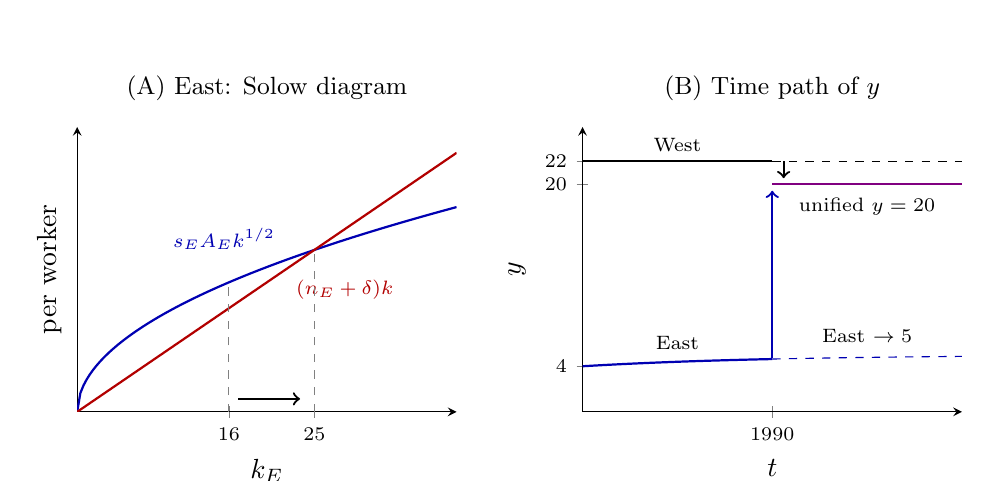
\begin{tikzpicture}
\begin{axis}[name=solow,width=6.4cm,height=5.2cm,axis lines=left,xmin=0,xmax=40,ymin=0,ymax=3.3,
  xlabel={$k_E$},ylabel={per worker},xtick={16,25},
  ytick=\empty,title={\small (A) East: Solow diagram},every tick label/.append style={font=\scriptsize}]
\addplot[domain=0:40,samples=120,thick,blue!70!black]{0.375*sqrt(x)} node[pos=0.55,above left,font=\scriptsize]{$s_EA_Ek^{1/2}$};
\addplot[domain=0:40,thick,red!70!black]{0.075*x} node[pos=0.55,below right,font=\scriptsize]{$(n_E+\delta)k$};
\draw[dashed,gray](axis cs:16,0)--(axis cs:16,1.5);
\draw[dashed,gray](axis cs:25,0)--(axis cs:25,1.875);
\draw[->,thick](axis cs:17,0.15)--(axis cs:23.5,0.15);
\end{axis}
\begin{axis}[at={(solow.east)},anchor=west,xshift=1.6cm,width=6.4cm,height=5.2cm,axis lines=left,
  xmin=-10,xmax=10,ymin=0,ymax=25,xlabel={$t$},ylabel={$y$},xtick={0},xticklabels={1990},
  ytick={4,20,22},title={\small (B) Time path of $y$},every tick label/.append style={font=\scriptsize}]
\addplot[thick,black]coordinates{(-10,22)(0,22)};
\addplot[dashed,black]coordinates{(0,22)(10,22)};
\addplot[domain=-10:0,samples=40,thick,blue!70!black]{5-exp(-0.1*(x+10))};
\addplot[domain=0:10,samples=40,dashed,blue!70!black]{5-exp(-0.1*(x+10))};
\addplot[thick,violet]coordinates{(0,20)(10,20)};
\draw[->,thick,blue!70!black](axis cs:0,4.7)--(axis cs:0,19.4);
\draw[->,thick,black](axis cs:0.6,22)--(axis cs:0.6,20.5);
\node[font=\scriptsize,anchor=south] at (axis cs:-5,22){West};
\node[font=\scriptsize,anchor=south] at (axis cs:-5,4.6){East};
\node[font=\scriptsize,anchor=south] at (axis cs:5,5.2){East $\to5$};
\node[font=\scriptsize,anchor=north] at (axis cs:5,19.6){unified $y=20$};
\end{axis}
\end{tikzpicture}\\
{\footnotesize Figure 1. (A) East starts below its own $k^*$. (B) Solid: actual paths; dashed: no-unification counterfactuals (schematic timing).}
\end{center}
\rubric{
\item Period-0 values: 1 pt. Steady-state formula and four numbers: 2 pts.
\item Direction for each region (West flat, East rising with falling growth): 1 pt.
\item Named \emph{conditional} convergence, gap in levels persists: 1 pt. Diagram with labelled curves, $k_0$, $k^*$: counts in this point if the words are missing.
\item Calling it ``divergence'' or ``absolute convergence'': max.\ 2 pts.
}
\end{sol}

\textbf{b)} (5 points) Unification: from 1990 all production uses West technology $A_W=2$ with the
pooled capital and labour of both regions. Compute the new $y$ and its change for West and for East
workers (in levels and in \% of the pre-unification value), and the change in aggregate German output
$Y$. Explain \emph{where} each region's gain or loss comes from.
\answerspace
\begin{sol}
\step{pooling}{$K=7744+256=8000$, $L=64+16=80\Rightarrow k_U=8000/80=100$, $y_U=2\sqrt{100}=\res{20}$.}
\step{per capita changes}{West: $22\to20$: $\res{-2,\ -9.09\%}$ (base 22). East: $4\to20$: $\res{+16,\ +400\%}$ (base 4).}
\step{West: source}{\textbf{Capital dilution}: same $A$, but $k$: $121\to100$ because East brings 20\% of the workers
and only 3.2\% of the capital. $K/L\downarrow\to y\downarrow$. Factor prices: $w=(1-\alpha)y$: $11\to10$ (West workers lose);
$r^K=\alpha y/k$: $1/11=0.091\to0.10$ (West capital owners gain).}
\step{East: source}{\textbf{Technology} $A:1\to2$ and \textbf{capital deepening} $k:16\to100$. Technology first:
$1\cdot4\to2\cdot4=8$ ($+4$), then capital $8\to20$ ($+12$). In logs (order-free):
$\ln5=\underbrace{\ln2}_{\text{technology}}+\underbrace{\tfrac12\ln(100/16)}_{\text{capital deepening}}=0.693+0.916$;
technology $\approx43\%$ of the log gain. $w_E$: $2\to10$.}
\step{aggregate}{Before: $Y=22\cdot64+4\cdot16=1408+64=1472$. After: $Y=20\cdot80=1600$.
$\Delta Y=\res{+128,\ +8.70\%}$. Germany-wide $y$: $1472/80=18.4\to20$. Source: East's $K$ and $L$ now work
with the better technology; West's loss per head is a \emph{redistribution} of capital, not lost output.}
\step{check}{$64\cdot(-2)+16\cdot(+16)=-128+256=128=\Delta Y$.}
\intuition{Per-capita and aggregate answers differ in sign for the West: West $y$ falls, yet German $Y$ rises.
``Not per capita for the West, but still an aggregate gain.''}
\refbib{Kurlat \S4.1--\S4.2, pp.~53--61; \S4.4, pp.~63--69 (factor prices).}
\rubric{
\item $k_U$, $y_U$ and the two per-capita changes with bases: 2 pts.
\item Sources: West = capital dilution (1 pt); East = technology + capital deepening (1 pt).
\item Aggregate $\Delta Y$ computed and interpreted: 1 pt.
\item Numbers with no source of gain/loss: max.\ 3 pts. Per capita only, no aggregate: max.\ 4 pts. Arithmetic slip: $-1$.
}
\end{sol}

\textbf{c)} (5 points) After unification Germany saves at the West's rate $s_W$ and its labour force
grows at the labour-weighted average of $n_W$ and $n_E$. Compute $k^*_U$ and $y^*_U$. Is unified
Germany below its steady state? Compare $y^*_U$ with $y^*_W$ and explain the difference.
\answerspace
\begin{sol}
\step{population growth}{$n_U=\dfrac{64\cdot0+16\cdot0.025}{80}=\dfrac{0.4}{80}=0.005$.}
\step{steady state}{$\dfrac{s_WA_W}{n_U+\delta}=\dfrac{0.55}{0.055}=10\Rightarrow\res{k^*_U=100,\ y^*_U=20}$.}
\step{position}{$k_U=100=k^*_U$: \res{\text{exactly at the steady state}} --- no transition; $y$ stays at 20,
$g_y=0$, and aggregate $Y$ grows at $n_U=0.5\%$.}
\step{comparison}{$y^*_U=20<y^*_W=22$ although $A$ and $s$ are the West's. The only difference is
$n_U=0.005>n_W=0$: break-even investment $(n+\delta)k$ is steeper ($0.055$ vs $0.05$), so each worker's capital
is diluted faster by newcomers and the same saving supports less $k$:
$n\uparrow\to(n+\delta)k\uparrow\to k^*\downarrow\to y^*\downarrow$.}
\intuition{Unification did not make the West's steady state unattainable because of the East's technology
(that was replaced) or its saving (not used): it is population growth alone. The 2-point gap is permanent,
unlike the 2-point loss in (b), which was a pure level redistribution.}
\refbib{Kurlat \S4.2, pp.~59--61; \S5.3, pp.~79--86 (convergence).}
\rubric{
\item $n_U$: 1 pt. $k^*_U$, $y^*_U$: 2 pts.
\item Position relative to SS: 1 pt. Explanation via $n$ and break-even investment: 1 pt.
\item Numbers with no explanation: max.\ 3 pts. Using unweighted $n$ ($0.0125$): $-1$ pt, rest graded on method.
}
\end{sol}
\begin{sol}
\gap{Lista 2, 1(b) (``divergence'' instead of conditional convergence); 1(c) (source of each region's gain/loss); 1(d) (numbers right, no explanation).}
\end{sol}

% =============================================================================
\block{III}{Microfoundations}{Lectures 4--6; Kurlat chs.~6, 7, 9 \,\textbullet\, 25 points}

\question{(10 points) Objective items.}

\textbf{a)} (3 points) A household has one unit of time, preferences $\ln c+\psi\ln l$ with $\psi=1$,
wage $w=10$, pays a tax $\tau$ on labour income and receives a lump-sum transfer $T=2$, so
$c=(1-\tau)w(1-l)+T$. The labour-income tax rises from $\tau=0.2$ to $\tau=0.5$ ($T$ unchanged). Hours:
\begin{options}
\item fall from 0.375 to 0.300: leisure became cheaper, an effect that would lower hours even with $T=0$.
\item stay at 0.500: with log utility the income and substitution effects cancel whatever $T$ is.
\item rise from 0.375 to 0.450: the lower net wage makes the household poorer, so it works more.
\item fall from 0.500 to 0.375: the tax lowers the price of leisure one-for-one with $\tau$.
\item fall from 0.375 to 0.300: the fixed $T$ grows relative to net earnings; with $T=0$ hours would not move.
\end{options}
\answer{E}
\begin{sol}
\step{labour supply}{MRS $=$ net wage: $\dfrac{\psi c}{l}=(1-\tau)w$ with $c=(1-\tau)w(1-l)+T$ $\Rightarrow$
$n=1-l=\dfrac{1}{1+\psi}-\dfrac{\psi T}{(1+\psi)(1-\tau)w}$. $\tau=0.2$: $0.5-\frac{2}{16}=0.375$; $\tau=0.5$: $0.5-\frac{2}{10}=0.300$.
With $T=0$, $n=0.5$ for any $\tau$: the effect runs only through $T$ (pure income effect), so A's reason is false.}
\refbib{Kurlat \S7.2, pp.~131--137.}
\gap{Lista 4, 1(b): the words described a substitution effect; the formula said the effect is through $T$.}
\end{sol}

\medskip
\textbf{b)} (3 points) In a search economy with $m(V,U)=\mu V^\alpha U^{1-\alpha}$, one firm posts one extra
vacancy. Which statement is correct?
\begin{options}
\item The posting firm and the other firms gain; unemployed workers lose, as matches per worker fall.
\item Unemployed workers gain ($f$ rises); other firms lose ($q$ falls); the posting firm gains privately.
\item The posting firm loses, because its own $q$ falls; this private cost is the congestion externality.
\item Everyone gains, since $m$ rises one-for-one with $V$, so the extra vacancy creates no externality.
\item Unemployed workers lose ($f$ falls); other firms gain ($q$ rises); the posting firm is unaffected.
\end{options}
\answer{B}
\begin{sol}
\step{signs}{$\theta=V/U\uparrow\Rightarrow f=\mu\theta^\alpha\uparrow$, $q=\mu\theta^{\alpha-1}\downarrow$; $\partial m/\partial V=\alpha q<q$
(not one-for-one: friction). The congestion cost lands on \emph{other} firms; the posting firm, which
expects profit, ignores both that cost and the benefit to workers.}
\refbib{Kurlat \S7.5, pp.~142--150.}
\gap{Lista 4, 2(d): externality placed on the posting firm itself.}
\end{sol}

\medskip
\textbf{c)} (2 points, T or F) A fall in matching efficiency $\mu$, which raises the vacancy rate
needed at every unemployment rate, is a movement along the Beveridge curve.
\answer{False}
\begin{sol}
\step{shift}{The Beveridge curve $s(1-u)=\mu v^\alpha u^{1-\alpha}$ (job destruction $=$ job creation) is drawn for a given
$\mu$. $\mu\downarrow$ moves every $(u,v)$ pair out: a \emph{shift}. A movement along it is a change in
tightness $\theta$ at given matching technology.}
\refbib{Kurlat \S7.1, pp.~127--131; \S7.5.}
\gap{Lista 4, 2(e): shift of vs movement along the Beveridge curve.}
\end{sol}

\medskip
\textbf{d)} (2 points, T or F) In the general-equilibrium economy with a fixed capital stock, no
investment, and preferences $\ln c+\psi\ln l$, a rise in TFP $A$ leaves hours worked unchanged.
\answer{True}
\begin{sol}
\step{equilibrium}{$\psi c/l=w$, $c=Y=AK^\alpha L^{1-\alpha}$, $w=(1-\alpha)AK^\alpha L^{-\alpha}$ $\Rightarrow$
$\psi\frac{L}{1-L}=1-\alpha\Rightarrow L=\frac{1-\alpha}{1-\alpha+\psi}$: no $A$. Equivalently
$\frac{d\ln L}{d\ln A}=\frac{1-\sigma}{\cdots}=0$ at $\sigma=1$: income and substitution effects cancel.}
\refbib{Kurlat \S9.1, pp.~165--168.}
\gap{Lista 5 (ungraded) and Lista 4, 1(b): with log utility, wage changes alone do not move hours.}
\end{sol}

% -----------------------------------------------------------------------------
\question{(15 points) A temporary tax cut financed by public debt. The Brazilian government
considers cutting this year's income tax and repaying the resulting debt next period. A household lives
two periods and solves
\[
\max_{c_1,c_2,a}\ u(c_1)+\beta u(c_2)\quad\text{s.t.}\quad c_1+a=y_1-\tau_1,\qquad c_2=y_2-\tau_2+(1+r)a,
\]
with $u(c)=\frac{c^{1-\sigma}}{1-\sigma}$ ($u=\ln c$ if $\sigma=1$), $\beta\in(0,1)$, $\sigma>0$. Baseline values:
$\sigma=1$, $\beta=0.8$, $r=0.25$ (a period is roughly a decade), $y_1=60$, $y_2=150$, $\tau_1=\tau_2=20$ (thousand reais).}

\textbf{a)} (5 points) By substituting the constraints into the objective (no Lagrangian needed), derive
the Euler equation and solve for $c_1$, $c_2$ and $a$ in closed form. Evaluate them at the baseline.
\answerspace
\begin{sol}
\step{substitute}{From period 1: $a=y_1-\tau_1-c_1$. Into period 2: $c_2=y_2-\tau_2+(1+r)(y_1-\tau_1-c_1)$.
Dividing by $1+r$: $c_1+\dfrac{c_2}{1+r}=\underbrace{y_1-\tau_1+\dfrac{y_2-\tau_2}{1+r}}_{\equiv\,W\ \text{(PV of after-tax income)}}$.}
\step{FOC}{$\max_{c_1}\ u(c_1)+\beta u\big(y_2-\tau_2+(1+r)(y_1-\tau_1-c_1)\big)$:\quad
$u'(c_1)-\beta(1+r)u'(c_2)=0\Rightarrow\res{c_1^{-\sigma}=\beta(1+r)\,c_2^{-\sigma}}$ (Euler: MRS $=1+r$).}
\step{solve}{$c_2=[\beta(1+r)]^{1/\sigma}c_1$. Into the PV constraint: $c_1\left[1+\beta^{1/\sigma}(1+r)^{\frac1\sigma-1}\right]=W$:
\[
\res{c_1=\frac{W}{D}},\quad \res{c_2=[\beta(1+r)]^{1/\sigma}\frac{W}{D}},\quad \res{a=y_1-\tau_1-\frac{W}{D}},\qquad
D\equiv1+\beta^{1/\sigma}(1+r)^{\frac1\sigma-1}.
\]}
\step{baseline}{$W=40+\frac{130}{1.25}=40+104=144$; $\sigma=1\Rightarrow D=1+\beta=1.8$.
$c_1=144/1.8=\res{80}$; $c_2=(0.8\cdot1.25)\cdot80=\res{80}$; $a=40-80=\res{-40}$ (borrows).}
\step{check}{$c_2=130+1.25\cdot(-40)=130-50=80$ \checkmark; Euler $1/80=0.8\cdot1.25/80$ \checkmark.}
\rubric{
\item Substitution and PV constraint: 1 pt. Euler equation: 1 pt.
\item Closed forms for $c_1,c_2$: 1 pt; \textbf{$a$ solved}: 1 pt. Baseline numbers: 1 pt.
\item Not solving for $a$: max.\ 4 pts. Lagrangian route is accepted. Arithmetic slip: $-1$.
}
\end{sol}

\textbf{b)} (5 points) Set $y_2=\tau_1=\tau_2=0$ (general $\sigma$). Compute $\partial c_1/\partial r$, isolate
the factor that determines its sign, and state, in words consistent with that sign, what happens to
$c_1$ when $r$ rises for $\sigma>1$, $\sigma=1$ and $\sigma<1$.
\answerspace
\begin{sol}
\step{set up}{$W=y_1$, so $c_1=\dfrac{y_1}{D(r)}$, $D(r)=1+\beta^{1/\sigma}(1+r)^{\frac{1-\sigma}{\sigma}}$.}
\step{differentiate}{$\dfrac{\partial D}{\partial r}=\beta^{1/\sigma}\,\dfrac{1-\sigma}{\sigma}\,(1+r)^{\frac{1-2\sigma}{\sigma}}$, so
\[
\frac{\partial c_1}{\partial r}=-\frac{y_1}{D^2}\frac{\partial D}{\partial r}
=\frac{y_1\,\beta^{1/\sigma}(1+r)^{\frac{1-2\sigma}{\sigma}}}{D^2}\cdot\underbrace{\frac{\sigma-1}{\sigma}}_{\text{determines the sign}}.
\]}
\step{sign}{$\res{\sigma>1:\ \partial c_1/\partial r>0}$;\quad $\res{\sigma=1:\ =0}$ ($c_1=y_1/(1+\beta)$);\quad $\res{\sigma<1:\ <0}$.}
\step{words}{The household is a pure saver. $r\uparrow$: \emph{substitution effect} --- $c_1$ is dearer in units of
$c_2$ $\to c_1\downarrow$; \emph{income effect} --- a saver is richer $\to c_1\uparrow$. $\sigma$ is the curvature of $u$;
$1/\sigma$ is the elasticity of intertemporal substitution. $\sigma>1$ (low EIS): income effect dominates,
so $c_1$ \textbf{rises} and saving falls. $\sigma<1$: substitution dominates, $c_1$ \textbf{falls}. $\sigma=1$: they cancel.}
\refbib{Kurlat \S6.2, pp.~112--115.}
\rubric{
\item $c_1(r)$ and correct derivative: 2 pts. Sign factor isolated: 1 pt.
\item Words matching the sign for each case (income vs substitution, saver): 2 pts.
\item Correct sign condition but words with the opposite direction (e.g.\ ``$\sigma>1$, $c_1$ falls''): max.\ 2 pts.
}
\end{sol}

\textbf{c)} (5 points) Return to the baseline. The government cuts $\tau_1$ by $\Delta=10$ and raises
$\tau_2$ by $(1+r)\Delta$. (i) Find the effect on $c_1$, $c_2$ and $a$. Does the timing of taxes matter?
(ii) Now the household faces a borrowing limit $a\ge-b$ with $b=20$. Find $c_1$, $c_2$, $a$ before and
after the same tax change. (iii) Give two concrete examples of Brazilian households for whom such a
limit is likely to bind.
\answerspace
\begin{sol}
\step{(i) PV of taxes}{$\tau_1'+\dfrac{\tau_2'}{1+r}=(\tau_1-\Delta)+\dfrac{\tau_2+(1+r)\Delta}{1+r}=\tau_1+\dfrac{\tau_2}{1+r}=36$:
$W$ unchanged $\Rightarrow$ $\res{\Delta c_1=\Delta c_2=0,\ \Delta a=+\Delta=+10}$.
Numbers: $\tau_1=10$, $\tau_2=20+12.5=32.5$; $W=50+117.5/1.25=50+94=144$; $c_1=c_2=80$; $a=50-80=-30$.
The household saves the whole cut to pay the future tax (Ricardian equivalence): \textbf{timing does not
matter}, only the PV of taxes.}
\step{(ii) before}{Desired $a=-40<-20$ $\Rightarrow$ limit binds: $a=-20$, $c_1=y_1-\tau_1+b=40+20=\res{60}$,
$c_2=130+1.25(-20)=130-25=\res{105}$. Euler becomes an inequality: $u'(c_1)=1/60>\beta(1+r)u'(c_2)=1/105$.}
\step{(ii) after}{Desired $a=-30<-20$: still binds. $a=-20$; $c_1=50+20=\res{70}$ ($+10=\Delta$);
$c_2=117.5-25=\res{92.5}$ ($-12.5=-(1+r)\Delta$). MPC out of the cut $=1$; timing \textbf{matters}.
(It keeps binding while $-40+\Delta<-20$, i.e.\ $\Delta<20$.)}
\step{(iii) examples}{(1) A young medical resident or university student with low income now and high
expected income later, and no collateral. (2) An informal worker (or someone with a negative record at
Serasa) whose income fell temporarily and who cannot borrow against future earnings.}
\begin{center}
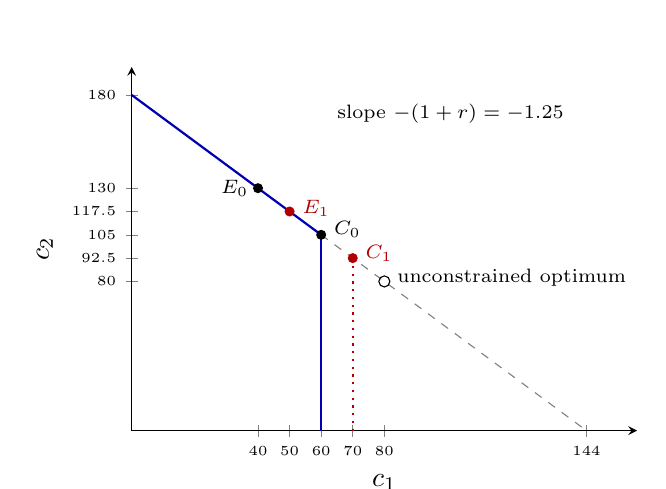
\begin{tikzpicture}
\begin{axis}[width=8cm,height=6.2cm,axis lines=left,xmin=0,xmax=160,ymin=0,ymax=195,
  xlabel={$c_1$},ylabel={$c_2$},xtick={40,50,60,70,80,144},ytick={80,92.5,105,117.5,130,180},
  every tick label/.append style={font=\tiny}]
\addplot[domain=60:144,dashed,gray]{1.25*(144-x)};
\addplot[domain=0:60,thick,blue!70!black]{1.25*(144-x)};
\draw[thick,blue!70!black](axis cs:60,105)--(axis cs:60,0);
\draw[dotted,thick,red!70!black](axis cs:70,92.5)--(axis cs:70,0);
\addplot[only marks,mark=*,mark size=1.6pt]coordinates{(40,130)(60,105)};
\addplot[only marks,mark=*,mark size=1.6pt,red!70!black]coordinates{(50,117.5)(70,92.5)};
\addplot[only marks,mark=o,mark size=2pt]coordinates{(80,80)};
\node[font=\scriptsize,anchor=east] at (axis cs:40,130){$E_0$};
\node[font=\scriptsize,anchor=west,red!70!black] at (axis cs:51,119){$E_1$};
\node[font=\scriptsize,anchor=west] at (axis cs:61,108){$C_0$};
\node[font=\scriptsize,anchor=west,red!70!black] at (axis cs:71,95){$C_1$};
\node[font=\scriptsize,anchor=west] at (axis cs:81,82){unconstrained optimum};
\node[font=\scriptsize,anchor=west] at (axis cs:62,170){slope $-(1+r)=-1.25$};
\end{axis}
\end{tikzpicture}\\
{\footnotesize Figure 2. The budget line is the same before and after the swap ($W=144$); the endowment slides
from $E_0$ to $E_1$ along it. The limit $c_1\le y_1-\tau_1+b$ moves from 60 to 70, so the constrained choice moves
from $C_0$ to $C_1$.}
\end{center}
\intuition{Ricardian equivalence needs the household to be able to move resources across periods at $r$.
When the limit binds, the tax cut is the loan the market would not give, and it is consumed one-for-one.}
\refbib{Kurlat \S6.2--\S6.4, pp.~120--126.}
\rubric{
\item (i) PV argument and $\Delta c_1=\Delta c_2=0$, $\Delta a=\Delta$: 2 pts.
\item (ii) Binding check and $c_1$ before/after: 1.5 pts (diagram with kink, labelled axes and points counts here).
\item (iii) Two examples: 1.5 pts (0.75 each).
\item Proving PV-only and then stating ``timing matters'' in the unconstrained case: max.\ 2 pts. One example only: $-0.75$.
}
\end{sol}
\begin{sol}
\gap{Lista 3, 1(a)(d) (never solved for $a$); 1(c) (right sign condition, opposite words); 1(e) (PV proved, then ``timing matters''); 2(b) (one example where two were asked).}
\end{sol}

% =============================================================================
\block{IV}{Money, inflation and AD--AS}{Lectures 7--9; Kurlat chs.~10--11; Benigno (2015) \,\textbullet\, 25 points}

\question{(10 points) Objective items.}

\textbf{a)} (3 points) About the quantity equation $MV=PY$:
\begin{options}
\item It is a theory of money demand: with $Y$ fixed, doubling $M$ doubles $P$ at every horizon.
\item It is an identity which proves neutrality, because $V$ and $Y$ are constant by definition.
\item It is a behavioural equation: $V$ is a structural parameter that the central bank sets.
\item It is an identity, since $V\equiv PY/M$; causation needs assumptions on $V$ and on what is exogenous.
\item It is an identity which proves causation runs from $P$ to $M$, because firms set prices first.
\end{options}
\answer{D}
\begin{sol}
\step{residual}{$V$ is measured as $PY/M$, so the equation holds for any data. It becomes a theory only with
an assumption on $V$ (e.g.\ stable, or given by a money-demand model) and on which variable is exogenous.}
\refbib{Kurlat \S10.4, pp.~199--204; \S11.2.}
\gap{Lista 6, 1(a): $V$ as a residual; causation needs an assumption.}
\end{sol}

\medskip
\textbf{b)} (3 points) In steady state with constant $i$, $\pi=\mu-\eta g$. The central bank targets $\pi^*=3\%$
with $g=2\%$ and sets $\mu$ assuming $\eta=1$ (Cambridge). Money demand is actually Baumol--Tobin. Inflation is:
\begin{options}
\item $2\%$
\item $3\%$
\item $4\%$
\item $5\%$
\item $6\%$
\end{options}
\answer{C}
\begin{sol}
\step{compute}{Chosen $\mu=\pi^*+1\cdot g=5\%$. Baumol--Tobin: $\eta=\tfrac12$, so $\pi=5\%-\tfrac12\cdot2\%=\res{4\%}$.
Desired real balances grow at $1\%$, not $2\%$: the extra money goes into prices.}
\refbib{Kurlat \S11.2, pp.~205--215.}
\gap{Lista 6, 2(b): inflation-targeting error formula.}
\end{sol}

\medskip
\textbf{c)} (2 points, T or F) When the central bank targets the nominal interest rate, the money-market
equilibrium $M=p\,m^D(Y,i)$ determines the quantity of money.
\answer{True}
\begin{sol}
\step{endogenous $M$}{With $i$ fixed by policy, and $p$, $Y$ given, $M$ must supply whatever $p\,m^D(Y,i)$ demands: the
central bank accommodates by open-market operations. Under a money target it is the reverse: $M$ given, $i$ adjusts.}
\refbib{Kurlat \S11.1--\S11.2; Benigno \S3 (policy sets $i$).}
\gap{Lista 6, 1(d): under an interest-rate target the money market determines $M$.}
\end{sol}

\medskip
\textbf{d)} (2 points, T or F) In Benigno's AD--AS model, a temporary rise in firms' desired mark-up
shifts the AD curve to the left.
\answer{False}
\begin{sol}
\step{which curve}{The mark-up enters the price-setting (AS) block: natural output falls, AS shifts up/left. AD comes
from the Euler equation and the policy rule, where $\mu$ does not appear: AD does not move (stagflation along AD).}
\refbib{Benigno (2015) \S4 and \S7.}
\gap{Shift of vs movement along AD/AS (taxonomy).}
\end{sol}

% -----------------------------------------------------------------------------
\question{(15 points) Pix and the demand for money. Since 2020 Pix, Brazil's instant-payment
system, has lowered the cost of turning deposits into means of payment. Model real money demand with
Baumol--Tobin, $m^D=\sqrt{\dfrac{FY}{2i}}$, where $F$ is the real cost of each conversion. Assume real
output grows at $g=2\%$, $F$ falls at the constant rate $\dot F/F=f=-4\%$, and $i$ is constant. The
money market clears: $M=p\,m^D(Y,i,F)$.}

\textbf{a)} (5 points) Derive velocity $V$ implied by this model. Explain why $V$ is not constant, and
compute its growth rate under the assumptions above. Interpret velocity in words.
\answerspace
\begin{sol}
\step{definition}{$V\equiv\dfrac{pY}{M}=\dfrac{pY}{p\,m^D}=\dfrac{Y}{\sqrt{FY/2i}}=\res{\sqrt{\dfrac{2iY}{F}}}$.}
\step{not constant}{$V$ depends on $i$ (opportunity cost of holding money $\uparrow\Rightarrow V\uparrow$), on $Y$
(economies of scale in cash management, $\partial\ln V/\partial\ln Y=\tfrac12$) and on $F$ (payment technology,
$\partial\ln V/\partial\ln F=-\tfrac12$).}
\step{growth}{$\dfrac{\dot V}{V}=\tfrac12\dfrac{\dot i}{i}+\tfrac12 g-\tfrac12 f=0+1\%+2\%=\res{3\%\ \text{per year}}$.}
\step{interpret}{$V$ is the number of times the average real balance is spent per period. In $MV=PY$ it
is a residual; Baumol--Tobin gives it a theory: cheaper conversions $\to$ smaller average balances per real
transaction $\to$ each real balance turns over faster.}
\refbib{Kurlat \S10.4, pp.~199--204.}
\rubric{
\item $V=\sqrt{2iY/F}$ derived: 2 pts.
\item Dependence on $i$, $Y$, $F$ with signs: 1 pt. Growth $3\%$: 1 pt. Interpretation: 1 pt.
\item Treating $V$ as constant or exogenous: max.\ 2 pts.
}
\end{sol}

\textbf{b)} (5 points) By totally differentiating $M=p\,m^D(Y,i,F)$ with respect to time, show that in
steady state $\pi=\mu-\tfrac12(g+f)$. Before Pix ($f=0$) the BCB grew money at the rate that delivered
$\pi=3\%$. Which money growth $\mu$ delivers $3\%$ after Pix? What inflation results if the BCB keeps the
old $\mu$? Explain the mechanism in words.
\answerspace
\begin{sol}
\step{differentiate}{$\dot M=\dot p\,m^D+p\left[\dfrac{\partial m^D}{\partial Y}\dot Y+\underbrace{\dfrac{\partial m^D}{\partial i}\dot i}_{=0\ (i\ \text{const.})}+\dfrac{\partial m^D}{\partial F}\dot F\right]$.}
\step{divide by $M=p\,m^D$}{$\mu=\pi+\underbrace{\dfrac{\partial m^D}{\partial Y}\dfrac{Y}{m^D}}_{\eta_Y}g+\underbrace{\dfrac{\partial m^D}{\partial F}\dfrac{F}{m^D}}_{\eta_F}f$.
From $m^D=(FY/2i)^{1/2}$: $\eta_Y=\eta_F=\tfrac12$ $\Rightarrow$ $\res{\pi=\mu-\tfrac12(g+f)}$.}
\step{before Pix}{$f=0$: $\mu=\pi^*+\tfrac12g=3\%+1\%=4\%$.}
\step{after Pix}{$\mu=\pi^*+\tfrac12(g+f)=3\%+\tfrac12(2\%-4\%)=3\%-1\%=\res{2\%}$.
Keeping $\mu=4\%$: $\pi=4\%-\tfrac12(-2\%)=\res{5\%}$.}
\step{mechanism}{$F\downarrow\to$ households hold smaller real balances $\to$ desired real money grows at
$\tfrac12(g+f)=-1\%$ instead of $+1\%$ $\to$ the same $\mu=4\%$ chases a \emph{shrinking} demand for real balances
$\to$ excess money $\to p$ grows faster: $\pi=5\%$. Equivalently, velocity rises at $3\%$. It is lower money
\emph{demand}, not ``cheap money''.}
\refbib{Kurlat \S11.2, pp.~205--215.}
\rubric{
\item Total differentiation with $\dot i=0$ struck: 1 pt. Elasticities named and $=\tfrac12$: 1 pt.
\item $\mu=2\%$ and $\pi=5\%$: 2 pts (1 each). Mechanism via money demand/velocity: 1 pt.
\item Explaining the effect as ``cheaper money'' or ``more money supply'': max.\ 3 pts. Arithmetic slip: $-1$.
}
\end{sol}

\textbf{c)} (5 points) Suppose instead the BCB sets the Selic (an interest-rate target $i^*$) and lets the
money supply be whatever it must be. When Pix lowers $F$, what adjusts in the money market in the short
run (prices sticky)? Is the Pix effect inflationary under this regime in the long run? Contrast with the
money-growth rule of (b).
\answerspace
\begin{sol}
\step{short run}{$F\downarrow\Rightarrow m^D\downarrow$ at every $i$ (curve shifts left). If $M$ stayed put, excess money
would push $i$ below $i^*$. To hold $i=i^*$ the BCB drains money (sells bonds):
$F\downarrow\to m^D\downarrow\to$ BCB sells bonds $\to M\downarrow$, $i=i^*$ unchanged $\to$ AD unchanged $\to y,p$ unchanged.
\res{\text{$M$ adjusts; $i$ does not.}}}
\step{long run}{$\pi$ is pinned by the target: $\pi=3\%$. Money growth becomes endogenous:
$\mu=\pi+\tfrac12(g+f)=3\%+\tfrac12(2\%-4\%)=\res{2\%}$. \res{\text{Not inflationary}}; Pix shows up only as slower
growth of money aggregates and rising velocity.}
\step{contrast}{Under a money-growth rule ($\mu=4\%$ fixed) the same shock raises $\pi$ to $5\%$, as in (b). The regime
decides whether a money-demand shock reaches prices: with an $i$ target the central bank absorbs it.}
\begin{center}
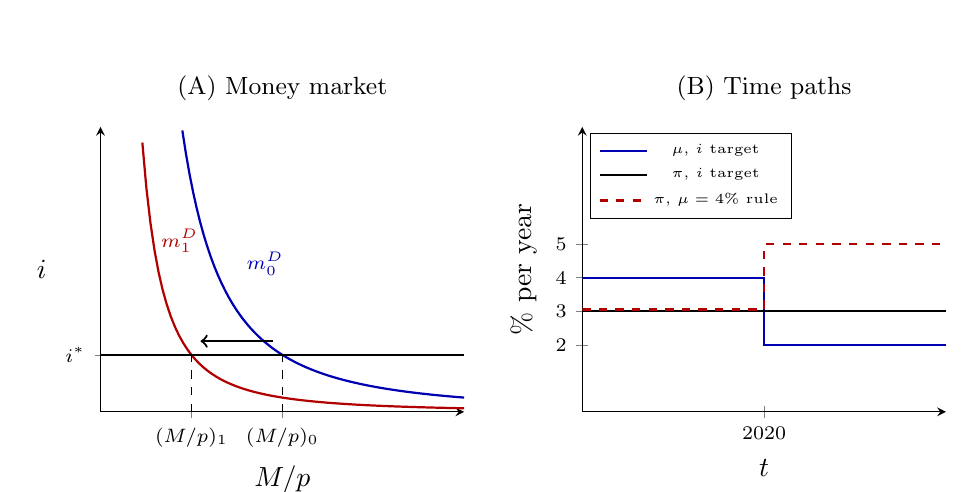
\begin{tikzpicture}
\begin{axis}[name=mm,width=6.2cm,height=5.2cm,axis lines=left,xmin=0,xmax=4,ymin=0,ymax=2.5,
  xlabel={$M/p$},ylabel={$i$},xtick={1,2},xticklabels={$(M/p)_1$,$(M/p)_0$},ylabel style={rotate=-90},ytick={0.5},yticklabels={$i^*$},
  title={\small (A) Money market},every tick label/.append style={font=\scriptsize}]
\addplot[domain=0.9:4,samples=80,thick,blue!70!black]{2/x^2};
\node[font=\scriptsize,blue!70!black,anchor=west] at (axis cs:1.5,1.3){$m^D_0$};
\addplot[domain=0.46:4,samples=80,thick,red!70!black]{0.5/x^2};
\node[font=\scriptsize,red!70!black] at (axis cs:0.87,1.5){$m^D_1$};
\addplot[thick,black]coordinates{(0,0.5)(4,0.5)};
\draw[dashed](axis cs:2,0)--(axis cs:2,0.5);
\draw[dashed](axis cs:1,0)--(axis cs:1,0.5);
\draw[->,thick](axis cs:1.9,0.62)--(axis cs:1.1,0.62);
\end{axis}
\begin{axis}[at={(mm.east)},anchor=west,xshift=1.5cm,width=6.2cm,height=5.2cm,axis lines=left,
  xmin=-5,xmax=5,ymin=0,ymax=8.5,xlabel={$t$},ylabel={\% per year},xtick={0},xticklabels={2020},
  ytick={2,3,4,5},title={\small (B) Time paths},every tick label/.append style={font=\scriptsize},
  legend style={font=\tiny,at={(0.02,0.98)},anchor=north west}]
\addplot[thick,blue!70!black]coordinates{(-5,4)(0,4)(0,2)(5,2)};
\addlegendentry{$\mu$, $i$ target}
\addplot[thick,black]coordinates{(-5,3)(5,3)};
\addlegendentry{$\pi$, $i$ target}
\addplot[dashed,thick,red!70!black]coordinates{(-5,3.05)(0,3.05)(0,5)(5,5)};
\addlegendentry{$\pi$, $\mu=4\%$ rule}
\end{axis}
\end{tikzpicture}\\
{\footnotesize Figure 3. (A) Lower $F$ shifts money demand left from $m^D_0=m^D(F_0)$ to $m^D_1=m^D(F_1)$ (drawn for $F_1=F_0/4$, which halves $m^D$); at $i^*$ real balances fall from $(M/p)_0$ to $(M/p)_1$.
(B) Under the $i$ target $\mu$ falls from 4\% to 2\% and $\pi$ stays at 3\%; under a fixed $\mu=4\%$, $\pi$ rises to 5\%.}
\end{center}
\intuition{Money is endogenous under an interest-rate rule: the central bank supplies the money people want at $i^*$.
A payment innovation that lowers money demand therefore changes $M$, not $i$, and leaves AD and inflation alone.}
\refbib{Kurlat \S11.1--\S11.2, pp.~205--215; Benigno (2015) \S3 (the central bank sets $i$).}
\rubric{
\item Short run: $m^D$ shifts left, $M$ adjusts, $i$ unchanged, no AD effect: 2 pts (arrow chain or diagram with labelled axes, curves and shift direction).
\item Long run: $\pi$ anchored, $\mu$ endogenous $=2\%$: 2 pts. Contrast with the money rule: 1 pt.
\item Stating that the BCB keeps $M$ fixed (or that $i$ falls) under an $i$ target: max.\ 2 pts.
}
\end{sol}
\begin{sol}
\gap{Lista 6, 1(a)(b) ($V$ a residual, velocity interpreted); 1(c) (mechanism; flexible-price neutrality: in the long run only $\pi$ and nominal aggregates move); 1(d) ($M$ endogenous under an $i$ target); 2(c) (falling $F$ = lower money demand, not ``cheap money'').}
\end{sol}

\end{document}
"
% Check fonts afterwards: pdffonts simulado-01-solutions.pdf  (all Type 1)
% Every number in the key is verified by simulado_codigo/check_simulado_01.py
% =============================================================================
\documentclass[11pt,a4paper]{article}
\usepackage[utf8]{inputenc}
\usepackage[T1]{fontenc}
\usepackage{lmodern}   % Type 1 vector fonts (replaces PK bitmaps)
\usepackage{cmap}      % ToUnicode CMap -> copyable text
\usepackage[english]{babel}
\usepackage{amsmath,amssymb,amsfonts}
\usepackage[a4paper,margin=2.2cm]{geometry}
\usepackage{enumitem}
\usepackage{fancyhdr}
\usepackage{comment}
\def\CommentCutFile{simulado-01.cut} % private cut file: sibling sources build in this folder
\usepackage{xcolor}
\usepackage{booktabs}
\usepackage{microtype}
\usepackage{pgfplots}
\pgfplotsset{compat=1.16}

% ====================== CONFIGURATION ======================
\newif\ifsolucoes
\ifdefined\withsolutions\solucoestrue\else\solucoesfalse\fi

\newcommand{\course}{Macroeconomics I --- MPE Insper}
\newcommand{\examtitle}{Mock Final Exam 1 (Simulado 1)}
\newcommand{\answerheight}{5.2cm}

% ====================== MACHINERY ======================
\ifsolucoes\includecomment{sol}\else\excludecomment{sol}\fi

\pagestyle{fancy}\fancyhf{}
\lhead{\footnotesize\course}
\rhead{\footnotesize\examtitle\ifsolucoes{} --- Solutions and Rubric\fi}
\cfoot{\footnotesize\thepage}
\renewcommand{\headrulewidth}{0.3pt}
\setlength{\headheight}{14pt}

\setlist{topsep=2pt,itemsep=2pt}
\newcounter{questao}

\newcommand{\block}[3]{\bigskip\noindent
  {\large\bfseries\color{blue!55!black}Block #1 --- #2}\par\noindent{\small\textit{(#3)}}\par
  \noindent\rule{\linewidth}{0.3pt}\smallskip}
\newcommand{\question}[1]{\refstepcounter{questao}\medskip\noindent
  \textbf{Question \thequestao.}~#1\par}
\newenvironment{options}{\begin{enumerate}[label=\Alph*.,leftmargin=2.2em,topsep=1pt]}{\end{enumerate}}
\newcommand{\answer}[1]{\ifsolucoes\par\noindent\textbf{Answer:}~#1\fi}
\newcommand{\answerspace}{\ifsolucoes\else\par\textit{Solution:}\vspace{\answerheight}\par\fi}
\newcommand{\step}[2]{\par\smallskip\noindent\textbf{Step --- #1.}~#2}
\newcommand{\intuition}[1]{\par\smallskip\noindent\textit{Intuition.}~#1}
\newcommand{\refbib}[1]{\par\smallskip\noindent{\footnotesize\color{black!60}\textbf{Ref:} #1}}
\newcommand{\gap}[1]{\par\smallskip\noindent{\footnotesize\color{red!55!black}\textbf{Gap targeted:} #1}}
\newcommand{\rubric}[1]{\par\smallskip\noindent\textbf{Rubric.}\begin{itemize}[leftmargin=1.4em,topsep=1pt]#1\end{itemize}}
\newcommand{\res}[1]{\boxed{#1}}

% =============================================================================
\begin{document}
\begin{center}
  {\Large\bfseries \course}\\[2pt]
  {\large \examtitle}\ifsolucoes\\[2pt]\textit{Solutions and Grading Rubric}\fi
\end{center}
\vspace{2pt}

{\footnotesize\noindent\textbf{Instructions.} Four blocks of 25 points each (100 points).
Suggested time: 3 hours. Multiple-choice items: mark the single correct option (no penalty
for wrong answers). \emph{True/False} items: every 2 wrong items cancel 1 right item
(score $=\max\{0,\ \text{right}-\text{wrong}/2\}\times$ item value); blank items do not
count as wrong. Discursive questions: show every step; box your final answers. Numerical
values are illustrative. Notation follows Kurlat (2020).\par}

% =============================================================================
\block{I}{Measurement}{Lecture 1; Kurlat chs.~1--2 \,\textbullet\, 25 points}

\question{(10 points) Objective items.}

\textbf{a)} (3 points) An economy produces two goods. In Year~1, good $X$ costs 10 and
$10$ units are produced; good $Z$ costs 5 and $20$ units are produced. In Year~2, $X$ costs 5
and $20$ units are produced; $Z$ costs 10 and $16$ units are produced. Real GDP growth from
Year~1 to Year~2 measured at Year-1 prices and at Year-2 prices is, respectively:
\begin{options}
\item $40\%$ at Year-1 prices; $4\%$ at Year-2 prices.
\item $4\%$ at Year-1 prices; $40\%$ at Year-2 prices.
\item $30\%$ at Year-1 prices; $30\%$ at Year-2 prices.
\item $40\%$ at Year-1 prices; $30\%$ at Year-2 prices.
\item $20.7\%$ at Year-1 prices; $20.7\%$ at Year-2 prices.
\end{options}
\answer{A}
\begin{sol}
\step{compute}{Nominal: $Y_1=10\cdot10+5\cdot20=200$, $Y_2=5\cdot20+10\cdot16=260$.
Year-2 output at Year-1 prices: $10\cdot20+5\cdot16=280\Rightarrow 280/200-1=\res{40\%}$.
Year-1 output at Year-2 prices: $5\cdot10+10\cdot20=250\Rightarrow 260/250-1=\res{4\%}$.
C is nominal growth ($260/200-1$), E is the Fisher index ($\sqrt{1.40\cdot1.04}-1$), B swaps the bases.}
\refbib{Kurlat \S1.2, pp.~22--25.}
\gap{Lista 1, 1(b)(c): Laspeyres/Paasche arithmetic slips.}
\end{sol}

\medskip
\textbf{b)} (3 points) Why is the GDP of a low-income country, converted into dollars at the
market exchange rate, systematically \emph{lower} than the same GDP converted at purchasing
power parity (PPP)?
\begin{options}
\item Tariffs and transport costs keep traded-goods prices apart across countries, and the market rate cannot close that gap.
\item Non-traded goods and services are cheap where wages are low, and the market rate, set by traded goods, ignores this.
\item The market rate is driven by capital flows rather than by trade, so it undervalues every poor-country currency by the same factor.
\item Large informal sectors are left out of the official statistics, so a big share of production is missing from measured GDP.
\item Quotas and import licences raise traded-goods prices in poor countries, which inflates their measured price level.
\end{options}
\answer{B}
\begin{sol}
\step{mechanism}{The market rate equalises (roughly) the prices of \emph{traded} goods. Non-traded
output (housing, haircuts, public services) is priced off local wages, which are low where
productivity in tradables is low (Balassa--Samuelson). Converting at the market rate values that
output at rich-country prices nobody there pays $\Rightarrow$ understates real output. A and E are
frictions in traded goods (and E goes the wrong way); D lowers GDP at \emph{any} conversion rate, so it
cannot explain the gap between the two; C has no mechanism.}
\refbib{Kurlat \S1.2, pp.~25--27.}
\gap{Lista 1, 1(e): PPP gap explained with trade costs instead of non-tradables.}
\end{sol}

\medskip
\textbf{c)} (2 points, T or F) In a two-good economy, if between two years quantities shift
toward the good whose relative price fell, then real GDP growth measured at initial-year prices
exceeds real GDP growth measured at final-year prices.
\answer{True}
\begin{sol}
\step{proof}{With goods $x,z$: $\sum p^0q^1\cdot\sum p^1q^0-\sum p^0q^0\cdot\sum p^1q^1
=(q^1_xq^0_z-q^0_xq^1_z)(p^0_xp^1_z-p^0_zp^1_x)$. The first factor is $>0$ iff quantities moved toward
$x$; the second is $>0$ iff the relative price of $x$ fell. Both hold $\Rightarrow$ Laspeyres growth $>$
Paasche growth (substitution bias). Item (a) is an instance: 40\% $>$ 4\%.}
\refbib{Kurlat \S1.2, pp.~22--25.}
\gap{Lista 1, 1(c): direction of the substitution bias not explained.}
\end{sol}

\medskip
\textbf{d)} (2 points, T or F) Brazil imports all the smartphones it consumes and produces none.
A rise in their dollar price raises the IPCA and the GDP deflator by the same proportion, since both
measure ``the price level''.
\answer{False}
\begin{sol}
\step{coverage}{The GDP deflator $=P Y^{\text{nominal}}/Y^{\text{real}}$ covers only goods
\emph{produced} in Brazil; imports are subtracted in $Y=C+I+G+X-M$. The IPCA prices a consumer basket,
imported goods included. So the IPCA rises and the deflator does not move.}
\refbib{Kurlat \S1.2, pp.~22--25.}
\gap{Deflator vs CPI (taxonomy of \texttt{rules/00\_estilo\_avaliacao.md}); reciprocal trap.}
\end{sol}

% -----------------------------------------------------------------------------
\question{(15 points) IBGE and the smartphone boom. Consider a stylised Brazil producing only
soybeans ($s$) and smartphones ($m$). Values in billions of reais; population in millions.}

\begin{center}
\begin{tabular}{lcccc c}
\toprule
 & $p_s$ & $q_s$ & $p_m$ & $q_m$ & Population \\
\midrule
2015 & 10 & 60 & 20 & 20 & 200 \\
2025 & 12 & 60 & 12 & 40 & 210 \\
\bottomrule
\end{tabular}
\end{center}

\textbf{a)} (5 points) Compute nominal GDP in both years; real GDP in 2015 prices and in 2025
prices; the real growth rate between 2015 and 2025 in each base; and the Fisher (chained) growth
rate. State which year's value is in the denominator of each rate.
\answerspace
\begin{sol}
\step{nominal}{$PY_{2015}=10\cdot60+20\cdot20=600+400=\res{1000}$;\;
$PY_{2025}=12\cdot60+12\cdot40=720+480=\res{1200}$. Nominal growth $1200/1000-1=20\%$.}
\step{base 2015 (Laspeyres)}{$Y_{2025}^{(2015)}=10\cdot60+20\cdot40=600+800=1400$;\;
$Y_{2015}^{(2015)}=1000$.\; $g=\dfrac{1400}{1000}-1=\res{40\%}$ (2015 value in the denominator).}
\step{base 2025 (Paasche)}{$Y_{2015}^{(2025)}=12\cdot60+12\cdot20=720+240=960$;\;
$Y_{2025}^{(2025)}=1200$.\; $g=\dfrac{1200}{960}-1=0.25=\res{25\%}$ (2015 value, at 2025 prices, in the denominator).}
\step{Fisher}{$1+g_F=\sqrt{1.40\times1.25}=\sqrt{1.75}=1.3229\Rightarrow\res{g_F=32.29\%}$. With two years
the chain has one link, so chained $=$ Fisher.}
\step{check}{$25\%<32.29\%<40\%$: the geometric mean lies between the two bases.
Implied deflator: $1200/1400=0.857$ (base 2015).}
\rubric{
\item Nominal GDP, both years: 1 pt.
\item Real GDP in both bases and the two growth rates: 2 pts (1 each).
\item Fisher: 1 pt. Denominators stated: 1 pt.
\item Arithmetic slip with correct method: $-1$ pt (once). Swapping the bases (40\% at 2025 prices): max.\ 2 pts.
}
\end{sol}

\textbf{b)} (5 points) The two bases give different answers. For each one, say whether it
overstates or understates growth relative to the Fisher index, and explain \emph{why}, using the
movement of relative prices and quantities in the table.
\answerspace
\begin{sol}
\step{what moved}{Relative price $p_m/p_s$: $20/10=2\ \to\ 12/12=1$ (smartphones got \emph{cheaper}).
Quantities: $q_s$ constant, $q_m$: $20\to40$. Quantities moved \emph{toward} the good whose relative price fell.}
\step{2015 prices}{The 20 extra smartphones are valued at the \emph{old, high} price 20: the gain is $20\cdot20=400$
on a base of 1000 $\Rightarrow$ 40\% $\Rightarrow$ \res{\text{overstates}}.}
\step{2025 prices}{The same 20 phones are valued at the \emph{new, low} price 12: gain $12\cdot20=240$ on 960
$\Rightarrow$ 25\% $\Rightarrow$ \res{\text{understates}}.}
\step{name}{Arrow chain: $p_m/p_s\downarrow\ \to\ q_m/q_s\uparrow$ (substitution) $\to$ fast-growing good weighted
at its high old price (Laspeyres $\uparrow$) or at its low new price (Paasche $\downarrow$). This is
\textbf{substitution bias}; statistical agencies (IBGE included) chain the index with
previous-year prices to shrink it.}
\intuition{Both numbers are correct arithmetic; they answer ``how much more output, valued at which prices?''.
An observer who sees only one base would wrongly attribute the difference to real performance. The bias is
not a convention: its sign is fixed by the negative co-movement of prices and quantities.}
\refbib{Kurlat \S1.2, pp.~22--25.}
\rubric{
\item Relative price and quantity movements identified: 1 pt.
\item Direction of each bias: 2 pts (1 each).
\item Cause (valuing the fast-growing good at high vs low price; substitution bias named): 2 pts.
\item ``The base year is a convention'' with no direction or cause: max.\ 1 pt.
}
\end{sol}

\textbf{c)} (5 points) Compute real GDP growth per capita in each base and with Fisher. Which
number, aggregate or per capita, answers ``did the average Brazilian become better off?''
and which answers ``how much bigger is the Brazilian economy?'' What does neither answer?
\answerspace
\begin{sol}
\step{population}{$n=210/200-1=5\%$. Per capita: $1+g_y=\dfrac{1+g_Y}{1+n}$.}
\step{per capita}{2015 prices: $1.40/1.05-1=\res{33.33\%}$; 2025 prices: $1.25/1.05-1=\res{19.05\%}$;
Fisher: $1.3229/1.05-1=\res{25.99\%}$.}
\step{levels}{Per capita 2015: $1000/200=5$ thousand reais; 2025 at 2015 prices: $1400/210=6.67$.}
\step{interpret}{Aggregate ($32.29\%$ Fisher): size of the economy, tax base, market size.
Per capita ($25.99\%$): average living standard $\Rightarrow$ the welfare question. Neither measures
consumption vs.\ investment, leisure, distribution or non-market output (Kurlat ch.~2: GDP per
capita is a proxy for welfare, not welfare).}
\rubric{
\item Correct formula $(1+g_Y)/(1+n)$: 1 pt; three per-capita rates: 2 pts.
\item Aggregate vs per capita matched to the two questions: 1 pt. Limits of GDP per capita: 1 pt.
\item Answering only per capita (or only aggregate): max.\ 2 pts. Subtracting $n$ instead of dividing: $-1$ pt only if stated as exact.
}
\end{sol}
\begin{sol}
\refbib{Kurlat \S1.2, pp.~22--27; \S2.1--\S2.2, pp.~31--44.}
\gap{Lista 1, 1(b)(c) (arithmetic and direction of substitution bias); Lista 1, 4(a) (aggregate and per capita both asked).}
\end{sol}

% =============================================================================
\block{II}{Growth and the Solow model}{Lectures 2--3; Kurlat chs.~3--5 \,\textbullet\, 25 points}

\question{(10 points) Objective items. Items (a)--(b) use the Solow model in per-worker terms,
$y=Ak^\alpha$, with no technological progress, $A=1$, $\alpha=1/3$, $s=0.24$, $n=0.01$, $\delta=0.05$,
and $(1+n)k_{t+1}=(1-\delta)k_t+sAk_t^\alpha$.}

\textbf{a)} (3 points) Steady-state capital per worker $k^*$ is:
\begin{options}
\item $2$
\item $4$
\item $8$
\item $10.52$
\item $64$
\end{options}
\answer{C}
\begin{sol}
\step{SS}{$(n+\delta)k=sAk^\alpha\Rightarrow k^*=\left(\dfrac{sA}{n+\delta}\right)^{\frac1{1-\alpha}}=\left(\dfrac{0.24}{0.06}\right)^{3/2}=4^{3/2}=\res{8}$.
A is $y^*=8^{1/3}=2$; B omits the exponent; D omits $n$ ($4.8^{3/2}$); E uses exponent $1/\alpha$.}
\refbib{Kurlat \S4.2, pp.~59--61.}
\gap{Level of $k$ vs level of $y$; break-even investment includes $n$.}
\end{sol}

\medskip
\textbf{b)} (3 points) About the Golden-Rule saving rate $s_{gold}$ of this economy:
\begin{options}
\item $s_{gold}=0.24$; the economy is already at the Golden Rule and $c^*$ cannot rise.
\item $s_{gold}=1$; saving all output maximises $k^*$ and therefore also maximises $c^*$.
\item $s_{gold}=2/3$; it equals the labour share, so raising $s$ to $2/3$ maximises $c^*$.
\item $s_{gold}=1/3$; raising $s$ from $0.24$ toward it raises $c^*$ in the long run.
\item $s_{gold}=1/3$; raising $s$ from $0.24$ lowers $c^*$, as the economy is dynamically inefficient.
\end{options}
\answer{D}
\begin{sol}
\step{golden rule}{$\max_s c^*=(1-s)Ak^{*\alpha}$ $\Leftrightarrow f'(k)=n+\delta$ $\Leftrightarrow s_{gold}=\alpha=1/3$.
With $s=0.24<1/3$: $c^*(0.24)=0.76\cdot2=1.52<c^*(1/3)=\tfrac23\sqrt{1/3/0.06}=1.571$. Below the Golden
Rule the economy is dynamically \emph{efficient}; the long-run gain costs consumption during the transition.}
\refbib{Kurlat \S4.3, pp.~61--63.}
\gap{SS saving vs Golden Rule confusion (taxonomy).}
\end{sol}

\medskip
\textbf{c)} (2 points, T or F) In the Solow model without technological progress, a permanently
higher saving rate raises the long-run growth rate of output per worker.
\answer{False}
\begin{sol}
\step{level vs rate}{$s\uparrow\Rightarrow k^*,y^*\uparrow$ (level), growth is positive only during the
transition; in the new steady state $g_y=0$ again. Long-run growth of $y$ requires technological progress.}
\refbib{Kurlat \S4.2, pp.~59--61.}
\gap{Lista 2, 1(b): what the model predicts about growth rates vs levels.}
\end{sol}

\medskip
\textbf{d)} (2 points, T or F) Starting from a steady state, a permanent fall in population growth
$n$ raises $k^*$ and temporarily raises the growth rate of output per worker above its steady-state rate.
\answer{True}
\begin{sol}
\step{mechanism}{$n\downarrow\Rightarrow$ break-even line $(n+\delta)k$ flatter $\Rightarrow k^*\uparrow$. At the old
$k^*$, $sAk^\alpha>(n+\delta)k$ $\Rightarrow k\uparrow, y\uparrow$: $g_y>0$ during convergence, back to $0$ in SS.
(Aggregate $Y$ grows \emph{more slowly} in the new SS: $g_Y=n$.)}
\refbib{Kurlat \S4.2, pp.~59--61.}
\gap{Lista 1, 4(b) (left blank): ``higher level, lower SS growth, higher growth during convergence''.}
\end{sol}

% -----------------------------------------------------------------------------
\question{(15 points) German reunification, 1990. Treat West ($W$) and East ($E$) Germany as two
closed Solow economies without technological progress, $Y_i=A_iK_i^{\alpha}L_i^{1-\alpha}$ with a common
$\alpha=1/2$ and $\delta=0.05$, and $(1+n_i)k_{i,t+1}=(1-\delta)k_{i,t}+s_iA_ik_{i,t}^{\alpha}$, where $k=K/L$ and
$y=Y/L$ (per worker $=$ per capita). Units: $L$ in millions, $K$ in index units.}

\begin{center}
\begin{tabular}{lccccc}
\toprule
 & $A_i$ & $s_i$ & $n_i$ & $L_{i,0}$ & $K_{i,0}$ \\
\midrule
West & 2 & 0.275 & 0 & 64 & 7744 \\
East & 1 & 0.375 & 0.025 & 16 & 256 \\
\bottomrule
\end{tabular}
\end{center}

\textbf{a)} (5 points) Compute $k$ and $y$ in each region in period 0, and each region's steady
state $k^*_i$, $y^*_i$. What does the model predict about growth in each region, and about the gap
between them? Name the prediction.
\answerspace
\begin{sol}
\step{period 0}{$k_W=7744/64=\res{121}$, $y_W=2\sqrt{121}=\res{22}$;\quad $k_E=256/16=\res{16}$, $y_E=1\cdot\sqrt{16}=\res{4}$.}
\step{steady state}{Set $k_{t+1}=k_t$: $(1+n)k=(1-\delta)k+sAk^\alpha\Rightarrow(n+\delta)k=sAk^\alpha\Rightarrow
k^*=\left(\dfrac{sA}{n+\delta}\right)^{\frac1{1-\alpha}}=\left(\dfrac{sA}{n+\delta}\right)^2.$\\
West: $\dfrac{0.275\cdot2}{0.05}=11\Rightarrow\res{k^*_W=121,\ y^*_W=22}$.\quad
East: $\dfrac{0.375\cdot1}{0.075}=5\Rightarrow\res{k^*_E=25,\ y^*_E=5}$.}
\step{dynamics}{West: $k_W=k^*_W\Rightarrow g_y=0$, and $Y_W$ constant ($n_W=0$). East: $k_E=16<25\Rightarrow
k\uparrow,\ y\uparrow$, e.g.\ $k_{E,1}=\frac{0.95\cdot16+0.375\cdot4}{1.025}=\frac{16.7}{1.025}=16.29$,
$y_{E,1}=4.036$ ($+0.91\%$); the growth rate falls as $k\to25$. Aggregate $Y_E$ grows at $g_y+n_E$, tending to $2.5\%$.}
\step{prediction}{\res{\text{Conditional convergence}}: East grows faster than West \emph{now}, but each
converges to its \emph{own} steady state. $y^*_E/y^*_W=5/22=22.7\%$: the level gap persists (from $4/22=18.2\%$),
because $A_E<A_W$ and $n_E>n_W$ outweigh $s_E>s_W$. Not divergence, and not absolute convergence.}
\step{diagram}{Figure 1: mechanism (left) and time path (right).}
\begin{center}
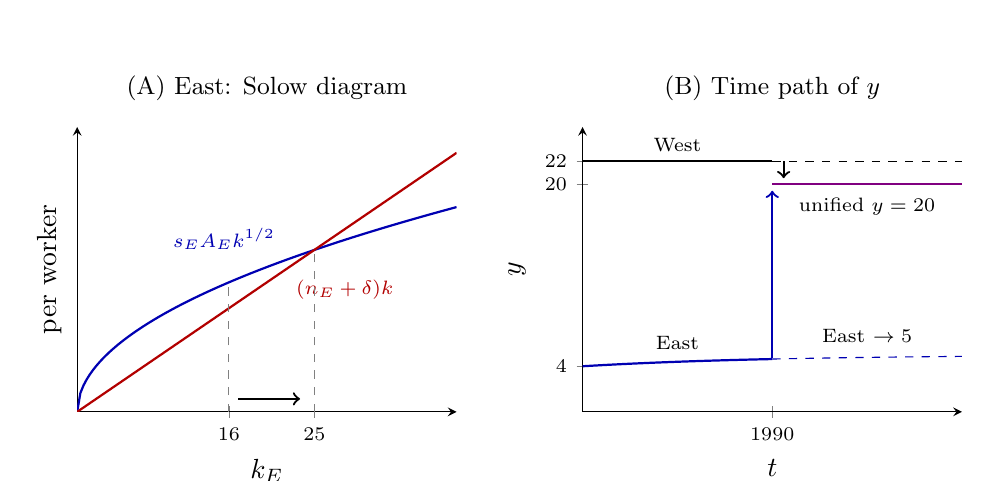
\begin{tikzpicture}
\begin{axis}[name=solow,width=6.4cm,height=5.2cm,axis lines=left,xmin=0,xmax=40,ymin=0,ymax=3.3,
  xlabel={$k_E$},ylabel={per worker},xtick={16,25},
  ytick=\empty,title={\small (A) East: Solow diagram},every tick label/.append style={font=\scriptsize}]
\addplot[domain=0:40,samples=120,thick,blue!70!black]{0.375*sqrt(x)} node[pos=0.55,above left,font=\scriptsize]{$s_EA_Ek^{1/2}$};
\addplot[domain=0:40,thick,red!70!black]{0.075*x} node[pos=0.55,below right,font=\scriptsize]{$(n_E+\delta)k$};
\draw[dashed,gray](axis cs:16,0)--(axis cs:16,1.5);
\draw[dashed,gray](axis cs:25,0)--(axis cs:25,1.875);
\draw[->,thick](axis cs:17,0.15)--(axis cs:23.5,0.15);
\end{axis}
\begin{axis}[at={(solow.east)},anchor=west,xshift=1.6cm,width=6.4cm,height=5.2cm,axis lines=left,
  xmin=-10,xmax=10,ymin=0,ymax=25,xlabel={$t$},ylabel={$y$},xtick={0},xticklabels={1990},
  ytick={4,20,22},title={\small (B) Time path of $y$},every tick label/.append style={font=\scriptsize}]
\addplot[thick,black]coordinates{(-10,22)(0,22)};
\addplot[dashed,black]coordinates{(0,22)(10,22)};
\addplot[domain=-10:0,samples=40,thick,blue!70!black]{5-exp(-0.1*(x+10))};
\addplot[domain=0:10,samples=40,dashed,blue!70!black]{5-exp(-0.1*(x+10))};
\addplot[thick,violet]coordinates{(0,20)(10,20)};
\draw[->,thick,blue!70!black](axis cs:0,4.7)--(axis cs:0,19.4);
\draw[->,thick,black](axis cs:0.6,22)--(axis cs:0.6,20.5);
\node[font=\scriptsize,anchor=south] at (axis cs:-5,22){West};
\node[font=\scriptsize,anchor=south] at (axis cs:-5,4.6){East};
\node[font=\scriptsize,anchor=south] at (axis cs:5,5.2){East $\to5$};
\node[font=\scriptsize,anchor=north] at (axis cs:5,19.6){unified $y=20$};
\end{axis}
\end{tikzpicture}\\
{\footnotesize Figure 1. (A) East starts below its own $k^*$. (B) Solid: actual paths; dashed: no-unification counterfactuals (schematic timing).}
\end{center}
\rubric{
\item Period-0 values: 1 pt. Steady-state formula and four numbers: 2 pts.
\item Direction for each region (West flat, East rising with falling growth): 1 pt.
\item Named \emph{conditional} convergence, gap in levels persists: 1 pt. Diagram with labelled curves, $k_0$, $k^*$: counts in this point if the words are missing.
\item Calling it ``divergence'' or ``absolute convergence'': max.\ 2 pts.
}
\end{sol}

\textbf{b)} (5 points) Unification: from 1990 all production uses West technology $A_W=2$ with the
pooled capital and labour of both regions. Compute the new $y$ and its change for West and for East
workers (in levels and in \% of the pre-unification value), and the change in aggregate German output
$Y$. Explain \emph{where} each region's gain or loss comes from.
\answerspace
\begin{sol}
\step{pooling}{$K=7744+256=8000$, $L=64+16=80\Rightarrow k_U=8000/80=100$, $y_U=2\sqrt{100}=\res{20}$.}
\step{per capita changes}{West: $22\to20$: $\res{-2,\ -9.09\%}$ (base 22). East: $4\to20$: $\res{+16,\ +400\%}$ (base 4).}
\step{West: source}{\textbf{Capital dilution}: same $A$, but $k$: $121\to100$ because East brings 20\% of the workers
and only 3.2\% of the capital. $K/L\downarrow\to y\downarrow$. Factor prices: $w=(1-\alpha)y$: $11\to10$ (West workers lose);
$r^K=\alpha y/k$: $1/11=0.091\to0.10$ (West capital owners gain).}
\step{East: source}{\textbf{Technology} $A:1\to2$ and \textbf{capital deepening} $k:16\to100$. Technology first:
$1\cdot4\to2\cdot4=8$ ($+4$), then capital $8\to20$ ($+12$). In logs (order-free):
$\ln5=\underbrace{\ln2}_{\text{technology}}+\underbrace{\tfrac12\ln(100/16)}_{\text{capital deepening}}=0.693+0.916$;
technology $\approx43\%$ of the log gain. $w_E$: $2\to10$.}
\step{aggregate}{Before: $Y=22\cdot64+4\cdot16=1408+64=1472$. After: $Y=20\cdot80=1600$.
$\Delta Y=\res{+128,\ +8.70\%}$. Germany-wide $y$: $1472/80=18.4\to20$. Source: East's $K$ and $L$ now work
with the better technology; West's loss per head is a \emph{redistribution} of capital, not lost output.}
\step{check}{$64\cdot(-2)+16\cdot(+16)=-128+256=128=\Delta Y$.}
\intuition{Per-capita and aggregate answers differ in sign for the West: West $y$ falls, yet German $Y$ rises.
``Not per capita for the West, but still an aggregate gain.''}
\refbib{Kurlat \S4.1--\S4.2, pp.~53--61; \S4.4, pp.~63--69 (factor prices).}
\rubric{
\item $k_U$, $y_U$ and the two per-capita changes with bases: 2 pts.
\item Sources: West = capital dilution (1 pt); East = technology + capital deepening (1 pt).
\item Aggregate $\Delta Y$ computed and interpreted: 1 pt.
\item Numbers with no source of gain/loss: max.\ 3 pts. Per capita only, no aggregate: max.\ 4 pts. Arithmetic slip: $-1$.
}
\end{sol}

\textbf{c)} (5 points) After unification Germany saves at the West's rate $s_W$ and its labour force
grows at the labour-weighted average of $n_W$ and $n_E$. Compute $k^*_U$ and $y^*_U$. Is unified
Germany below its steady state? Compare $y^*_U$ with $y^*_W$ and explain the difference.
\answerspace
\begin{sol}
\step{population growth}{$n_U=\dfrac{64\cdot0+16\cdot0.025}{80}=\dfrac{0.4}{80}=0.005$.}
\step{steady state}{$\dfrac{s_WA_W}{n_U+\delta}=\dfrac{0.55}{0.055}=10\Rightarrow\res{k^*_U=100,\ y^*_U=20}$.}
\step{position}{$k_U=100=k^*_U$: \res{\text{exactly at the steady state}} --- no transition; $y$ stays at 20,
$g_y=0$, and aggregate $Y$ grows at $n_U=0.5\%$.}
\step{comparison}{$y^*_U=20<y^*_W=22$ although $A$ and $s$ are the West's. The only difference is
$n_U=0.005>n_W=0$: break-even investment $(n+\delta)k$ is steeper ($0.055$ vs $0.05$), so each worker's capital
is diluted faster by newcomers and the same saving supports less $k$:
$n\uparrow\to(n+\delta)k\uparrow\to k^*\downarrow\to y^*\downarrow$.}
\intuition{Unification did not make the West's steady state unattainable because of the East's technology
(that was replaced) or its saving (not used): it is population growth alone. The 2-point gap is permanent,
unlike the 2-point loss in (b), which was a pure level redistribution.}
\refbib{Kurlat \S4.2, pp.~59--61; \S5.3, pp.~79--86 (convergence).}
\rubric{
\item $n_U$: 1 pt. $k^*_U$, $y^*_U$: 2 pts.
\item Position relative to SS: 1 pt. Explanation via $n$ and break-even investment: 1 pt.
\item Numbers with no explanation: max.\ 3 pts. Using unweighted $n$ ($0.0125$): $-1$ pt, rest graded on method.
}
\end{sol}
\begin{sol}
\gap{Lista 2, 1(b) (``divergence'' instead of conditional convergence); 1(c) (source of each region's gain/loss); 1(d) (numbers right, no explanation).}
\end{sol}

% =============================================================================
\block{III}{Microfoundations}{Lectures 4--6; Kurlat chs.~6, 7, 9 \,\textbullet\, 25 points}

\question{(10 points) Objective items.}

\textbf{a)} (3 points) A household has one unit of time, preferences $\ln c+\psi\ln l$ with $\psi=1$,
wage $w=10$, pays a tax $\tau$ on labour income and receives a lump-sum transfer $T=2$, so
$c=(1-\tau)w(1-l)+T$. The labour-income tax rises from $\tau=0.2$ to $\tau=0.5$ ($T$ unchanged). Hours:
\begin{options}
\item fall from 0.375 to 0.300: leisure became cheaper, an effect that would lower hours even with $T=0$.
\item stay at 0.500: with log utility the income and substitution effects cancel whatever $T$ is.
\item rise from 0.375 to 0.450: the lower net wage makes the household poorer, so it works more.
\item fall from 0.500 to 0.375: the tax lowers the price of leisure one-for-one with $\tau$.
\item fall from 0.375 to 0.300: the fixed $T$ grows relative to net earnings; with $T=0$ hours would not move.
\end{options}
\answer{E}
\begin{sol}
\step{labour supply}{MRS $=$ net wage: $\dfrac{\psi c}{l}=(1-\tau)w$ with $c=(1-\tau)w(1-l)+T$ $\Rightarrow$
$n=1-l=\dfrac{1}{1+\psi}-\dfrac{\psi T}{(1+\psi)(1-\tau)w}$. $\tau=0.2$: $0.5-\frac{2}{16}=0.375$; $\tau=0.5$: $0.5-\frac{2}{10}=0.300$.
With $T=0$, $n=0.5$ for any $\tau$: the effect runs only through $T$ (pure income effect), so A's reason is false.}
\refbib{Kurlat \S7.2, pp.~131--137.}
\gap{Lista 4, 1(b): the words described a substitution effect; the formula said the effect is through $T$.}
\end{sol}

\medskip
\textbf{b)} (3 points) In a search economy with $m(V,U)=\mu V^\alpha U^{1-\alpha}$, one firm posts one extra
vacancy. Which statement is correct?
\begin{options}
\item The posting firm and the other firms gain; unemployed workers lose, as matches per worker fall.
\item Unemployed workers gain ($f$ rises); other firms lose ($q$ falls); the posting firm gains privately.
\item The posting firm loses, because its own $q$ falls; this private cost is the congestion externality.
\item Everyone gains, since $m$ rises one-for-one with $V$, so the extra vacancy creates no externality.
\item Unemployed workers lose ($f$ falls); other firms gain ($q$ rises); the posting firm is unaffected.
\end{options}
\answer{B}
\begin{sol}
\step{signs}{$\theta=V/U\uparrow\Rightarrow f=\mu\theta^\alpha\uparrow$, $q=\mu\theta^{\alpha-1}\downarrow$; $\partial m/\partial V=\alpha q<q$
(not one-for-one: friction). The congestion cost lands on \emph{other} firms; the posting firm, which
expects profit, ignores both that cost and the benefit to workers.}
\refbib{Kurlat \S7.5, pp.~142--150.}
\gap{Lista 4, 2(d): externality placed on the posting firm itself.}
\end{sol}

\medskip
\textbf{c)} (2 points, T or F) A fall in matching efficiency $\mu$, which raises the vacancy rate
needed at every unemployment rate, is a movement along the Beveridge curve.
\answer{False}
\begin{sol}
\step{shift}{The Beveridge curve $s(1-u)=\mu v^\alpha u^{1-\alpha}$ (job destruction $=$ job creation) is drawn for a given
$\mu$. $\mu\downarrow$ moves every $(u,v)$ pair out: a \emph{shift}. A movement along it is a change in
tightness $\theta$ at given matching technology.}
\refbib{Kurlat \S7.1, pp.~127--131; \S7.5.}
\gap{Lista 4, 2(e): shift of vs movement along the Beveridge curve.}
\end{sol}

\medskip
\textbf{d)} (2 points, T or F) In the general-equilibrium economy with a fixed capital stock, no
investment, and preferences $\ln c+\psi\ln l$, a rise in TFP $A$ leaves hours worked unchanged.
\answer{True}
\begin{sol}
\step{equilibrium}{$\psi c/l=w$, $c=Y=AK^\alpha L^{1-\alpha}$, $w=(1-\alpha)AK^\alpha L^{-\alpha}$ $\Rightarrow$
$\psi\frac{L}{1-L}=1-\alpha\Rightarrow L=\frac{1-\alpha}{1-\alpha+\psi}$: no $A$. Equivalently
$\frac{d\ln L}{d\ln A}=\frac{1-\sigma}{\cdots}=0$ at $\sigma=1$: income and substitution effects cancel.}
\refbib{Kurlat \S9.1, pp.~165--168.}
\gap{Lista 5 (ungraded) and Lista 4, 1(b): with log utility, wage changes alone do not move hours.}
\end{sol}

% -----------------------------------------------------------------------------
\question{(15 points) A temporary tax cut financed by public debt. The Brazilian government
considers cutting this year's income tax and repaying the resulting debt next period. A household lives
two periods and solves
\[
\max_{c_1,c_2,a}\ u(c_1)+\beta u(c_2)\quad\text{s.t.}\quad c_1+a=y_1-\tau_1,\qquad c_2=y_2-\tau_2+(1+r)a,
\]
with $u(c)=\frac{c^{1-\sigma}}{1-\sigma}$ ($u=\ln c$ if $\sigma=1$), $\beta\in(0,1)$, $\sigma>0$. Baseline values:
$\sigma=1$, $\beta=0.8$, $r=0.25$ (a period is roughly a decade), $y_1=60$, $y_2=150$, $\tau_1=\tau_2=20$ (thousand reais).}

\textbf{a)} (5 points) By substituting the constraints into the objective (no Lagrangian needed), derive
the Euler equation and solve for $c_1$, $c_2$ and $a$ in closed form. Evaluate them at the baseline.
\answerspace
\begin{sol}
\step{substitute}{From period 1: $a=y_1-\tau_1-c_1$. Into period 2: $c_2=y_2-\tau_2+(1+r)(y_1-\tau_1-c_1)$.
Dividing by $1+r$: $c_1+\dfrac{c_2}{1+r}=\underbrace{y_1-\tau_1+\dfrac{y_2-\tau_2}{1+r}}_{\equiv\,W\ \text{(PV of after-tax income)}}$.}
\step{FOC}{$\max_{c_1}\ u(c_1)+\beta u\big(y_2-\tau_2+(1+r)(y_1-\tau_1-c_1)\big)$:\quad
$u'(c_1)-\beta(1+r)u'(c_2)=0\Rightarrow\res{c_1^{-\sigma}=\beta(1+r)\,c_2^{-\sigma}}$ (Euler: MRS $=1+r$).}
\step{solve}{$c_2=[\beta(1+r)]^{1/\sigma}c_1$. Into the PV constraint: $c_1\left[1+\beta^{1/\sigma}(1+r)^{\frac1\sigma-1}\right]=W$:
\[
\res{c_1=\frac{W}{D}},\quad \res{c_2=[\beta(1+r)]^{1/\sigma}\frac{W}{D}},\quad \res{a=y_1-\tau_1-\frac{W}{D}},\qquad
D\equiv1+\beta^{1/\sigma}(1+r)^{\frac1\sigma-1}.
\]}
\step{baseline}{$W=40+\frac{130}{1.25}=40+104=144$; $\sigma=1\Rightarrow D=1+\beta=1.8$.
$c_1=144/1.8=\res{80}$; $c_2=(0.8\cdot1.25)\cdot80=\res{80}$; $a=40-80=\res{-40}$ (borrows).}
\step{check}{$c_2=130+1.25\cdot(-40)=130-50=80$ \checkmark; Euler $1/80=0.8\cdot1.25/80$ \checkmark.}
\rubric{
\item Substitution and PV constraint: 1 pt. Euler equation: 1 pt.
\item Closed forms for $c_1,c_2$: 1 pt; \textbf{$a$ solved}: 1 pt. Baseline numbers: 1 pt.
\item Not solving for $a$: max.\ 4 pts. Lagrangian route is accepted. Arithmetic slip: $-1$.
}
\end{sol}

\textbf{b)} (5 points) Set $y_2=\tau_1=\tau_2=0$ (general $\sigma$). Compute $\partial c_1/\partial r$, isolate
the factor that determines its sign, and state, in words consistent with that sign, what happens to
$c_1$ when $r$ rises for $\sigma>1$, $\sigma=1$ and $\sigma<1$.
\answerspace
\begin{sol}
\step{set up}{$W=y_1$, so $c_1=\dfrac{y_1}{D(r)}$, $D(r)=1+\beta^{1/\sigma}(1+r)^{\frac{1-\sigma}{\sigma}}$.}
\step{differentiate}{$\dfrac{\partial D}{\partial r}=\beta^{1/\sigma}\,\dfrac{1-\sigma}{\sigma}\,(1+r)^{\frac{1-2\sigma}{\sigma}}$, so
\[
\frac{\partial c_1}{\partial r}=-\frac{y_1}{D^2}\frac{\partial D}{\partial r}
=\frac{y_1\,\beta^{1/\sigma}(1+r)^{\frac{1-2\sigma}{\sigma}}}{D^2}\cdot\underbrace{\frac{\sigma-1}{\sigma}}_{\text{determines the sign}}.
\]}
\step{sign}{$\res{\sigma>1:\ \partial c_1/\partial r>0}$;\quad $\res{\sigma=1:\ =0}$ ($c_1=y_1/(1+\beta)$);\quad $\res{\sigma<1:\ <0}$.}
\step{words}{The household is a pure saver. $r\uparrow$: \emph{substitution effect} --- $c_1$ is dearer in units of
$c_2$ $\to c_1\downarrow$; \emph{income effect} --- a saver is richer $\to c_1\uparrow$. $\sigma$ is the curvature of $u$;
$1/\sigma$ is the elasticity of intertemporal substitution. $\sigma>1$ (low EIS): income effect dominates,
so $c_1$ \textbf{rises} and saving falls. $\sigma<1$: substitution dominates, $c_1$ \textbf{falls}. $\sigma=1$: they cancel.}
\refbib{Kurlat \S6.2, pp.~112--115.}
\rubric{
\item $c_1(r)$ and correct derivative: 2 pts. Sign factor isolated: 1 pt.
\item Words matching the sign for each case (income vs substitution, saver): 2 pts.
\item Correct sign condition but words with the opposite direction (e.g.\ ``$\sigma>1$, $c_1$ falls''): max.\ 2 pts.
}
\end{sol}

\textbf{c)} (5 points) Return to the baseline. The government cuts $\tau_1$ by $\Delta=10$ and raises
$\tau_2$ by $(1+r)\Delta$. (i) Find the effect on $c_1$, $c_2$ and $a$. Does the timing of taxes matter?
(ii) Now the household faces a borrowing limit $a\ge-b$ with $b=20$. Find $c_1$, $c_2$, $a$ before and
after the same tax change. (iii) Give two concrete examples of Brazilian households for whom such a
limit is likely to bind.
\answerspace
\begin{sol}
\step{(i) PV of taxes}{$\tau_1'+\dfrac{\tau_2'}{1+r}=(\tau_1-\Delta)+\dfrac{\tau_2+(1+r)\Delta}{1+r}=\tau_1+\dfrac{\tau_2}{1+r}=36$:
$W$ unchanged $\Rightarrow$ $\res{\Delta c_1=\Delta c_2=0,\ \Delta a=+\Delta=+10}$.
Numbers: $\tau_1=10$, $\tau_2=20+12.5=32.5$; $W=50+117.5/1.25=50+94=144$; $c_1=c_2=80$; $a=50-80=-30$.
The household saves the whole cut to pay the future tax (Ricardian equivalence): \textbf{timing does not
matter}, only the PV of taxes.}
\step{(ii) before}{Desired $a=-40<-20$ $\Rightarrow$ limit binds: $a=-20$, $c_1=y_1-\tau_1+b=40+20=\res{60}$,
$c_2=130+1.25(-20)=130-25=\res{105}$. Euler becomes an inequality: $u'(c_1)=1/60>\beta(1+r)u'(c_2)=1/105$.}
\step{(ii) after}{Desired $a=-30<-20$: still binds. $a=-20$; $c_1=50+20=\res{70}$ ($+10=\Delta$);
$c_2=117.5-25=\res{92.5}$ ($-12.5=-(1+r)\Delta$). MPC out of the cut $=1$; timing \textbf{matters}.
(It keeps binding while $-40+\Delta<-20$, i.e.\ $\Delta<20$.)}
\step{(iii) examples}{(1) A young medical resident or university student with low income now and high
expected income later, and no collateral. (2) An informal worker (or someone with a negative record at
Serasa) whose income fell temporarily and who cannot borrow against future earnings.}
\begin{center}
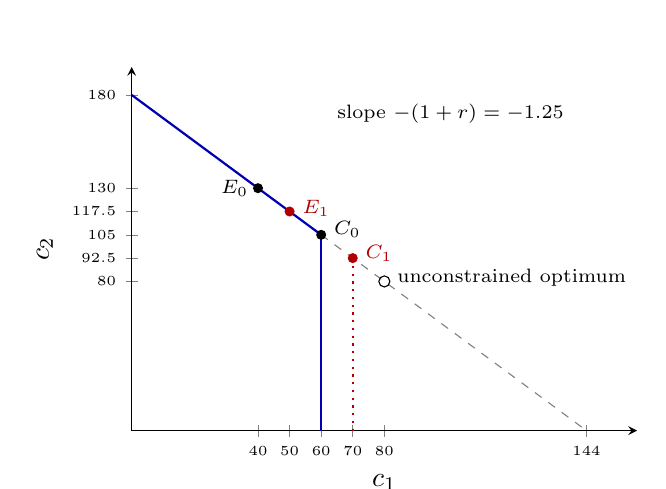
\begin{tikzpicture}
\begin{axis}[width=8cm,height=6.2cm,axis lines=left,xmin=0,xmax=160,ymin=0,ymax=195,
  xlabel={$c_1$},ylabel={$c_2$},xtick={40,50,60,70,80,144},ytick={80,92.5,105,117.5,130,180},
  every tick label/.append style={font=\tiny}]
\addplot[domain=60:144,dashed,gray]{1.25*(144-x)};
\addplot[domain=0:60,thick,blue!70!black]{1.25*(144-x)};
\draw[thick,blue!70!black](axis cs:60,105)--(axis cs:60,0);
\draw[dotted,thick,red!70!black](axis cs:70,92.5)--(axis cs:70,0);
\addplot[only marks,mark=*,mark size=1.6pt]coordinates{(40,130)(60,105)};
\addplot[only marks,mark=*,mark size=1.6pt,red!70!black]coordinates{(50,117.5)(70,92.5)};
\addplot[only marks,mark=o,mark size=2pt]coordinates{(80,80)};
\node[font=\scriptsize,anchor=east] at (axis cs:40,130){$E_0$};
\node[font=\scriptsize,anchor=west,red!70!black] at (axis cs:51,119){$E_1$};
\node[font=\scriptsize,anchor=west] at (axis cs:61,108){$C_0$};
\node[font=\scriptsize,anchor=west,red!70!black] at (axis cs:71,95){$C_1$};
\node[font=\scriptsize,anchor=west] at (axis cs:81,82){unconstrained optimum};
\node[font=\scriptsize,anchor=west] at (axis cs:62,170){slope $-(1+r)=-1.25$};
\end{axis}
\end{tikzpicture}\\
{\footnotesize Figure 2. The budget line is the same before and after the swap ($W=144$); the endowment slides
from $E_0$ to $E_1$ along it. The limit $c_1\le y_1-\tau_1+b$ moves from 60 to 70, so the constrained choice moves
from $C_0$ to $C_1$.}
\end{center}
\intuition{Ricardian equivalence needs the household to be able to move resources across periods at $r$.
When the limit binds, the tax cut is the loan the market would not give, and it is consumed one-for-one.}
\refbib{Kurlat \S6.2--\S6.4, pp.~120--126.}
\rubric{
\item (i) PV argument and $\Delta c_1=\Delta c_2=0$, $\Delta a=\Delta$: 2 pts.
\item (ii) Binding check and $c_1$ before/after: 1.5 pts (diagram with kink, labelled axes and points counts here).
\item (iii) Two examples: 1.5 pts (0.75 each).
\item Proving PV-only and then stating ``timing matters'' in the unconstrained case: max.\ 2 pts. One example only: $-0.75$.
}
\end{sol}
\begin{sol}
\gap{Lista 3, 1(a)(d) (never solved for $a$); 1(c) (right sign condition, opposite words); 1(e) (PV proved, then ``timing matters''); 2(b) (one example where two were asked).}
\end{sol}

% =============================================================================
\block{IV}{Money, inflation and AD--AS}{Lectures 7--9; Kurlat chs.~10--11; Benigno (2015) \,\textbullet\, 25 points}

\question{(10 points) Objective items.}

\textbf{a)} (3 points) About the quantity equation $MV=PY$:
\begin{options}
\item It is a theory of money demand: with $Y$ fixed, doubling $M$ doubles $P$ at every horizon.
\item It is an identity which proves neutrality, because $V$ and $Y$ are constant by definition.
\item It is a behavioural equation: $V$ is a structural parameter that the central bank sets.
\item It is an identity, since $V\equiv PY/M$; causation needs assumptions on $V$ and on what is exogenous.
\item It is an identity which proves causation runs from $P$ to $M$, because firms set prices first.
\end{options}
\answer{D}
\begin{sol}
\step{residual}{$V$ is measured as $PY/M$, so the equation holds for any data. It becomes a theory only with
an assumption on $V$ (e.g.\ stable, or given by a money-demand model) and on which variable is exogenous.}
\refbib{Kurlat \S10.4, pp.~199--204; \S11.2.}
\gap{Lista 6, 1(a): $V$ as a residual; causation needs an assumption.}
\end{sol}

\medskip
\textbf{b)} (3 points) In steady state with constant $i$, $\pi=\mu-\eta g$. The central bank targets $\pi^*=3\%$
with $g=2\%$ and sets $\mu$ assuming $\eta=1$ (Cambridge). Money demand is actually Baumol--Tobin. Inflation is:
\begin{options}
\item $2\%$
\item $3\%$
\item $4\%$
\item $5\%$
\item $6\%$
\end{options}
\answer{C}
\begin{sol}
\step{compute}{Chosen $\mu=\pi^*+1\cdot g=5\%$. Baumol--Tobin: $\eta=\tfrac12$, so $\pi=5\%-\tfrac12\cdot2\%=\res{4\%}$.
Desired real balances grow at $1\%$, not $2\%$: the extra money goes into prices.}
\refbib{Kurlat \S11.2, pp.~205--215.}
\gap{Lista 6, 2(b): inflation-targeting error formula.}
\end{sol}

\medskip
\textbf{c)} (2 points, T or F) When the central bank targets the nominal interest rate, the money-market
equilibrium $M=p\,m^D(Y,i)$ determines the quantity of money.
\answer{True}
\begin{sol}
\step{endogenous $M$}{With $i$ fixed by policy, and $p$, $Y$ given, $M$ must supply whatever $p\,m^D(Y,i)$ demands: the
central bank accommodates by open-market operations. Under a money target it is the reverse: $M$ given, $i$ adjusts.}
\refbib{Kurlat \S11.1--\S11.2; Benigno \S3 (policy sets $i$).}
\gap{Lista 6, 1(d): under an interest-rate target the money market determines $M$.}
\end{sol}

\medskip
\textbf{d)} (2 points, T or F) In Benigno's AD--AS model, a temporary rise in firms' desired mark-up
shifts the AD curve to the left.
\answer{False}
\begin{sol}
\step{which curve}{The mark-up enters the price-setting (AS) block: natural output falls, AS shifts up/left. AD comes
from the Euler equation and the policy rule, where $\mu$ does not appear: AD does not move (stagflation along AD).}
\refbib{Benigno (2015) \S4 and \S7.}
\gap{Shift of vs movement along AD/AS (taxonomy).}
\end{sol}

% -----------------------------------------------------------------------------
\question{(15 points) Pix and the demand for money. Since 2020 Pix, Brazil's instant-payment
system, has lowered the cost of turning deposits into means of payment. Model real money demand with
Baumol--Tobin, $m^D=\sqrt{\dfrac{FY}{2i}}$, where $F$ is the real cost of each conversion. Assume real
output grows at $g=2\%$, $F$ falls at the constant rate $\dot F/F=f=-4\%$, and $i$ is constant. The
money market clears: $M=p\,m^D(Y,i,F)$.}

\textbf{a)} (5 points) Derive velocity $V$ implied by this model. Explain why $V$ is not constant, and
compute its growth rate under the assumptions above. Interpret velocity in words.
\answerspace
\begin{sol}
\step{definition}{$V\equiv\dfrac{pY}{M}=\dfrac{pY}{p\,m^D}=\dfrac{Y}{\sqrt{FY/2i}}=\res{\sqrt{\dfrac{2iY}{F}}}$.}
\step{not constant}{$V$ depends on $i$ (opportunity cost of holding money $\uparrow\Rightarrow V\uparrow$), on $Y$
(economies of scale in cash management, $\partial\ln V/\partial\ln Y=\tfrac12$) and on $F$ (payment technology,
$\partial\ln V/\partial\ln F=-\tfrac12$).}
\step{growth}{$\dfrac{\dot V}{V}=\tfrac12\dfrac{\dot i}{i}+\tfrac12 g-\tfrac12 f=0+1\%+2\%=\res{3\%\ \text{per year}}$.}
\step{interpret}{$V$ is the number of times the average real balance is spent per period. In $MV=PY$ it
is a residual; Baumol--Tobin gives it a theory: cheaper conversions $\to$ smaller average balances per real
transaction $\to$ each real balance turns over faster.}
\refbib{Kurlat \S10.4, pp.~199--204.}
\rubric{
\item $V=\sqrt{2iY/F}$ derived: 2 pts.
\item Dependence on $i$, $Y$, $F$ with signs: 1 pt. Growth $3\%$: 1 pt. Interpretation: 1 pt.
\item Treating $V$ as constant or exogenous: max.\ 2 pts.
}
\end{sol}

\textbf{b)} (5 points) By totally differentiating $M=p\,m^D(Y,i,F)$ with respect to time, show that in
steady state $\pi=\mu-\tfrac12(g+f)$. Before Pix ($f=0$) the BCB grew money at the rate that delivered
$\pi=3\%$. Which money growth $\mu$ delivers $3\%$ after Pix? What inflation results if the BCB keeps the
old $\mu$? Explain the mechanism in words.
\answerspace
\begin{sol}
\step{differentiate}{$\dot M=\dot p\,m^D+p\left[\dfrac{\partial m^D}{\partial Y}\dot Y+\underbrace{\dfrac{\partial m^D}{\partial i}\dot i}_{=0\ (i\ \text{const.})}+\dfrac{\partial m^D}{\partial F}\dot F\right]$.}
\step{divide by $M=p\,m^D$}{$\mu=\pi+\underbrace{\dfrac{\partial m^D}{\partial Y}\dfrac{Y}{m^D}}_{\eta_Y}g+\underbrace{\dfrac{\partial m^D}{\partial F}\dfrac{F}{m^D}}_{\eta_F}f$.
From $m^D=(FY/2i)^{1/2}$: $\eta_Y=\eta_F=\tfrac12$ $\Rightarrow$ $\res{\pi=\mu-\tfrac12(g+f)}$.}
\step{before Pix}{$f=0$: $\mu=\pi^*+\tfrac12g=3\%+1\%=4\%$.}
\step{after Pix}{$\mu=\pi^*+\tfrac12(g+f)=3\%+\tfrac12(2\%-4\%)=3\%-1\%=\res{2\%}$.
Keeping $\mu=4\%$: $\pi=4\%-\tfrac12(-2\%)=\res{5\%}$.}
\step{mechanism}{$F\downarrow\to$ households hold smaller real balances $\to$ desired real money grows at
$\tfrac12(g+f)=-1\%$ instead of $+1\%$ $\to$ the same $\mu=4\%$ chases a \emph{shrinking} demand for real balances
$\to$ excess money $\to p$ grows faster: $\pi=5\%$. Equivalently, velocity rises at $3\%$. It is lower money
\emph{demand}, not ``cheap money''.}
\refbib{Kurlat \S11.2, pp.~205--215.}
\rubric{
\item Total differentiation with $\dot i=0$ struck: 1 pt. Elasticities named and $=\tfrac12$: 1 pt.
\item $\mu=2\%$ and $\pi=5\%$: 2 pts (1 each). Mechanism via money demand/velocity: 1 pt.
\item Explaining the effect as ``cheaper money'' or ``more money supply'': max.\ 3 pts. Arithmetic slip: $-1$.
}
\end{sol}

\textbf{c)} (5 points) Suppose instead the BCB sets the Selic (an interest-rate target $i^*$) and lets the
money supply be whatever it must be. When Pix lowers $F$, what adjusts in the money market in the short
run (prices sticky)? Is the Pix effect inflationary under this regime in the long run? Contrast with the
money-growth rule of (b).
\answerspace
\begin{sol}
\step{short run}{$F\downarrow\Rightarrow m^D\downarrow$ at every $i$ (curve shifts left). If $M$ stayed put, excess money
would push $i$ below $i^*$. To hold $i=i^*$ the BCB drains money (sells bonds):
$F\downarrow\to m^D\downarrow\to$ BCB sells bonds $\to M\downarrow$, $i=i^*$ unchanged $\to$ AD unchanged $\to y,p$ unchanged.
\res{\text{$M$ adjusts; $i$ does not.}}}
\step{long run}{$\pi$ is pinned by the target: $\pi=3\%$. Money growth becomes endogenous:
$\mu=\pi+\tfrac12(g+f)=3\%+\tfrac12(2\%-4\%)=\res{2\%}$. \res{\text{Not inflationary}}; Pix shows up only as slower
growth of money aggregates and rising velocity.}
\step{contrast}{Under a money-growth rule ($\mu=4\%$ fixed) the same shock raises $\pi$ to $5\%$, as in (b). The regime
decides whether a money-demand shock reaches prices: with an $i$ target the central bank absorbs it.}
\begin{center}
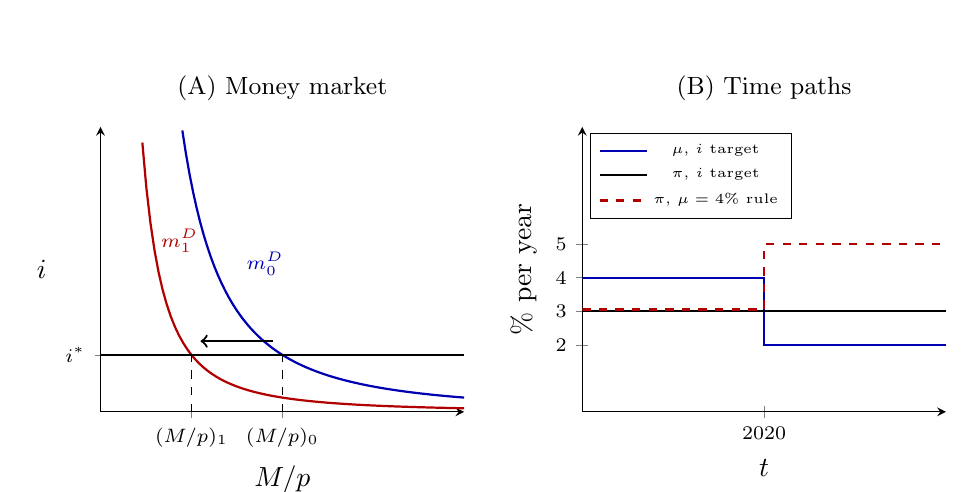
\begin{tikzpicture}
\begin{axis}[name=mm,width=6.2cm,height=5.2cm,axis lines=left,xmin=0,xmax=4,ymin=0,ymax=2.5,
  xlabel={$M/p$},ylabel={$i$},xtick={1,2},xticklabels={$(M/p)_1$,$(M/p)_0$},ylabel style={rotate=-90},ytick={0.5},yticklabels={$i^*$},
  title={\small (A) Money market},every tick label/.append style={font=\scriptsize}]
\addplot[domain=0.9:4,samples=80,thick,blue!70!black]{2/x^2};
\node[font=\scriptsize,blue!70!black,anchor=west] at (axis cs:1.5,1.3){$m^D_0$};
\addplot[domain=0.46:4,samples=80,thick,red!70!black]{0.5/x^2};
\node[font=\scriptsize,red!70!black] at (axis cs:0.87,1.5){$m^D_1$};
\addplot[thick,black]coordinates{(0,0.5)(4,0.5)};
\draw[dashed](axis cs:2,0)--(axis cs:2,0.5);
\draw[dashed](axis cs:1,0)--(axis cs:1,0.5);
\draw[->,thick](axis cs:1.9,0.62)--(axis cs:1.1,0.62);
\end{axis}
\begin{axis}[at={(mm.east)},anchor=west,xshift=1.5cm,width=6.2cm,height=5.2cm,axis lines=left,
  xmin=-5,xmax=5,ymin=0,ymax=8.5,xlabel={$t$},ylabel={\% per year},xtick={0},xticklabels={2020},
  ytick={2,3,4,5},title={\small (B) Time paths},every tick label/.append style={font=\scriptsize},
  legend style={font=\tiny,at={(0.02,0.98)},anchor=north west}]
\addplot[thick,blue!70!black]coordinates{(-5,4)(0,4)(0,2)(5,2)};
\addlegendentry{$\mu$, $i$ target}
\addplot[thick,black]coordinates{(-5,3)(5,3)};
\addlegendentry{$\pi$, $i$ target}
\addplot[dashed,thick,red!70!black]coordinates{(-5,3.05)(0,3.05)(0,5)(5,5)};
\addlegendentry{$\pi$, $\mu=4\%$ rule}
\end{axis}
\end{tikzpicture}\\
{\footnotesize Figure 3. (A) Lower $F$ shifts money demand left from $m^D_0=m^D(F_0)$ to $m^D_1=m^D(F_1)$ (drawn for $F_1=F_0/4$, which halves $m^D$); at $i^*$ real balances fall from $(M/p)_0$ to $(M/p)_1$.
(B) Under the $i$ target $\mu$ falls from 4\% to 2\% and $\pi$ stays at 3\%; under a fixed $\mu=4\%$, $\pi$ rises to 5\%.}
\end{center}
\intuition{Money is endogenous under an interest-rate rule: the central bank supplies the money people want at $i^*$.
A payment innovation that lowers money demand therefore changes $M$, not $i$, and leaves AD and inflation alone.}
\refbib{Kurlat \S11.1--\S11.2, pp.~205--215; Benigno (2015) \S3 (the central bank sets $i$).}
\rubric{
\item Short run: $m^D$ shifts left, $M$ adjusts, $i$ unchanged, no AD effect: 2 pts (arrow chain or diagram with labelled axes, curves and shift direction).
\item Long run: $\pi$ anchored, $\mu$ endogenous $=2\%$: 2 pts. Contrast with the money rule: 1 pt.
\item Stating that the BCB keeps $M$ fixed (or that $i$ falls) under an $i$ target: max.\ 2 pts.
}
\end{sol}
\begin{sol}
\gap{Lista 6, 1(a)(b) ($V$ a residual, velocity interpreted); 1(c) (mechanism; flexible-price neutrality: in the long run only $\pi$ and nominal aggregates move); 1(d) ($M$ endogenous under an $i$ target); 2(c) (falling $F$ = lower money demand, not ``cheap money'').}
\end{sol}

\end{document}
"
% Check fonts afterwards: pdffonts simulado-01-solutions.pdf  (all Type 1)
% Every number in the key is verified by simulado_codigo/check_simulado_01.py
% =============================================================================
\documentclass[11pt,a4paper]{article}
\usepackage[utf8]{inputenc}
\usepackage[T1]{fontenc}
\usepackage{lmodern}   % Type 1 vector fonts (replaces PK bitmaps)
\usepackage{cmap}      % ToUnicode CMap -> copyable text
\usepackage[english]{babel}
\usepackage{amsmath,amssymb,amsfonts}
\usepackage[a4paper,margin=2.2cm]{geometry}
\usepackage{enumitem}
\usepackage{fancyhdr}
\usepackage{comment}
\def\CommentCutFile{simulado-01.cut} % private cut file: sibling sources build in this folder
\usepackage{xcolor}
\usepackage{booktabs}
\usepackage{microtype}
\usepackage{pgfplots}
\pgfplotsset{compat=1.16}

% ====================== CONFIGURATION ======================
\newif\ifsolucoes
\ifdefined\withsolutions\solucoestrue\else\solucoesfalse\fi

\newcommand{\course}{Macroeconomics I --- MPE Insper}
\newcommand{\examtitle}{Mock Final Exam 1 (Simulado 1)}
\newcommand{\answerheight}{5.2cm}

% ====================== MACHINERY ======================
\ifsolucoes\includecomment{sol}\else\excludecomment{sol}\fi

\pagestyle{fancy}\fancyhf{}
\lhead{\footnotesize\course}
\rhead{\footnotesize\examtitle\ifsolucoes{} --- Solutions and Rubric\fi}
\cfoot{\footnotesize\thepage}
\renewcommand{\headrulewidth}{0.3pt}
\setlength{\headheight}{14pt}

\setlist{topsep=2pt,itemsep=2pt}
\newcounter{questao}

\newcommand{\block}[3]{\bigskip\noindent
  {\large\bfseries\color{blue!55!black}Block #1 --- #2}\par\noindent{\small\textit{(#3)}}\par
  \noindent\rule{\linewidth}{0.3pt}\smallskip}
\newcommand{\question}[1]{\refstepcounter{questao}\medskip\noindent
  \textbf{Question \thequestao.}~#1\par}
\newenvironment{options}{\begin{enumerate}[label=\Alph*.,leftmargin=2.2em,topsep=1pt]}{\end{enumerate}}
\newcommand{\answer}[1]{\ifsolucoes\par\noindent\textbf{Answer:}~#1\fi}
\newcommand{\answerspace}{\ifsolucoes\else\par\textit{Solution:}\vspace{\answerheight}\par\fi}
\newcommand{\step}[2]{\par\smallskip\noindent\textbf{Step --- #1.}~#2}
\newcommand{\intuition}[1]{\par\smallskip\noindent\textit{Intuition.}~#1}
\newcommand{\refbib}[1]{\par\smallskip\noindent{\footnotesize\color{black!60}\textbf{Ref:} #1}}
\newcommand{\gap}[1]{\par\smallskip\noindent{\footnotesize\color{red!55!black}\textbf{Gap targeted:} #1}}
\newcommand{\rubric}[1]{\par\smallskip\noindent\textbf{Rubric.}\begin{itemize}[leftmargin=1.4em,topsep=1pt]#1\end{itemize}}
\newcommand{\res}[1]{\boxed{#1}}

% =============================================================================
\begin{document}
\begin{center}
  {\Large\bfseries \course}\\[2pt]
  {\large \examtitle}\ifsolucoes\\[2pt]\textit{Solutions and Grading Rubric}\fi
\end{center}
\vspace{2pt}

{\footnotesize\noindent\textbf{Instructions.} Four blocks of 25 points each (100 points).
Suggested time: 3 hours. Multiple-choice items: mark the single correct option (no penalty
for wrong answers). \emph{True/False} items: every 2 wrong items cancel 1 right item
(score $=\max\{0,\ \text{right}-\text{wrong}/2\}\times$ item value); blank items do not
count as wrong. Discursive questions: show every step; box your final answers. Numerical
values are illustrative. Notation follows Kurlat (2020).\par}

% =============================================================================
\block{I}{Measurement}{Lecture 1; Kurlat chs.~1--2 \,\textbullet\, 25 points}

\question{(10 points) Objective items.}

\textbf{a)} (3 points) An economy produces two goods. In Year~1, good $X$ costs 10 and
$10$ units are produced; good $Z$ costs 5 and $20$ units are produced. In Year~2, $X$ costs 5
and $20$ units are produced; $Z$ costs 10 and $16$ units are produced. Real GDP growth from
Year~1 to Year~2 measured at Year-1 prices and at Year-2 prices is, respectively:
\begin{options}
\item $40\%$ at Year-1 prices; $4\%$ at Year-2 prices.
\item $4\%$ at Year-1 prices; $40\%$ at Year-2 prices.
\item $30\%$ at Year-1 prices; $30\%$ at Year-2 prices.
\item $40\%$ at Year-1 prices; $30\%$ at Year-2 prices.
\item $20.7\%$ at Year-1 prices; $20.7\%$ at Year-2 prices.
\end{options}
\answer{A}
\begin{sol}
\step{compute}{Nominal: $Y_1=10\cdot10+5\cdot20=200$, $Y_2=5\cdot20+10\cdot16=260$.
Year-2 output at Year-1 prices: $10\cdot20+5\cdot16=280\Rightarrow 280/200-1=\res{40\%}$.
Year-1 output at Year-2 prices: $5\cdot10+10\cdot20=250\Rightarrow 260/250-1=\res{4\%}$.
C is nominal growth ($260/200-1$), E is the Fisher index ($\sqrt{1.40\cdot1.04}-1$), B swaps the bases.}
\refbib{Kurlat \S1.2, pp.~22--25.}
\gap{Lista 1, 1(b)(c): Laspeyres/Paasche arithmetic slips.}
\end{sol}

\medskip
\textbf{b)} (3 points) Why is the GDP of a low-income country, converted into dollars at the
market exchange rate, systematically \emph{lower} than the same GDP converted at purchasing
power parity (PPP)?
\begin{options}
\item Tariffs and transport costs keep traded-goods prices apart across countries, and the market rate cannot close that gap.
\item Non-traded goods and services are cheap where wages are low, and the market rate, set by traded goods, ignores this.
\item The market rate is driven by capital flows rather than by trade, so it undervalues every poor-country currency by the same factor.
\item Large informal sectors are left out of the official statistics, so a big share of production is missing from measured GDP.
\item Quotas and import licences raise traded-goods prices in poor countries, which inflates their measured price level.
\end{options}
\answer{B}
\begin{sol}
\step{mechanism}{The market rate equalises (roughly) the prices of \emph{traded} goods. Non-traded
output (housing, haircuts, public services) is priced off local wages, which are low where
productivity in tradables is low (Balassa--Samuelson). Converting at the market rate values that
output at rich-country prices nobody there pays $\Rightarrow$ understates real output. A and E are
frictions in traded goods (and E goes the wrong way); D lowers GDP at \emph{any} conversion rate, so it
cannot explain the gap between the two; C has no mechanism.}
\refbib{Kurlat \S1.2, pp.~25--27.}
\gap{Lista 1, 1(e): PPP gap explained with trade costs instead of non-tradables.}
\end{sol}

\medskip
\textbf{c)} (2 points, T or F) In a two-good economy, if between two years quantities shift
toward the good whose relative price fell, then real GDP growth measured at initial-year prices
exceeds real GDP growth measured at final-year prices.
\answer{True}
\begin{sol}
\step{proof}{With goods $x,z$: $\sum p^0q^1\cdot\sum p^1q^0-\sum p^0q^0\cdot\sum p^1q^1
=(q^1_xq^0_z-q^0_xq^1_z)(p^0_xp^1_z-p^0_zp^1_x)$. The first factor is $>0$ iff quantities moved toward
$x$; the second is $>0$ iff the relative price of $x$ fell. Both hold $\Rightarrow$ Laspeyres growth $>$
Paasche growth (substitution bias). Item (a) is an instance: 40\% $>$ 4\%.}
\refbib{Kurlat \S1.2, pp.~22--25.}
\gap{Lista 1, 1(c): direction of the substitution bias not explained.}
\end{sol}

\medskip
\textbf{d)} (2 points, T or F) Brazil imports all the smartphones it consumes and produces none.
A rise in their dollar price raises the IPCA and the GDP deflator by the same proportion, since both
measure ``the price level''.
\answer{False}
\begin{sol}
\step{coverage}{The GDP deflator $=P Y^{\text{nominal}}/Y^{\text{real}}$ covers only goods
\emph{produced} in Brazil; imports are subtracted in $Y=C+I+G+X-M$. The IPCA prices a consumer basket,
imported goods included. So the IPCA rises and the deflator does not move.}
\refbib{Kurlat \S1.2, pp.~22--25.}
\gap{Deflator vs CPI (taxonomy of \texttt{rules/00\_estilo\_avaliacao.md}); reciprocal trap.}
\end{sol}

% -----------------------------------------------------------------------------
\question{(15 points) IBGE and the smartphone boom. Consider a stylised Brazil producing only
soybeans ($s$) and smartphones ($m$). Values in billions of reais; population in millions.}

\begin{center}
\begin{tabular}{lcccc c}
\toprule
 & $p_s$ & $q_s$ & $p_m$ & $q_m$ & Population \\
\midrule
2015 & 10 & 60 & 20 & 20 & 200 \\
2025 & 12 & 60 & 12 & 40 & 210 \\
\bottomrule
\end{tabular}
\end{center}

\textbf{a)} (5 points) Compute nominal GDP in both years; real GDP in 2015 prices and in 2025
prices; the real growth rate between 2015 and 2025 in each base; and the Fisher (chained) growth
rate. State which year's value is in the denominator of each rate.
\answerspace
\begin{sol}
\step{nominal}{$PY_{2015}=10\cdot60+20\cdot20=600+400=\res{1000}$;\;
$PY_{2025}=12\cdot60+12\cdot40=720+480=\res{1200}$. Nominal growth $1200/1000-1=20\%$.}
\step{base 2015 (Laspeyres)}{$Y_{2025}^{(2015)}=10\cdot60+20\cdot40=600+800=1400$;\;
$Y_{2015}^{(2015)}=1000$.\; $g=\dfrac{1400}{1000}-1=\res{40\%}$ (2015 value in the denominator).}
\step{base 2025 (Paasche)}{$Y_{2015}^{(2025)}=12\cdot60+12\cdot20=720+240=960$;\;
$Y_{2025}^{(2025)}=1200$.\; $g=\dfrac{1200}{960}-1=0.25=\res{25\%}$ (2015 value, at 2025 prices, in the denominator).}
\step{Fisher}{$1+g_F=\sqrt{1.40\times1.25}=\sqrt{1.75}=1.3229\Rightarrow\res{g_F=32.29\%}$. With two years
the chain has one link, so chained $=$ Fisher.}
\step{check}{$25\%<32.29\%<40\%$: the geometric mean lies between the two bases.
Implied deflator: $1200/1400=0.857$ (base 2015).}
\rubric{
\item Nominal GDP, both years: 1 pt.
\item Real GDP in both bases and the two growth rates: 2 pts (1 each).
\item Fisher: 1 pt. Denominators stated: 1 pt.
\item Arithmetic slip with correct method: $-1$ pt (once). Swapping the bases (40\% at 2025 prices): max.\ 2 pts.
}
\end{sol}

\textbf{b)} (5 points) The two bases give different answers. For each one, say whether it
overstates or understates growth relative to the Fisher index, and explain \emph{why}, using the
movement of relative prices and quantities in the table.
\answerspace
\begin{sol}
\step{what moved}{Relative price $p_m/p_s$: $20/10=2\ \to\ 12/12=1$ (smartphones got \emph{cheaper}).
Quantities: $q_s$ constant, $q_m$: $20\to40$. Quantities moved \emph{toward} the good whose relative price fell.}
\step{2015 prices}{The 20 extra smartphones are valued at the \emph{old, high} price 20: the gain is $20\cdot20=400$
on a base of 1000 $\Rightarrow$ 40\% $\Rightarrow$ \res{\text{overstates}}.}
\step{2025 prices}{The same 20 phones are valued at the \emph{new, low} price 12: gain $12\cdot20=240$ on 960
$\Rightarrow$ 25\% $\Rightarrow$ \res{\text{understates}}.}
\step{name}{Arrow chain: $p_m/p_s\downarrow\ \to\ q_m/q_s\uparrow$ (substitution) $\to$ fast-growing good weighted
at its high old price (Laspeyres $\uparrow$) or at its low new price (Paasche $\downarrow$). This is
\textbf{substitution bias}; statistical agencies (IBGE included) chain the index with
previous-year prices to shrink it.}
\intuition{Both numbers are correct arithmetic; they answer ``how much more output, valued at which prices?''.
An observer who sees only one base would wrongly attribute the difference to real performance. The bias is
not a convention: its sign is fixed by the negative co-movement of prices and quantities.}
\refbib{Kurlat \S1.2, pp.~22--25.}
\rubric{
\item Relative price and quantity movements identified: 1 pt.
\item Direction of each bias: 2 pts (1 each).
\item Cause (valuing the fast-growing good at high vs low price; substitution bias named): 2 pts.
\item ``The base year is a convention'' with no direction or cause: max.\ 1 pt.
}
\end{sol}

\textbf{c)} (5 points) Compute real GDP growth per capita in each base and with Fisher. Which
number, aggregate or per capita, answers ``did the average Brazilian become better off?''
and which answers ``how much bigger is the Brazilian economy?'' What does neither answer?
\answerspace
\begin{sol}
\step{population}{$n=210/200-1=5\%$. Per capita: $1+g_y=\dfrac{1+g_Y}{1+n}$.}
\step{per capita}{2015 prices: $1.40/1.05-1=\res{33.33\%}$; 2025 prices: $1.25/1.05-1=\res{19.05\%}$;
Fisher: $1.3229/1.05-1=\res{25.99\%}$.}
\step{levels}{Per capita 2015: $1000/200=5$ thousand reais; 2025 at 2015 prices: $1400/210=6.67$.}
\step{interpret}{Aggregate ($32.29\%$ Fisher): size of the economy, tax base, market size.
Per capita ($25.99\%$): average living standard $\Rightarrow$ the welfare question. Neither measures
consumption vs.\ investment, leisure, distribution or non-market output (Kurlat ch.~2: GDP per
capita is a proxy for welfare, not welfare).}
\rubric{
\item Correct formula $(1+g_Y)/(1+n)$: 1 pt; three per-capita rates: 2 pts.
\item Aggregate vs per capita matched to the two questions: 1 pt. Limits of GDP per capita: 1 pt.
\item Answering only per capita (or only aggregate): max.\ 2 pts. Subtracting $n$ instead of dividing: $-1$ pt only if stated as exact.
}
\end{sol}
\begin{sol}
\refbib{Kurlat \S1.2, pp.~22--27; \S2.1--\S2.2, pp.~31--44.}
\gap{Lista 1, 1(b)(c) (arithmetic and direction of substitution bias); Lista 1, 4(a) (aggregate and per capita both asked).}
\end{sol}

% =============================================================================
\block{II}{Growth and the Solow model}{Lectures 2--3; Kurlat chs.~3--5 \,\textbullet\, 25 points}

\question{(10 points) Objective items. Items (a)--(b) use the Solow model in per-worker terms,
$y=Ak^\alpha$, with no technological progress, $A=1$, $\alpha=1/3$, $s=0.24$, $n=0.01$, $\delta=0.05$,
and $(1+n)k_{t+1}=(1-\delta)k_t+sAk_t^\alpha$.}

\textbf{a)} (3 points) Steady-state capital per worker $k^*$ is:
\begin{options}
\item $2$
\item $4$
\item $8$
\item $10.52$
\item $64$
\end{options}
\answer{C}
\begin{sol}
\step{SS}{$(n+\delta)k=sAk^\alpha\Rightarrow k^*=\left(\dfrac{sA}{n+\delta}\right)^{\frac1{1-\alpha}}=\left(\dfrac{0.24}{0.06}\right)^{3/2}=4^{3/2}=\res{8}$.
A is $y^*=8^{1/3}=2$; B omits the exponent; D omits $n$ ($4.8^{3/2}$); E uses exponent $1/\alpha$.}
\refbib{Kurlat \S4.2, pp.~59--61.}
\gap{Level of $k$ vs level of $y$; break-even investment includes $n$.}
\end{sol}

\medskip
\textbf{b)} (3 points) About the Golden-Rule saving rate $s_{gold}$ of this economy:
\begin{options}
\item $s_{gold}=0.24$; the economy is already at the Golden Rule and $c^*$ cannot rise.
\item $s_{gold}=1$; saving all output maximises $k^*$ and therefore also maximises $c^*$.
\item $s_{gold}=2/3$; it equals the labour share, so raising $s$ to $2/3$ maximises $c^*$.
\item $s_{gold}=1/3$; raising $s$ from $0.24$ toward it raises $c^*$ in the long run.
\item $s_{gold}=1/3$; raising $s$ from $0.24$ lowers $c^*$, as the economy is dynamically inefficient.
\end{options}
\answer{D}
\begin{sol}
\step{golden rule}{$\max_s c^*=(1-s)Ak^{*\alpha}$ $\Leftrightarrow f'(k)=n+\delta$ $\Leftrightarrow s_{gold}=\alpha=1/3$.
With $s=0.24<1/3$: $c^*(0.24)=0.76\cdot2=1.52<c^*(1/3)=\tfrac23\sqrt{1/3/0.06}=1.571$. Below the Golden
Rule the economy is dynamically \emph{efficient}; the long-run gain costs consumption during the transition.}
\refbib{Kurlat \S4.3, pp.~61--63.}
\gap{SS saving vs Golden Rule confusion (taxonomy).}
\end{sol}

\medskip
\textbf{c)} (2 points, T or F) In the Solow model without technological progress, a permanently
higher saving rate raises the long-run growth rate of output per worker.
\answer{False}
\begin{sol}
\step{level vs rate}{$s\uparrow\Rightarrow k^*,y^*\uparrow$ (level), growth is positive only during the
transition; in the new steady state $g_y=0$ again. Long-run growth of $y$ requires technological progress.}
\refbib{Kurlat \S4.2, pp.~59--61.}
\gap{Lista 2, 1(b): what the model predicts about growth rates vs levels.}
\end{sol}

\medskip
\textbf{d)} (2 points, T or F) Starting from a steady state, a permanent fall in population growth
$n$ raises $k^*$ and temporarily raises the growth rate of output per worker above its steady-state rate.
\answer{True}
\begin{sol}
\step{mechanism}{$n\downarrow\Rightarrow$ break-even line $(n+\delta)k$ flatter $\Rightarrow k^*\uparrow$. At the old
$k^*$, $sAk^\alpha>(n+\delta)k$ $\Rightarrow k\uparrow, y\uparrow$: $g_y>0$ during convergence, back to $0$ in SS.
(Aggregate $Y$ grows \emph{more slowly} in the new SS: $g_Y=n$.)}
\refbib{Kurlat \S4.2, pp.~59--61.}
\gap{Lista 1, 4(b) (left blank): ``higher level, lower SS growth, higher growth during convergence''.}
\end{sol}

% -----------------------------------------------------------------------------
\question{(15 points) German reunification, 1990. Treat West ($W$) and East ($E$) Germany as two
closed Solow economies without technological progress, $Y_i=A_iK_i^{\alpha}L_i^{1-\alpha}$ with a common
$\alpha=1/2$ and $\delta=0.05$, and $(1+n_i)k_{i,t+1}=(1-\delta)k_{i,t}+s_iA_ik_{i,t}^{\alpha}$, where $k=K/L$ and
$y=Y/L$ (per worker $=$ per capita). Units: $L$ in millions, $K$ in index units.}

\begin{center}
\begin{tabular}{lccccc}
\toprule
 & $A_i$ & $s_i$ & $n_i$ & $L_{i,0}$ & $K_{i,0}$ \\
\midrule
West & 2 & 0.275 & 0 & 64 & 7744 \\
East & 1 & 0.375 & 0.025 & 16 & 256 \\
\bottomrule
\end{tabular}
\end{center}

\textbf{a)} (5 points) Compute $k$ and $y$ in each region in period 0, and each region's steady
state $k^*_i$, $y^*_i$. What does the model predict about growth in each region, and about the gap
between them? Name the prediction.
\answerspace
\begin{sol}
\step{period 0}{$k_W=7744/64=\res{121}$, $y_W=2\sqrt{121}=\res{22}$;\quad $k_E=256/16=\res{16}$, $y_E=1\cdot\sqrt{16}=\res{4}$.}
\step{steady state}{Set $k_{t+1}=k_t$: $(1+n)k=(1-\delta)k+sAk^\alpha\Rightarrow(n+\delta)k=sAk^\alpha\Rightarrow
k^*=\left(\dfrac{sA}{n+\delta}\right)^{\frac1{1-\alpha}}=\left(\dfrac{sA}{n+\delta}\right)^2.$\\
West: $\dfrac{0.275\cdot2}{0.05}=11\Rightarrow\res{k^*_W=121,\ y^*_W=22}$.\quad
East: $\dfrac{0.375\cdot1}{0.075}=5\Rightarrow\res{k^*_E=25,\ y^*_E=5}$.}
\step{dynamics}{West: $k_W=k^*_W\Rightarrow g_y=0$, and $Y_W$ constant ($n_W=0$). East: $k_E=16<25\Rightarrow
k\uparrow,\ y\uparrow$, e.g.\ $k_{E,1}=\frac{0.95\cdot16+0.375\cdot4}{1.025}=\frac{16.7}{1.025}=16.29$,
$y_{E,1}=4.036$ ($+0.91\%$); the growth rate falls as $k\to25$. Aggregate $Y_E$ grows at $g_y+n_E$, tending to $2.5\%$.}
\step{prediction}{\res{\text{Conditional convergence}}: East grows faster than West \emph{now}, but each
converges to its \emph{own} steady state. $y^*_E/y^*_W=5/22=22.7\%$: the level gap persists (from $4/22=18.2\%$),
because $A_E<A_W$ and $n_E>n_W$ outweigh $s_E>s_W$. Not divergence, and not absolute convergence.}
\step{diagram}{Figure 1: mechanism (left) and time path (right).}
\begin{center}
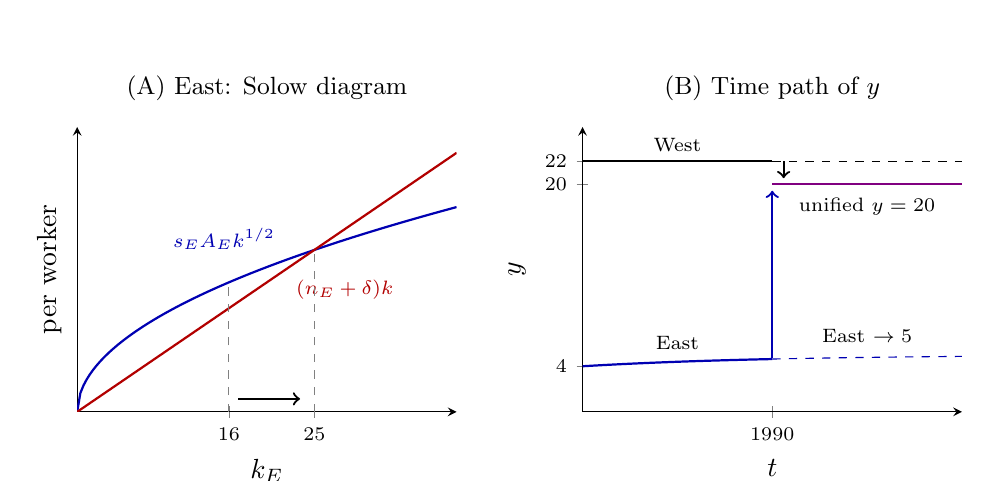
\begin{tikzpicture}
\begin{axis}[name=solow,width=6.4cm,height=5.2cm,axis lines=left,xmin=0,xmax=40,ymin=0,ymax=3.3,
  xlabel={$k_E$},ylabel={per worker},xtick={16,25},
  ytick=\empty,title={\small (A) East: Solow diagram},every tick label/.append style={font=\scriptsize}]
\addplot[domain=0:40,samples=120,thick,blue!70!black]{0.375*sqrt(x)} node[pos=0.55,above left,font=\scriptsize]{$s_EA_Ek^{1/2}$};
\addplot[domain=0:40,thick,red!70!black]{0.075*x} node[pos=0.55,below right,font=\scriptsize]{$(n_E+\delta)k$};
\draw[dashed,gray](axis cs:16,0)--(axis cs:16,1.5);
\draw[dashed,gray](axis cs:25,0)--(axis cs:25,1.875);
\draw[->,thick](axis cs:17,0.15)--(axis cs:23.5,0.15);
\end{axis}
\begin{axis}[at={(solow.east)},anchor=west,xshift=1.6cm,width=6.4cm,height=5.2cm,axis lines=left,
  xmin=-10,xmax=10,ymin=0,ymax=25,xlabel={$t$},ylabel={$y$},xtick={0},xticklabels={1990},
  ytick={4,20,22},title={\small (B) Time path of $y$},every tick label/.append style={font=\scriptsize}]
\addplot[thick,black]coordinates{(-10,22)(0,22)};
\addplot[dashed,black]coordinates{(0,22)(10,22)};
\addplot[domain=-10:0,samples=40,thick,blue!70!black]{5-exp(-0.1*(x+10))};
\addplot[domain=0:10,samples=40,dashed,blue!70!black]{5-exp(-0.1*(x+10))};
\addplot[thick,violet]coordinates{(0,20)(10,20)};
\draw[->,thick,blue!70!black](axis cs:0,4.7)--(axis cs:0,19.4);
\draw[->,thick,black](axis cs:0.6,22)--(axis cs:0.6,20.5);
\node[font=\scriptsize,anchor=south] at (axis cs:-5,22){West};
\node[font=\scriptsize,anchor=south] at (axis cs:-5,4.6){East};
\node[font=\scriptsize,anchor=south] at (axis cs:5,5.2){East $\to5$};
\node[font=\scriptsize,anchor=north] at (axis cs:5,19.6){unified $y=20$};
\end{axis}
\end{tikzpicture}\\
{\footnotesize Figure 1. (A) East starts below its own $k^*$. (B) Solid: actual paths; dashed: no-unification counterfactuals (schematic timing).}
\end{center}
\rubric{
\item Period-0 values: 1 pt. Steady-state formula and four numbers: 2 pts.
\item Direction for each region (West flat, East rising with falling growth): 1 pt.
\item Named \emph{conditional} convergence, gap in levels persists: 1 pt. Diagram with labelled curves, $k_0$, $k^*$: counts in this point if the words are missing.
\item Calling it ``divergence'' or ``absolute convergence'': max.\ 2 pts.
}
\end{sol}

\textbf{b)} (5 points) Unification: from 1990 all production uses West technology $A_W=2$ with the
pooled capital and labour of both regions. Compute the new $y$ and its change for West and for East
workers (in levels and in \% of the pre-unification value), and the change in aggregate German output
$Y$. Explain \emph{where} each region's gain or loss comes from.
\answerspace
\begin{sol}
\step{pooling}{$K=7744+256=8000$, $L=64+16=80\Rightarrow k_U=8000/80=100$, $y_U=2\sqrt{100}=\res{20}$.}
\step{per capita changes}{West: $22\to20$: $\res{-2,\ -9.09\%}$ (base 22). East: $4\to20$: $\res{+16,\ +400\%}$ (base 4).}
\step{West: source}{\textbf{Capital dilution}: same $A$, but $k$: $121\to100$ because East brings 20\% of the workers
and only 3.2\% of the capital. $K/L\downarrow\to y\downarrow$. Factor prices: $w=(1-\alpha)y$: $11\to10$ (West workers lose);
$r^K=\alpha y/k$: $1/11=0.091\to0.10$ (West capital owners gain).}
\step{East: source}{\textbf{Technology} $A:1\to2$ and \textbf{capital deepening} $k:16\to100$. Technology first:
$1\cdot4\to2\cdot4=8$ ($+4$), then capital $8\to20$ ($+12$). In logs (order-free):
$\ln5=\underbrace{\ln2}_{\text{technology}}+\underbrace{\tfrac12\ln(100/16)}_{\text{capital deepening}}=0.693+0.916$;
technology $\approx43\%$ of the log gain. $w_E$: $2\to10$.}
\step{aggregate}{Before: $Y=22\cdot64+4\cdot16=1408+64=1472$. After: $Y=20\cdot80=1600$.
$\Delta Y=\res{+128,\ +8.70\%}$. Germany-wide $y$: $1472/80=18.4\to20$. Source: East's $K$ and $L$ now work
with the better technology; West's loss per head is a \emph{redistribution} of capital, not lost output.}
\step{check}{$64\cdot(-2)+16\cdot(+16)=-128+256=128=\Delta Y$.}
\intuition{Per-capita and aggregate answers differ in sign for the West: West $y$ falls, yet German $Y$ rises.
``Not per capita for the West, but still an aggregate gain.''}
\refbib{Kurlat \S4.1--\S4.2, pp.~53--61; \S4.4, pp.~63--69 (factor prices).}
\rubric{
\item $k_U$, $y_U$ and the two per-capita changes with bases: 2 pts.
\item Sources: West = capital dilution (1 pt); East = technology + capital deepening (1 pt).
\item Aggregate $\Delta Y$ computed and interpreted: 1 pt.
\item Numbers with no source of gain/loss: max.\ 3 pts. Per capita only, no aggregate: max.\ 4 pts. Arithmetic slip: $-1$.
}
\end{sol}

\textbf{c)} (5 points) After unification Germany saves at the West's rate $s_W$ and its labour force
grows at the labour-weighted average of $n_W$ and $n_E$. Compute $k^*_U$ and $y^*_U$. Is unified
Germany below its steady state? Compare $y^*_U$ with $y^*_W$ and explain the difference.
\answerspace
\begin{sol}
\step{population growth}{$n_U=\dfrac{64\cdot0+16\cdot0.025}{80}=\dfrac{0.4}{80}=0.005$.}
\step{steady state}{$\dfrac{s_WA_W}{n_U+\delta}=\dfrac{0.55}{0.055}=10\Rightarrow\res{k^*_U=100,\ y^*_U=20}$.}
\step{position}{$k_U=100=k^*_U$: \res{\text{exactly at the steady state}} --- no transition; $y$ stays at 20,
$g_y=0$, and aggregate $Y$ grows at $n_U=0.5\%$.}
\step{comparison}{$y^*_U=20<y^*_W=22$ although $A$ and $s$ are the West's. The only difference is
$n_U=0.005>n_W=0$: break-even investment $(n+\delta)k$ is steeper ($0.055$ vs $0.05$), so each worker's capital
is diluted faster by newcomers and the same saving supports less $k$:
$n\uparrow\to(n+\delta)k\uparrow\to k^*\downarrow\to y^*\downarrow$.}
\intuition{Unification did not make the West's steady state unattainable because of the East's technology
(that was replaced) or its saving (not used): it is population growth alone. The 2-point gap is permanent,
unlike the 2-point loss in (b), which was a pure level redistribution.}
\refbib{Kurlat \S4.2, pp.~59--61; \S5.3, pp.~79--86 (convergence).}
\rubric{
\item $n_U$: 1 pt. $k^*_U$, $y^*_U$: 2 pts.
\item Position relative to SS: 1 pt. Explanation via $n$ and break-even investment: 1 pt.
\item Numbers with no explanation: max.\ 3 pts. Using unweighted $n$ ($0.0125$): $-1$ pt, rest graded on method.
}
\end{sol}
\begin{sol}
\gap{Lista 2, 1(b) (``divergence'' instead of conditional convergence); 1(c) (source of each region's gain/loss); 1(d) (numbers right, no explanation).}
\end{sol}

% =============================================================================
\block{III}{Microfoundations}{Lectures 4--6; Kurlat chs.~6, 7, 9 \,\textbullet\, 25 points}

\question{(10 points) Objective items.}

\textbf{a)} (3 points) A household has one unit of time, preferences $\ln c+\psi\ln l$ with $\psi=1$,
wage $w=10$, pays a tax $\tau$ on labour income and receives a lump-sum transfer $T=2$, so
$c=(1-\tau)w(1-l)+T$. The labour-income tax rises from $\tau=0.2$ to $\tau=0.5$ ($T$ unchanged). Hours:
\begin{options}
\item fall from 0.375 to 0.300: leisure became cheaper, an effect that would lower hours even with $T=0$.
\item stay at 0.500: with log utility the income and substitution effects cancel whatever $T$ is.
\item rise from 0.375 to 0.450: the lower net wage makes the household poorer, so it works more.
\item fall from 0.500 to 0.375: the tax lowers the price of leisure one-for-one with $\tau$.
\item fall from 0.375 to 0.300: the fixed $T$ grows relative to net earnings; with $T=0$ hours would not move.
\end{options}
\answer{E}
\begin{sol}
\step{labour supply}{MRS $=$ net wage: $\dfrac{\psi c}{l}=(1-\tau)w$ with $c=(1-\tau)w(1-l)+T$ $\Rightarrow$
$n=1-l=\dfrac{1}{1+\psi}-\dfrac{\psi T}{(1+\psi)(1-\tau)w}$. $\tau=0.2$: $0.5-\frac{2}{16}=0.375$; $\tau=0.5$: $0.5-\frac{2}{10}=0.300$.
With $T=0$, $n=0.5$ for any $\tau$: the effect runs only through $T$ (pure income effect), so A's reason is false.}
\refbib{Kurlat \S7.2, pp.~131--137.}
\gap{Lista 4, 1(b): the words described a substitution effect; the formula said the effect is through $T$.}
\end{sol}

\medskip
\textbf{b)} (3 points) In a search economy with $m(V,U)=\mu V^\alpha U^{1-\alpha}$, one firm posts one extra
vacancy. Which statement is correct?
\begin{options}
\item The posting firm and the other firms gain; unemployed workers lose, as matches per worker fall.
\item Unemployed workers gain ($f$ rises); other firms lose ($q$ falls); the posting firm gains privately.
\item The posting firm loses, because its own $q$ falls; this private cost is the congestion externality.
\item Everyone gains, since $m$ rises one-for-one with $V$, so the extra vacancy creates no externality.
\item Unemployed workers lose ($f$ falls); other firms gain ($q$ rises); the posting firm is unaffected.
\end{options}
\answer{B}
\begin{sol}
\step{signs}{$\theta=V/U\uparrow\Rightarrow f=\mu\theta^\alpha\uparrow$, $q=\mu\theta^{\alpha-1}\downarrow$; $\partial m/\partial V=\alpha q<q$
(not one-for-one: friction). The congestion cost lands on \emph{other} firms; the posting firm, which
expects profit, ignores both that cost and the benefit to workers.}
\refbib{Kurlat \S7.5, pp.~142--150.}
\gap{Lista 4, 2(d): externality placed on the posting firm itself.}
\end{sol}

\medskip
\textbf{c)} (2 points, T or F) A fall in matching efficiency $\mu$, which raises the vacancy rate
needed at every unemployment rate, is a movement along the Beveridge curve.
\answer{False}
\begin{sol}
\step{shift}{The Beveridge curve $s(1-u)=\mu v^\alpha u^{1-\alpha}$ (job destruction $=$ job creation) is drawn for a given
$\mu$. $\mu\downarrow$ moves every $(u,v)$ pair out: a \emph{shift}. A movement along it is a change in
tightness $\theta$ at given matching technology.}
\refbib{Kurlat \S7.1, pp.~127--131; \S7.5.}
\gap{Lista 4, 2(e): shift of vs movement along the Beveridge curve.}
\end{sol}

\medskip
\textbf{d)} (2 points, T or F) In the general-equilibrium economy with a fixed capital stock, no
investment, and preferences $\ln c+\psi\ln l$, a rise in TFP $A$ leaves hours worked unchanged.
\answer{True}
\begin{sol}
\step{equilibrium}{$\psi c/l=w$, $c=Y=AK^\alpha L^{1-\alpha}$, $w=(1-\alpha)AK^\alpha L^{-\alpha}$ $\Rightarrow$
$\psi\frac{L}{1-L}=1-\alpha\Rightarrow L=\frac{1-\alpha}{1-\alpha+\psi}$: no $A$. Equivalently
$\frac{d\ln L}{d\ln A}=\frac{1-\sigma}{\cdots}=0$ at $\sigma=1$: income and substitution effects cancel.}
\refbib{Kurlat \S9.1, pp.~165--168.}
\gap{Lista 5 (ungraded) and Lista 4, 1(b): with log utility, wage changes alone do not move hours.}
\end{sol}

% -----------------------------------------------------------------------------
\question{(15 points) A temporary tax cut financed by public debt. The Brazilian government
considers cutting this year's income tax and repaying the resulting debt next period. A household lives
two periods and solves
\[
\max_{c_1,c_2,a}\ u(c_1)+\beta u(c_2)\quad\text{s.t.}\quad c_1+a=y_1-\tau_1,\qquad c_2=y_2-\tau_2+(1+r)a,
\]
with $u(c)=\frac{c^{1-\sigma}}{1-\sigma}$ ($u=\ln c$ if $\sigma=1$), $\beta\in(0,1)$, $\sigma>0$. Baseline values:
$\sigma=1$, $\beta=0.8$, $r=0.25$ (a period is roughly a decade), $y_1=60$, $y_2=150$, $\tau_1=\tau_2=20$ (thousand reais).}

\textbf{a)} (5 points) By substituting the constraints into the objective (no Lagrangian needed), derive
the Euler equation and solve for $c_1$, $c_2$ and $a$ in closed form. Evaluate them at the baseline.
\answerspace
\begin{sol}
\step{substitute}{From period 1: $a=y_1-\tau_1-c_1$. Into period 2: $c_2=y_2-\tau_2+(1+r)(y_1-\tau_1-c_1)$.
Dividing by $1+r$: $c_1+\dfrac{c_2}{1+r}=\underbrace{y_1-\tau_1+\dfrac{y_2-\tau_2}{1+r}}_{\equiv\,W\ \text{(PV of after-tax income)}}$.}
\step{FOC}{$\max_{c_1}\ u(c_1)+\beta u\big(y_2-\tau_2+(1+r)(y_1-\tau_1-c_1)\big)$:\quad
$u'(c_1)-\beta(1+r)u'(c_2)=0\Rightarrow\res{c_1^{-\sigma}=\beta(1+r)\,c_2^{-\sigma}}$ (Euler: MRS $=1+r$).}
\step{solve}{$c_2=[\beta(1+r)]^{1/\sigma}c_1$. Into the PV constraint: $c_1\left[1+\beta^{1/\sigma}(1+r)^{\frac1\sigma-1}\right]=W$:
\[
\res{c_1=\frac{W}{D}},\quad \res{c_2=[\beta(1+r)]^{1/\sigma}\frac{W}{D}},\quad \res{a=y_1-\tau_1-\frac{W}{D}},\qquad
D\equiv1+\beta^{1/\sigma}(1+r)^{\frac1\sigma-1}.
\]}
\step{baseline}{$W=40+\frac{130}{1.25}=40+104=144$; $\sigma=1\Rightarrow D=1+\beta=1.8$.
$c_1=144/1.8=\res{80}$; $c_2=(0.8\cdot1.25)\cdot80=\res{80}$; $a=40-80=\res{-40}$ (borrows).}
\step{check}{$c_2=130+1.25\cdot(-40)=130-50=80$ \checkmark; Euler $1/80=0.8\cdot1.25/80$ \checkmark.}
\rubric{
\item Substitution and PV constraint: 1 pt. Euler equation: 1 pt.
\item Closed forms for $c_1,c_2$: 1 pt; \textbf{$a$ solved}: 1 pt. Baseline numbers: 1 pt.
\item Not solving for $a$: max.\ 4 pts. Lagrangian route is accepted. Arithmetic slip: $-1$.
}
\end{sol}

\textbf{b)} (5 points) Set $y_2=\tau_1=\tau_2=0$ (general $\sigma$). Compute $\partial c_1/\partial r$, isolate
the factor that determines its sign, and state, in words consistent with that sign, what happens to
$c_1$ when $r$ rises for $\sigma>1$, $\sigma=1$ and $\sigma<1$.
\answerspace
\begin{sol}
\step{set up}{$W=y_1$, so $c_1=\dfrac{y_1}{D(r)}$, $D(r)=1+\beta^{1/\sigma}(1+r)^{\frac{1-\sigma}{\sigma}}$.}
\step{differentiate}{$\dfrac{\partial D}{\partial r}=\beta^{1/\sigma}\,\dfrac{1-\sigma}{\sigma}\,(1+r)^{\frac{1-2\sigma}{\sigma}}$, so
\[
\frac{\partial c_1}{\partial r}=-\frac{y_1}{D^2}\frac{\partial D}{\partial r}
=\frac{y_1\,\beta^{1/\sigma}(1+r)^{\frac{1-2\sigma}{\sigma}}}{D^2}\cdot\underbrace{\frac{\sigma-1}{\sigma}}_{\text{determines the sign}}.
\]}
\step{sign}{$\res{\sigma>1:\ \partial c_1/\partial r>0}$;\quad $\res{\sigma=1:\ =0}$ ($c_1=y_1/(1+\beta)$);\quad $\res{\sigma<1:\ <0}$.}
\step{words}{The household is a pure saver. $r\uparrow$: \emph{substitution effect} --- $c_1$ is dearer in units of
$c_2$ $\to c_1\downarrow$; \emph{income effect} --- a saver is richer $\to c_1\uparrow$. $\sigma$ is the curvature of $u$;
$1/\sigma$ is the elasticity of intertemporal substitution. $\sigma>1$ (low EIS): income effect dominates,
so $c_1$ \textbf{rises} and saving falls. $\sigma<1$: substitution dominates, $c_1$ \textbf{falls}. $\sigma=1$: they cancel.}
\refbib{Kurlat \S6.2, pp.~112--115.}
\rubric{
\item $c_1(r)$ and correct derivative: 2 pts. Sign factor isolated: 1 pt.
\item Words matching the sign for each case (income vs substitution, saver): 2 pts.
\item Correct sign condition but words with the opposite direction (e.g.\ ``$\sigma>1$, $c_1$ falls''): max.\ 2 pts.
}
\end{sol}

\textbf{c)} (5 points) Return to the baseline. The government cuts $\tau_1$ by $\Delta=10$ and raises
$\tau_2$ by $(1+r)\Delta$. (i) Find the effect on $c_1$, $c_2$ and $a$. Does the timing of taxes matter?
(ii) Now the household faces a borrowing limit $a\ge-b$ with $b=20$. Find $c_1$, $c_2$, $a$ before and
after the same tax change. (iii) Give two concrete examples of Brazilian households for whom such a
limit is likely to bind.
\answerspace
\begin{sol}
\step{(i) PV of taxes}{$\tau_1'+\dfrac{\tau_2'}{1+r}=(\tau_1-\Delta)+\dfrac{\tau_2+(1+r)\Delta}{1+r}=\tau_1+\dfrac{\tau_2}{1+r}=36$:
$W$ unchanged $\Rightarrow$ $\res{\Delta c_1=\Delta c_2=0,\ \Delta a=+\Delta=+10}$.
Numbers: $\tau_1=10$, $\tau_2=20+12.5=32.5$; $W=50+117.5/1.25=50+94=144$; $c_1=c_2=80$; $a=50-80=-30$.
The household saves the whole cut to pay the future tax (Ricardian equivalence): \textbf{timing does not
matter}, only the PV of taxes.}
\step{(ii) before}{Desired $a=-40<-20$ $\Rightarrow$ limit binds: $a=-20$, $c_1=y_1-\tau_1+b=40+20=\res{60}$,
$c_2=130+1.25(-20)=130-25=\res{105}$. Euler becomes an inequality: $u'(c_1)=1/60>\beta(1+r)u'(c_2)=1/105$.}
\step{(ii) after}{Desired $a=-30<-20$: still binds. $a=-20$; $c_1=50+20=\res{70}$ ($+10=\Delta$);
$c_2=117.5-25=\res{92.5}$ ($-12.5=-(1+r)\Delta$). MPC out of the cut $=1$; timing \textbf{matters}.
(It keeps binding while $-40+\Delta<-20$, i.e.\ $\Delta<20$.)}
\step{(iii) examples}{(1) A young medical resident or university student with low income now and high
expected income later, and no collateral. (2) An informal worker (or someone with a negative record at
Serasa) whose income fell temporarily and who cannot borrow against future earnings.}
\begin{center}
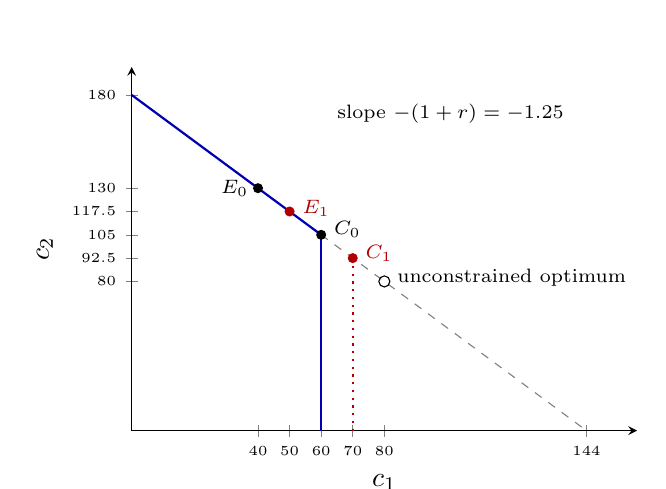
\begin{tikzpicture}
\begin{axis}[width=8cm,height=6.2cm,axis lines=left,xmin=0,xmax=160,ymin=0,ymax=195,
  xlabel={$c_1$},ylabel={$c_2$},xtick={40,50,60,70,80,144},ytick={80,92.5,105,117.5,130,180},
  every tick label/.append style={font=\tiny}]
\addplot[domain=60:144,dashed,gray]{1.25*(144-x)};
\addplot[domain=0:60,thick,blue!70!black]{1.25*(144-x)};
\draw[thick,blue!70!black](axis cs:60,105)--(axis cs:60,0);
\draw[dotted,thick,red!70!black](axis cs:70,92.5)--(axis cs:70,0);
\addplot[only marks,mark=*,mark size=1.6pt]coordinates{(40,130)(60,105)};
\addplot[only marks,mark=*,mark size=1.6pt,red!70!black]coordinates{(50,117.5)(70,92.5)};
\addplot[only marks,mark=o,mark size=2pt]coordinates{(80,80)};
\node[font=\scriptsize,anchor=east] at (axis cs:40,130){$E_0$};
\node[font=\scriptsize,anchor=west,red!70!black] at (axis cs:51,119){$E_1$};
\node[font=\scriptsize,anchor=west] at (axis cs:61,108){$C_0$};
\node[font=\scriptsize,anchor=west,red!70!black] at (axis cs:71,95){$C_1$};
\node[font=\scriptsize,anchor=west] at (axis cs:81,82){unconstrained optimum};
\node[font=\scriptsize,anchor=west] at (axis cs:62,170){slope $-(1+r)=-1.25$};
\end{axis}
\end{tikzpicture}\\
{\footnotesize Figure 2. The budget line is the same before and after the swap ($W=144$); the endowment slides
from $E_0$ to $E_1$ along it. The limit $c_1\le y_1-\tau_1+b$ moves from 60 to 70, so the constrained choice moves
from $C_0$ to $C_1$.}
\end{center}
\intuition{Ricardian equivalence needs the household to be able to move resources across periods at $r$.
When the limit binds, the tax cut is the loan the market would not give, and it is consumed one-for-one.}
\refbib{Kurlat \S6.2--\S6.4, pp.~120--126.}
\rubric{
\item (i) PV argument and $\Delta c_1=\Delta c_2=0$, $\Delta a=\Delta$: 2 pts.
\item (ii) Binding check and $c_1$ before/after: 1.5 pts (diagram with kink, labelled axes and points counts here).
\item (iii) Two examples: 1.5 pts (0.75 each).
\item Proving PV-only and then stating ``timing matters'' in the unconstrained case: max.\ 2 pts. One example only: $-0.75$.
}
\end{sol}
\begin{sol}
\gap{Lista 3, 1(a)(d) (never solved for $a$); 1(c) (right sign condition, opposite words); 1(e) (PV proved, then ``timing matters''); 2(b) (one example where two were asked).}
\end{sol}

% =============================================================================
\block{IV}{Money, inflation and AD--AS}{Lectures 7--9; Kurlat chs.~10--11; Benigno (2015) \,\textbullet\, 25 points}

\question{(10 points) Objective items.}

\textbf{a)} (3 points) About the quantity equation $MV=PY$:
\begin{options}
\item It is a theory of money demand: with $Y$ fixed, doubling $M$ doubles $P$ at every horizon.
\item It is an identity which proves neutrality, because $V$ and $Y$ are constant by definition.
\item It is a behavioural equation: $V$ is a structural parameter that the central bank sets.
\item It is an identity, since $V\equiv PY/M$; causation needs assumptions on $V$ and on what is exogenous.
\item It is an identity which proves causation runs from $P$ to $M$, because firms set prices first.
\end{options}
\answer{D}
\begin{sol}
\step{residual}{$V$ is measured as $PY/M$, so the equation holds for any data. It becomes a theory only with
an assumption on $V$ (e.g.\ stable, or given by a money-demand model) and on which variable is exogenous.}
\refbib{Kurlat \S10.4, pp.~199--204; \S11.2.}
\gap{Lista 6, 1(a): $V$ as a residual; causation needs an assumption.}
\end{sol}

\medskip
\textbf{b)} (3 points) In steady state with constant $i$, $\pi=\mu-\eta g$. The central bank targets $\pi^*=3\%$
with $g=2\%$ and sets $\mu$ assuming $\eta=1$ (Cambridge). Money demand is actually Baumol--Tobin. Inflation is:
\begin{options}
\item $2\%$
\item $3\%$
\item $4\%$
\item $5\%$
\item $6\%$
\end{options}
\answer{C}
\begin{sol}
\step{compute}{Chosen $\mu=\pi^*+1\cdot g=5\%$. Baumol--Tobin: $\eta=\tfrac12$, so $\pi=5\%-\tfrac12\cdot2\%=\res{4\%}$.
Desired real balances grow at $1\%$, not $2\%$: the extra money goes into prices.}
\refbib{Kurlat \S11.2, pp.~205--215.}
\gap{Lista 6, 2(b): inflation-targeting error formula.}
\end{sol}

\medskip
\textbf{c)} (2 points, T or F) When the central bank targets the nominal interest rate, the money-market
equilibrium $M=p\,m^D(Y,i)$ determines the quantity of money.
\answer{True}
\begin{sol}
\step{endogenous $M$}{With $i$ fixed by policy, and $p$, $Y$ given, $M$ must supply whatever $p\,m^D(Y,i)$ demands: the
central bank accommodates by open-market operations. Under a money target it is the reverse: $M$ given, $i$ adjusts.}
\refbib{Kurlat \S11.1--\S11.2; Benigno \S3 (policy sets $i$).}
\gap{Lista 6, 1(d): under an interest-rate target the money market determines $M$.}
\end{sol}

\medskip
\textbf{d)} (2 points, T or F) In Benigno's AD--AS model, a temporary rise in firms' desired mark-up
shifts the AD curve to the left.
\answer{False}
\begin{sol}
\step{which curve}{The mark-up enters the price-setting (AS) block: natural output falls, AS shifts up/left. AD comes
from the Euler equation and the policy rule, where $\mu$ does not appear: AD does not move (stagflation along AD).}
\refbib{Benigno (2015) \S4 and \S7.}
\gap{Shift of vs movement along AD/AS (taxonomy).}
\end{sol}

% -----------------------------------------------------------------------------
\question{(15 points) Pix and the demand for money. Since 2020 Pix, Brazil's instant-payment
system, has lowered the cost of turning deposits into means of payment. Model real money demand with
Baumol--Tobin, $m^D=\sqrt{\dfrac{FY}{2i}}$, where $F$ is the real cost of each conversion. Assume real
output grows at $g=2\%$, $F$ falls at the constant rate $\dot F/F=f=-4\%$, and $i$ is constant. The
money market clears: $M=p\,m^D(Y,i,F)$.}

\textbf{a)} (5 points) Derive velocity $V$ implied by this model. Explain why $V$ is not constant, and
compute its growth rate under the assumptions above. Interpret velocity in words.
\answerspace
\begin{sol}
\step{definition}{$V\equiv\dfrac{pY}{M}=\dfrac{pY}{p\,m^D}=\dfrac{Y}{\sqrt{FY/2i}}=\res{\sqrt{\dfrac{2iY}{F}}}$.}
\step{not constant}{$V$ depends on $i$ (opportunity cost of holding money $\uparrow\Rightarrow V\uparrow$), on $Y$
(economies of scale in cash management, $\partial\ln V/\partial\ln Y=\tfrac12$) and on $F$ (payment technology,
$\partial\ln V/\partial\ln F=-\tfrac12$).}
\step{growth}{$\dfrac{\dot V}{V}=\tfrac12\dfrac{\dot i}{i}+\tfrac12 g-\tfrac12 f=0+1\%+2\%=\res{3\%\ \text{per year}}$.}
\step{interpret}{$V$ is the number of times the average real balance is spent per period. In $MV=PY$ it
is a residual; Baumol--Tobin gives it a theory: cheaper conversions $\to$ smaller average balances per real
transaction $\to$ each real balance turns over faster.}
\refbib{Kurlat \S10.4, pp.~199--204.}
\rubric{
\item $V=\sqrt{2iY/F}$ derived: 2 pts.
\item Dependence on $i$, $Y$, $F$ with signs: 1 pt. Growth $3\%$: 1 pt. Interpretation: 1 pt.
\item Treating $V$ as constant or exogenous: max.\ 2 pts.
}
\end{sol}

\textbf{b)} (5 points) By totally differentiating $M=p\,m^D(Y,i,F)$ with respect to time, show that in
steady state $\pi=\mu-\tfrac12(g+f)$. Before Pix ($f=0$) the BCB grew money at the rate that delivered
$\pi=3\%$. Which money growth $\mu$ delivers $3\%$ after Pix? What inflation results if the BCB keeps the
old $\mu$? Explain the mechanism in words.
\answerspace
\begin{sol}
\step{differentiate}{$\dot M=\dot p\,m^D+p\left[\dfrac{\partial m^D}{\partial Y}\dot Y+\underbrace{\dfrac{\partial m^D}{\partial i}\dot i}_{=0\ (i\ \text{const.})}+\dfrac{\partial m^D}{\partial F}\dot F\right]$.}
\step{divide by $M=p\,m^D$}{$\mu=\pi+\underbrace{\dfrac{\partial m^D}{\partial Y}\dfrac{Y}{m^D}}_{\eta_Y}g+\underbrace{\dfrac{\partial m^D}{\partial F}\dfrac{F}{m^D}}_{\eta_F}f$.
From $m^D=(FY/2i)^{1/2}$: $\eta_Y=\eta_F=\tfrac12$ $\Rightarrow$ $\res{\pi=\mu-\tfrac12(g+f)}$.}
\step{before Pix}{$f=0$: $\mu=\pi^*+\tfrac12g=3\%+1\%=4\%$.}
\step{after Pix}{$\mu=\pi^*+\tfrac12(g+f)=3\%+\tfrac12(2\%-4\%)=3\%-1\%=\res{2\%}$.
Keeping $\mu=4\%$: $\pi=4\%-\tfrac12(-2\%)=\res{5\%}$.}
\step{mechanism}{$F\downarrow\to$ households hold smaller real balances $\to$ desired real money grows at
$\tfrac12(g+f)=-1\%$ instead of $+1\%$ $\to$ the same $\mu=4\%$ chases a \emph{shrinking} demand for real balances
$\to$ excess money $\to p$ grows faster: $\pi=5\%$. Equivalently, velocity rises at $3\%$. It is lower money
\emph{demand}, not ``cheap money''.}
\refbib{Kurlat \S11.2, pp.~205--215.}
\rubric{
\item Total differentiation with $\dot i=0$ struck: 1 pt. Elasticities named and $=\tfrac12$: 1 pt.
\item $\mu=2\%$ and $\pi=5\%$: 2 pts (1 each). Mechanism via money demand/velocity: 1 pt.
\item Explaining the effect as ``cheaper money'' or ``more money supply'': max.\ 3 pts. Arithmetic slip: $-1$.
}
\end{sol}

\textbf{c)} (5 points) Suppose instead the BCB sets the Selic (an interest-rate target $i^*$) and lets the
money supply be whatever it must be. When Pix lowers $F$, what adjusts in the money market in the short
run (prices sticky)? Is the Pix effect inflationary under this regime in the long run? Contrast with the
money-growth rule of (b).
\answerspace
\begin{sol}
\step{short run}{$F\downarrow\Rightarrow m^D\downarrow$ at every $i$ (curve shifts left). If $M$ stayed put, excess money
would push $i$ below $i^*$. To hold $i=i^*$ the BCB drains money (sells bonds):
$F\downarrow\to m^D\downarrow\to$ BCB sells bonds $\to M\downarrow$, $i=i^*$ unchanged $\to$ AD unchanged $\to y,p$ unchanged.
\res{\text{$M$ adjusts; $i$ does not.}}}
\step{long run}{$\pi$ is pinned by the target: $\pi=3\%$. Money growth becomes endogenous:
$\mu=\pi+\tfrac12(g+f)=3\%+\tfrac12(2\%-4\%)=\res{2\%}$. \res{\text{Not inflationary}}; Pix shows up only as slower
growth of money aggregates and rising velocity.}
\step{contrast}{Under a money-growth rule ($\mu=4\%$ fixed) the same shock raises $\pi$ to $5\%$, as in (b). The regime
decides whether a money-demand shock reaches prices: with an $i$ target the central bank absorbs it.}
\begin{center}
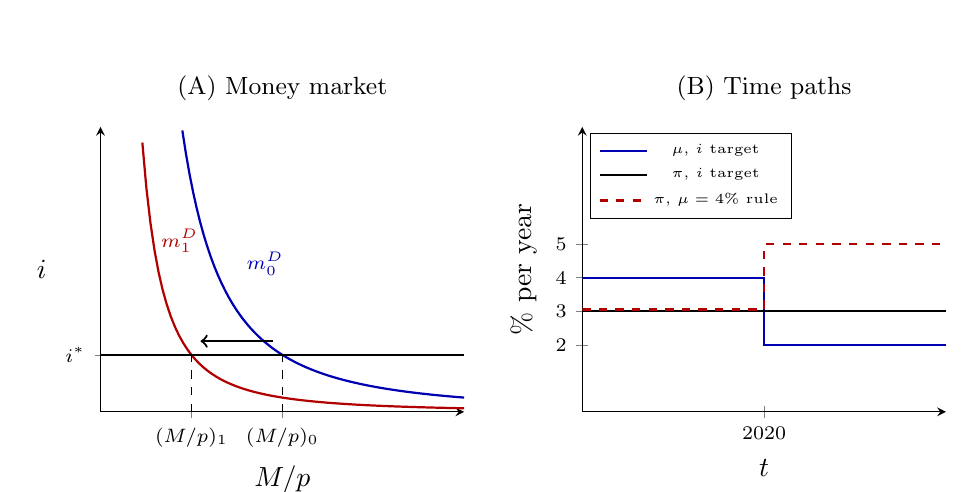
\begin{tikzpicture}
\begin{axis}[name=mm,width=6.2cm,height=5.2cm,axis lines=left,xmin=0,xmax=4,ymin=0,ymax=2.5,
  xlabel={$M/p$},ylabel={$i$},xtick={1,2},xticklabels={$(M/p)_1$,$(M/p)_0$},ylabel style={rotate=-90},ytick={0.5},yticklabels={$i^*$},
  title={\small (A) Money market},every tick label/.append style={font=\scriptsize}]
\addplot[domain=0.9:4,samples=80,thick,blue!70!black]{2/x^2};
\node[font=\scriptsize,blue!70!black,anchor=west] at (axis cs:1.5,1.3){$m^D_0$};
\addplot[domain=0.46:4,samples=80,thick,red!70!black]{0.5/x^2};
\node[font=\scriptsize,red!70!black] at (axis cs:0.87,1.5){$m^D_1$};
\addplot[thick,black]coordinates{(0,0.5)(4,0.5)};
\draw[dashed](axis cs:2,0)--(axis cs:2,0.5);
\draw[dashed](axis cs:1,0)--(axis cs:1,0.5);
\draw[->,thick](axis cs:1.9,0.62)--(axis cs:1.1,0.62);
\end{axis}
\begin{axis}[at={(mm.east)},anchor=west,xshift=1.5cm,width=6.2cm,height=5.2cm,axis lines=left,
  xmin=-5,xmax=5,ymin=0,ymax=8.5,xlabel={$t$},ylabel={\% per year},xtick={0},xticklabels={2020},
  ytick={2,3,4,5},title={\small (B) Time paths},every tick label/.append style={font=\scriptsize},
  legend style={font=\tiny,at={(0.02,0.98)},anchor=north west}]
\addplot[thick,blue!70!black]coordinates{(-5,4)(0,4)(0,2)(5,2)};
\addlegendentry{$\mu$, $i$ target}
\addplot[thick,black]coordinates{(-5,3)(5,3)};
\addlegendentry{$\pi$, $i$ target}
\addplot[dashed,thick,red!70!black]coordinates{(-5,3.05)(0,3.05)(0,5)(5,5)};
\addlegendentry{$\pi$, $\mu=4\%$ rule}
\end{axis}
\end{tikzpicture}\\
{\footnotesize Figure 3. (A) Lower $F$ shifts money demand left from $m^D_0=m^D(F_0)$ to $m^D_1=m^D(F_1)$ (drawn for $F_1=F_0/4$, which halves $m^D$); at $i^*$ real balances fall from $(M/p)_0$ to $(M/p)_1$.
(B) Under the $i$ target $\mu$ falls from 4\% to 2\% and $\pi$ stays at 3\%; under a fixed $\mu=4\%$, $\pi$ rises to 5\%.}
\end{center}
\intuition{Money is endogenous under an interest-rate rule: the central bank supplies the money people want at $i^*$.
A payment innovation that lowers money demand therefore changes $M$, not $i$, and leaves AD and inflation alone.}
\refbib{Kurlat \S11.1--\S11.2, pp.~205--215; Benigno (2015) \S3 (the central bank sets $i$).}
\rubric{
\item Short run: $m^D$ shifts left, $M$ adjusts, $i$ unchanged, no AD effect: 2 pts (arrow chain or diagram with labelled axes, curves and shift direction).
\item Long run: $\pi$ anchored, $\mu$ endogenous $=2\%$: 2 pts. Contrast with the money rule: 1 pt.
\item Stating that the BCB keeps $M$ fixed (or that $i$ falls) under an $i$ target: max.\ 2 pts.
}
\end{sol}
\begin{sol}
\gap{Lista 6, 1(a)(b) ($V$ a residual, velocity interpreted); 1(c) (mechanism; flexible-price neutrality: in the long run only $\pi$ and nominal aggregates move); 1(d) ($M$ endogenous under an $i$ target); 2(c) (falling $F$ = lower money demand, not ``cheap money'').}
\end{sol}

\end{document}
